\documentclass[a4paper,12pt,openright,notitlepage,twoside]{book}
\raggedbottom % lascia alla fine delle pagine lo spazio invece che adattarle


% pacchetti da caricare
\usepackage[T1]{fontenc} % definisce i caratteri di output
\usepackage[utf8]{inputenc} % definisce i caratteri di input
\usepackage[english]{babel} % definisce la lingua del documento
\usepackage[headheight=15pt]{geometry} % definisce i margini del documento
\geometry{a4paper,top=30mm,bottom=30mm,left=30mm,right=25mm,heightrounded,bindingoffset=3mm}
\usepackage{fancyhdr} % serve per gestire intestazione e piè di pagina
\pagestyle{fancy}
\usepackage{emptypage} % serve per fare le pagine vuote
\usepackage[pdftex]{hyperref} % serve per ottenere links e indice cliccabili
\hypersetup{colorlinks=true,allcolors=black}
\usepackage{microtype} % migliora la scrittura del testo
\usepackage{appendix} % serve per personalizzare l'appendice
\usepackage[printonlyused]{acronym} % serve per creare l'elenco degli acronimi
\usepackage{eurosym} % serve per scrivere il singolo dell'euro
\usepackage{siunitx} % serve per mettere le unita` di misura nel SI
\usepackage{mathtools} % serve per fare le formule matematiche (carica anche AMSMATH)
\usepackage{booktabs} % serve per fare le tabelle più belle
\usepackage{multirow} % serve per fare le tabelle con righe complesse
\usepackage{pgfplotstable} % serve per fare tabelle da file con dati tabulati
\usepackage{graphicx} % serve per fare le figure
\usepackage{tikz} % serve per fare i grafici
\usetikzlibrary{shapes}
\usepackage{pgfplots} % serve a fare i grafici anche lui
\pgfplotsset{compat=1.14}
\usepackage{subcaption} % serve per aggiungere la didascalia alle figure composte (carica anche CAPTION)
\captionsetup{font=small,labelsep=period,format=hang,tableposition=top,figureposition=bottom}
\usepackage{tocloft} % serve per fare le liste di figure e tabelle più belle
\usepackage{cite} % serve per mettere le citazioni bibliografiche
\usepackage{amsmath,amsfonts,amsthm,bm} % Math packages

\usepackage[ruled,vlined,linesnumbered]{algorithm2e}

\usepackage{soul}
\usepackage{color}

\usepackage{listings}


\definecolor{dkgreen}{rgb}{0,0.6,0}
\definecolor{gray}{rgb}{0.5,0.5,0.5}
\definecolor{mauve}{rgb}{0.58,0,0.82}
\definecolor{gray}{rgb}{0.4,0.4,0.4}
\definecolor{darkblue}{rgb}{0.0,0.0,0.6}
\definecolor{lightblue}{rgb}{0.0,0.0,0.9}
\definecolor{cyan}{rgb}{0.0,0.6,0.6}
\definecolor{darkred}{rgb}{0.6,0.0,0.0}

\definecolor{purple}{HTML}{710193}
\definecolor{green}{HTML}{028A0F}

\lstset{
	basicstyle=\ttfamily,
	columns=fullflexible,
	showstringspaces=false,
	numbers=left,                   % where to put the line-numbers
	numberstyle=\tiny\color{gray},  % the style that is used for the line-numbers
	stepnumber=1,
	numbersep=5pt,                  % how far the line-numbers are from the code
	backgroundcolor=\color{white},      % choose the background color. You must add \usepackage{color}
	showspaces=false,               % show spaces adding particular underscores
	showstringspaces=false,         % underline spaces within strings
	showtabs=false,                 % show tabs within strings adding particular underscores
	frame=none,                   % adds a frame around the code
	rulecolor=\color{black},        % if not set, the frame-color may be changed on line-breaks within not-black text (e.g. commens (green here))
	tabsize=2,                      % sets default tabsize to 2 spaces
	captionpos=b,                   % sets the caption-position to bottom
	breaklines=true,                % sets automatic line breaking
	breakatwhitespace=false,        % sets if automatic breaks should only happen at whitespace
	title=\lstname,                   % show the filename of files included with \lstinputlisting;
	% also try caption instead of title  
	commentstyle=\color{gray}\upshape
}

\lstdefinelanguage{XML}
{
  morestring=[s][\color{darkblue}]{"}{"},
  morestring=[s][\color{black}]{>}{<},
  morecomment=[s]{<?}{?>},
  morecomment=[s][\color{dkgreen}]{<!--}{-->},
  stringstyle=\color{black},
  identifierstyle=\color{green},
  keywordstyle=\color{purple},
  morekeywords={xmlns,version,type, dimensions, from, to, first, second, value, data:vector, use-data, write-data, read-data, use-mesh, limit}% list your attributes here
}

\lstdefinelanguage{mbdyn}
{
  morestring=[s][\color{darkblue}]{"}{"},
  morecomment=[l]{\#},
  morecomment=[s]{/*}{*/},
  morecomment=[n]{(*}{*)},
  stringstyle=\color{black},
  identifierstyle=\color{red},
  keywordstyle=\color{blue},
  morekeywords={begin, end, control data, initial value ,problem}% list your attributes here
}

\colorlet{punct}{red!60!black}
\definecolor{background}{HTML}{EEEEEE}
\definecolor{delim}{RGB}{20,105,176}
\colorlet{numb}{magenta!60!black}

\lstdefinelanguage{json}{
	basicstyle=\normalfont\ttfamily,
	numbers=left,
	numberstyle=\scriptsize,
	stepnumber=1,
	numbersep=8pt,
	showstringspaces=false,
	breaklines=true,
	frame=lines,
%	backgroundcolor=\color{background},
	literate=
	*{0}{{{\color{numb}0}}}{1}
	{1}{{{\color{numb}1}}}{1}
	{2}{{{\color{numb}2}}}{1}
	{3}{{{\color{numb}3}}}{1}
	{4}{{{\color{numb}4}}}{1}
	{5}{{{\color{numb}5}}}{1}
	{6}{{{\color{numb}6}}}{1}
	{7}{{{\color{numb}7}}}{1}
	{8}{{{\color{numb}8}}}{1}
	{9}{{{\color{numb}9}}}{1}
	{:}{{{\color{punct}{:}}}}{1}
	{,}{{{\color{punct}{,}}}}{1}
	{\{}{{{\color{delim}{\{}}}}{1}
	{\}}{{{\color{delim}{\}}}}}{1}
	{[}{{{\color{delim}{[}}}}{1}
	{]}{{{\color{delim}{]}}}}{1},
}



\usepackage{hyperref}
\hypersetup{
	colorlinks=true,
	linkcolor=red,
	filecolor=magenta,      
	urlcolor=blue,
}

\urlstyle{same}

% modifiche dei comandi
\renewcommand{\chaptermark}[1]{\markboth{\chaptername\ \thechapter.\ #1}{}} % modifica l'intestazione con il nome/numero del capitolo
\renewcommand{\sectionmark}[1]{\markright{\thesection.\ #1}} % modifica l'intestazione con il nome/numero dela sezione
\renewcommand{\cftfigfont}{Figure } % per aggiungere "Figure " nella lista delle figure
\renewcommand{\cfttabfont}{Table } % per aggiungere "Table " nella lista delle tabelle


\DeclareMathOperator*{\argmin}{argmin} % thin space, limits underneath in displays


% Keywords command
\providecommand{\keywords}[1]
{
  \small	
  \textit{\textbf{Keywords---}} #1
}


% dichiarazioni personalizzate
\DeclarePairedDelimiter{\abs}{\lvert}{\rvert} % per fare il valore assoluto
\DeclarePairedDelimiter{\norma}{\lVert}{\rVert} % per fare la norma



\begin{document}

\frontmatter % serve per mettere i numeri romani come numeri di pagina 
\thispagestyle{empty} % serve per rimuovere tutte le impostazioni delle pagine dalla prima pagina

% FRONTESPIZIO
\begin{center}
% Intestazione
\Large{\textbf{Politecnico di Milano}} \\
\vspace{-4mm}
\rule{\textwidth}{0.4pt}
\normalsize{SCHOOL OF INDUSTRIAL AND INFORMATION ENGINEERING} \\
\normalsize{Master of Science -- Aerospace Engineering} \\
\vspace{20mm}
% Logo Politecnico
\begin{figure}[h!]
\centering
\includegraphics[height=0.15\textheight]{images/logo-polimi}
\end{figure}
\vspace{22mm}
% Titolo Tesi
\huge{\textbf{Thesis Title}} \\
\vspace{32mm}
\end{center}

% Relatore/Correlatore
\begin{flushleft}
\normalsize{Supervisor} \\
\small{\textbf{Title Name SURMANE}} \\
\vspace{5mm}
\normalsize{Co-Supervisor} \\
\small{\textbf{Title Name SURNAME}} \\
\end{flushleft}
\vspace{20mm}

% Autore
\begin{flushright}
\normalsize{Candidate} \\
\small{\textbf{Claudio CACCIA -- 820091}} \\
\end{flushright}
\vspace{15mm}

% Piè Di Pagina
\begin{center}
\rule{\textwidth}{0.4pt}
\small{\textbf{Academic Year 2019 -- 2020}}
\end{center}


% modifica intestazione e piè di pagina del corpo del documento
\fancyhead{} % cancella tutti i campi dell'intestazione
\fancyfoot{} % cancella tutti i campi del piè di pagina
\fancyhead[LE,RO]{\leftmark}
\fancyfoot[LE,RO]{\thepage}
\renewcommand{\headrulewidth}{0.4pt}
\renewcommand{\footrulewidth}{0pt}


% carico le varie parti della tesi
\chapter*{Acknowledgements}
\label{cha:acknowledgements}
\markboth{Acknowledgements}{}
\addcontentsline{toc}{chapter}{Acknowledgements}

First, I would like to thank my supervisors, prof. Pierangelo Masarati and prof. Marco Morandini for giving me the opportunity to work on this fascinating topic and  letting me do it at my own pace. I had the chance to attend  to their courses and  that inspired me to improve my knowledge.

I would also thank them for their support and suggestions, even if these difficult times made everything a little more complicated. 

My special thanks go to the preCICE community, to Benjamin Uekermann, Gerasimos ``Makis'' Chourdakis and many others who were happy to exchange ideas and shared their knowledge and experience, helping me better understand the most difficult aspects of this subject.

Finally, but not least importantly, I owe my gratitude to Eleonora Colombo, who let me endlessly talk about my doubts and difficulties. She helped me put everything in perspective and gave me the motivation to pursue my goal, independently from everything else. Without her support this would not have been possible. 

%First and foremost, I would like to deeply thank my supervisor, Benjamin Uekermann, for
%his support. His vivid interest on the topic and his very helpful advices made my thesis a
%very pleasant learning experience.


%Additionally, I would like to thank Lucía Cheung Yau, whose excellent work I had the
%challenging mission to continue. Her aid in the beginning of my Thesis was invaluable. I
%also want to thank Babak Gholami for kindly providing us with the results of Lucía’s thesis,
%which was written in cooperation with SimScale GmbH.
%The tools I used in my thesis, mainly preCICE and OpenFOAM, are developed as
%free/open source software. They are also based on other free software projects, including
%the Doxygen documentation generator. Projects like these make me feel very glad of
%the free software community and I hope that my contribution will also be useful.
%The TUM English Writing Center helped me improve my understanding of the English
%language and the clarity of my prose. I am very thankful for the time they devoted to me
%during the Thesis Writers’ Workshop, as well as to our individual appointments.
%My Master’s studies were financially aided by a scholarship from the German Academic
%Exchange Service (DAAD) and I am very grateful of their support.
%Finally, I owe my deepest gratitude to my friends and family, whose endless support was
%crucial for my studies. Special thanks go to my parents and to my friend Myrto, who were
%there when their support was needed the most.
% !TeX spellcheck = en_US
\chapter*{Abstract}
\label{cha:abstract}
\markboth{Abstract}{}
\addcontentsline{toc}{chapter}{Abstract}


The computer simulation of \acrfull{fsi} phenomena allows to gain more insight on complex interactions and behaviors of solids immersed in fluid flows, helping predict their effects. Applications range from aeroelasticity, to turbomachinery, or biomechanics, just to name a few. 

It is possible to perform those simulations in different ways: one of them involves a technique known as \textit{partitioned algorithm}. A partitioned algorithm aims at solving a \acrshort{fsi} problem basically by means of three elements, which include a fluid solver, a structural solver and a third component which performs the interaction between the other two. The advantage of this technique consists in reusing and adapting already developed and optimized solvers and connect them. 

In this thesis, the \acrfull{mbdyn} has been linked to the multiphysics coupling library \acrfull{precice}, with the purpose of extending \acrshort{mbdyn} capabilities in the field of \acrshort{fsi} simulations.

For this reason, an \textit{adapter}(i.e. a piece of connecting code, in this case written in C++), has been developed to implement this coupling.

Coupling \acrshort{mbdyn} with \acrshort{precice} represents and advantage and an extension of capabilities, because many other adapters for the fluid side have already been developed for this library. It is then  possible and simple to choose among a considerable number of fluid solvers, including many well-validated open source and commercial codes. On the other hand, with a fully integrated \textit{MBDyn adapter}, the library preCICE gains the opportunity to connect to a multibody dynamics software, which has not yet been completely developed.  

The coupling between \acrshort{mbdyn} and \acrshort{precice} has been successfully tested in different scenarios, including some well-known \acrshort{fsi} benchmark problems. Also some current limitations of applicability, emerged in one of those benchmarks, have been analyzed.

The current status of the adapter represents a good starting point to explore more in detail the behavior of the \acrshort{mbdyn}-\acrshort{precice} coupling even in more complex scenarios and to use it in real-world applications.


\vspace{5mm}


\keywords{fluid structure interaction, partitioned algorithms, multibody dynamics, MBDyn, preCICE}
\chapter*{Sommario}
\label{cha:sommario}
\markboth{Sommario}{}
\addcontentsline{toc}{chapter}{Sommario}

%TODO Tradurre abstract
% \chapter*{Extended Abstract}
\label{cha:extended_abstract}
\markboth{Extended Abstract}{}
\addcontentsline{toc}{chapter}{Extended Abstract}

Lorem ipsum dolor sit amet, consectetur adipisci elit, sed eiusmod tempor incidunt ut labore et dolore magna aliqua. Ut enim ad minim veniam, quis nostrum exercitationem ullam corporis suscipit laboriosam, nisi ut aliquid ex ea commodi consequatur. Quis aute iure reprehenderit in voluptate velit esse cillum dolore eu fugiat nulla pariatur. Excepteur sint obcaecat cupiditat non proident, sunt in culpa qui officia deserunt mollit anim id est laborum. Lorem ipsum dolor sit amet, consectetur adipisci elit, sed eiusmod tempor incidunt ut labore et dolore magna aliqua. Ut enim ad minim veniam, quis nostrum exercitationem ullam corporis suscipit laboriosam, nisi ut aliquid ex ea commodi consequatur. Quis aute iure reprehenderit in voluptate velit esse cillum dolore eu fugiat nulla pariatur. Excepteur sint obcaecat cupiditat non proident, sunt in culpa qui officia deserunt mollit anim id est laborum. Lorem ipsum dolor sit amet, consectetur adipisci elit, sed eiusmod tempor incidunt ut labore et dolore magna aliqua. Ut enim ad minim veniam, quis nostrum exercitationem ullam corporis suscipit laboriosam, nisi ut aliquid ex ea commodi consequatur. Quis aute iure reprehenderit in voluptate velit esse cillum dolore eu fugiat nulla pariatur. Excepteur sint obcaecat cupiditat non proident, sunt in culpa qui officia deserunt mollit anim id est laborum. Lorem ipsum dolor sit amet, consectetur adipisci elit, sed eiusmod tempor incidunt ut labore et dolore magna aliqua. Ut enim ad minim veniam, quis nostrum exercitationem ullam corporis suscipit laboriosam, nisi ut aliquid ex ea commodi consequatur. Quis aute iure reprehenderit in voluptate velit esse cillum dolore eu fugiat nulla pariatur. Excepteur sint obcaecat cupiditat non proident, sunt in culpa qui officia deserunt mollit anim id est laborum. Lorem ipsum dolor sit amet, consectetur adipisci elit, sed eiusmod tempor incidunt ut labore et dolore magna aliqua. Ut enim ad minim veniam, quis nostrum exercitationem ullam corporis suscipit laboriosam, nisi ut aliquid ex ea commodi consequatur. Quis aute iure reprehenderit in voluptate velit esse cillum dolore eu fugiat nulla pariatur. Excepteur sint obcaecat cupiditat non proident, sunt in culpa qui officia deserunt mollit anim id est laborum. Lorem ipsum dolor sit amet, consectetur adipisci elit, sed eiusmod tempor incidunt ut labore et dolore magna aliqua. Ut enim ad minim veniam, quis nostrum exercitationem ullam corporis suscipit laboriosam, nisi ut aliquid ex ea commodi consequatur. Quis aute iure reprehenderit in voluptate velit esse cillum dolore eu fugiat nulla pariatur. Excepteur sint obcaecat cupiditat non proident, sunt in culpa qui officia deserunt mollit anim id est laborum. Lorem ipsum dolor sit amet, consectetur adipisci elit, sed eiusmod tempor incidunt ut labore et dolore magna aliqua. Ut enim ad minim veniam, quis nostrum exercitationem ullam corporis suscipit laboriosam, nisi ut aliquid ex ea commodi consequatur. Quis aute iure reprehenderit in voluptate velit esse cillum dolore eu fugiat nulla pariatur. Excepteur sint obcaecat cupiditat non proident, sunt in culpa qui officia deserunt mollit anim id est laborum. Lorem ipsum dolor sit amet, consectetur adipisci elit, sed eiusmod tempor incidunt ut labore et dolore magna aliqua. Ut enim ad minim veniam, quis nostrum exercitationem ullam corporis suscipit laboriosam, nisi ut aliquid ex ea commodi consequatur. Quis aute iure reprehenderit in voluptate velit esse cillum dolore eu fugiat nulla pariatur. Excepteur sint obcaecat cupiditat non proident, sunt in culpa qui officia deserunt mollit anim id est laborum. Lorem ipsum dolor sit amet, consectetur adipisci elit, sed eiusmod tempor incidunt ut labore et dolore magna aliqua. Ut enim ad minim veniam, quis nostrum exercitationem ullam corporis suscipit laboriosam, nisi ut aliquid ex ea commodi consequatur. Quis aute iure reprehenderit in voluptate velit esse cillum dolore eu fugiat nulla pariatur. Excepteur sint obcaecat cupiditat non proident, sunt in culpa qui officia deserunt mollit anim id est laborum. Lorem ipsum dolor sit amet, consectetur adipisci elit, sed eiusmod tempor incidunt ut labore et dolore magna aliqua. Ut enim ad minim veniam, quis nostrum exercitationem ullam corporis suscipit laboriosam, nisi ut aliquid ex ea commodi consequatur. Quis aute iure reprehenderit in voluptate velit esse cillum dolore eu fugiat nulla pariatur. Excepteur sint obcaecat cupiditat non proident, sunt in culpa qui officia deserunt mollit anim id est laborum. Lorem ipsum dolor sit amet, consectetur adipisci elit, sed eiusmod tempor incidunt ut labore et dolore magna aliqua. Ut enim ad minim veniam, quis nostrum exercitationem ullam corporis suscipit laboriosam, nisi ut aliquid ex ea commodi consequatur. Quis aute iure reprehenderit in voluptate velit esse cillum dolore eu fugiat nulla pariatur. Excepteur sint obcaecat cupiditat non proident, sunt in culpa qui officia deserunt mollit anim id est laborum. Lorem ipsum dolor sit amet, consectetur adipisci elit, sed eiusmod tempor incidunt ut labore et dolore magna aliqua. Ut enim ad minim veniam, quis nostrum exercitationem ullam corporis suscipit laboriosam, nisi ut aliquid ex ea commodi consequatur. Quis aute iure reprehenderit in voluptate velit esse cillum dolore eu fugiat nulla pariatur. Excepteur sint obcaecat cupiditat non proident, sunt in culpa qui officia deserunt mollit anim id est laborum. Lorem ipsum dolor sit amet, consectetur adipisci elit, sed eiusmod tempor incidunt ut labore et dolore magna aliqua. Ut enim ad minim veniam, quis nostrum exercitationem ullam corporis suscipit laboriosam, nisi ut aliquid ex ea commodi consequatur. Quis aute iure reprehenderit in voluptate velit esse cillum dolore eu fugiat nulla pariatur. Excepteur sint obcaecat cupiditat non proident, sunt in culpa qui officia deserunt mollit anim id est laborum. Lorem ipsum dolor sit amet, consectetur adipisci elit, sed eiusmod tempor incidunt ut labore et dolore magna aliqua. Ut enim ad minim veniam, quis nostrum exercitationem ullam corporis suscipit laboriosam, nisi ut aliquid ex ea commodi consequatur. Quis aute iure reprehenderit in voluptate velit esse cillum dolore eu fugiat nulla pariatur. Excepteur sint obcaecat cupiditat non proident, sunt in culpa qui officia deserunt mollit anim id est laborum. Lorem ipsum dolor sit amet, consectetur adipisci elit, sed eiusmod tempor incidunt ut labore et dolore magna aliqua. Ut enim ad minim veniam, quis nostrum exercitationem ullam corporis suscipit laboriosam, nisi ut aliquid ex ea commodi consequatur. Quis aute iure reprehenderit in voluptate velit esse cillum dolore eu fugiat nulla pariatur. Excepteur sint obcaecat cupiditat non proident, sunt in culpa qui officia deserunt mollit anim id est laborum. Lorem ipsum dolor sit amet, consectetur adipisci elit, sed eiusmod tempor incidunt ut labore et dolore magna aliqua. Ut enim ad minim veniam, quis nostrum exercitationem ullam corporis suscipit laboriosam, nisi ut aliquid ex ea commodi consequatur. Quis aute iure reprehenderit in voluptate velit esse cillum dolore eu fugiat nulla pariatur. Excepteur sint obcaecat cupiditat non proident, sunt in culpa qui officia deserunt mollit anim id est laborum. Lorem ipsum dolor sit amet, consectetur adipisci elit, sed eiusmod tempor incidunt ut labore et dolore magna aliqua. Ut enim ad minim veniam, quis nostrum exercitationem ullam corporis suscipit laboriosam, nisi ut aliquid ex ea commodi consequatur. Quis aute iure reprehenderit in voluptate velit esse cillum dolore eu fugiat nulla pariatur. Excepteur sint obcaecat cupiditat non proident, sunt in culpa qui officia deserunt mollit anim id est laborum. Lorem ipsum dolor sit amet, consectetur adipisci elit, sed eiusmod tempor incidunt ut labore et dolore magna aliqua. Ut enim ad minim veniam, quis nostrum exercitationem ullam corporis suscipit laboriosam, nisi ut aliquid ex ea commodi consequatur. Quis aute iure reprehenderit in voluptate velit esse cillum dolore eu fugiat nulla pariatur. Excepteur sint obcaecat cupiditat non proident, sunt in culpa qui officia deserunt mollit anim id est laborum. Lorem ipsum dolor sit amet, consectetur adipisci elit, sed eiusmod tempor incidunt ut labore et dolore magna aliqua. Ut enim ad minim veniam, quis nostrum exercitationem ullam corporis suscipit laboriosam, nisi ut aliquid ex ea commodi consequatur. Quis aute iure reprehenderit in voluptate velit esse cillum dolore eu fugiat nulla pariatur. Excepteur sint obcaecat cupiditat non proident, sunt in culpa qui officia deserunt mollit anim id est laborum. Lorem ipsum dolor sit amet, consectetur adipisci elit, sed eiusmod tempor incidunt ut labore et dolore magna aliqua. Ut enim ad minim veniam, quis nostrum exercitationem ullam corporis suscipit laboriosam, nisi ut aliquid ex ea commodi consequatur. Quis aute iure reprehenderit in voluptate velit esse cillum dolore eu fugiat nulla pariatur. Excepteur sint obcaecat cupiditat non proident, sunt in culpa qui officia deserunt mollit anim id est laborum. Lorem ipsum dolor sit amet, consectetur adipisci elit, sed eiusmod tempor incidunt ut labore et dolore magna aliqua. Ut enim ad minim veniam, quis nostrum exercitationem ullam corporis suscipit laboriosam, nisi ut aliquid ex ea commodi consequatur. Quis aute iure reprehenderit in voluptate velit esse cillum dolore eu fugiat nulla pariatur. Excepteur sint obcaecat cupiditat non proident, sunt in culpa qui officia deserunt mollit anim id est laborum. Lorem ipsum dolor sit amet, consectetur adipisci elit, sed eiusmod tempor incidunt ut labore et dolore magna aliqua. Ut enim ad minim veniam, quis nostrum exercitationem ullam corporis suscipit laboriosam, nisi ut aliquid ex ea commodi consequatur. Quis aute iure reprehenderit in voluptate velit esse cillum dolore eu fugiat nulla pariatur. Excepteur sint obcaecat cupiditat non proident, sunt in culpa qui officia deserunt mollit anim id est laborum. Lorem ipsum dolor sit amet, consectetur adipisci elit, sed eiusmod tempor incidunt ut labore et dolore magna aliqua. Ut enim ad minim veniam, quis nostrum exercitationem ullam corporis suscipit laboriosam, nisi ut aliquid ex ea commodi consequatur. Quis aute iure reprehenderit in voluptate velit esse cillum dolore eu fugiat nulla pariatur. Excepteur sint obcaecat cupiditat non proident, sunt in culpa qui officia deserunt mollit anim id est laborum. Lorem ipsum dolor sit amet, consectetur adipisci elit, sed eiusmod tempor incidunt ut labore et dolore magna aliqua. Ut enim ad minim veniam, quis nostrum exercitationem ullam corporis suscipit laboriosam, nisi ut aliquid ex ea commodi consequatur. Quis aute iure reprehenderit in voluptate velit esse cillum dolore eu fugiat nulla pariatur. Excepteur sint obcaecat cupiditat non proident, sunt in culpa qui officia deserunt mollit anim id est laborum. Lorem ipsum dolor sit amet, consectetur adipisci elit, sed eiusmod tempor incidunt ut labore et dolore magna aliqua. Ut enim ad minim veniam, quis nostrum exercitationem ullam corporis suscipit laboriosam, nisi ut aliquid ex ea commodi consequatur. Quis aute iure reprehenderit in voluptate velit esse cillum dolore eu fugiat nulla pariatur. Excepteur sint obcaecat cupiditat non proident, sunt in culpa qui officia deserunt mollit anim id est laborum. Lorem ipsum dolor sit amet, consectetur adipisci elit, sed eiusmod tempor incidunt ut labore et dolore magna aliqua. Ut enim ad minim veniam, quis nostrum exercitationem ullam corporis suscipit laboriosam, nisi ut aliquid ex ea commodi consequatur. Quis aute iure reprehenderit in voluptate velit esse cillum dolore eu fugiat nulla pariatur. Excepteur sint obcaecat cupiditat non proident, sunt in culpa qui officia deserunt mollit anim id est laborum. Lorem ipsum dolor sit amet, consectetur adipisci elit, sed eiusmod tempor incidunt ut labore et dolore magna aliqua. Ut enim ad minim veniam, quis nostrum exercitationem ullam corporis suscipit laboriosam, nisi ut aliquid ex ea commodi consequatur. Quis aute iure reprehenderit in voluptate velit esse cillum dolore eu fugiat nulla pariatur. Excepteur sint obcaecat cupiditat non proident, sunt in culpa qui officia deserunt mollit anim id est laborum. Lorem ipsum dolor sit amet, consectetur adipisci elit, sed eiusmod tempor incidunt ut labore et dolore magna aliqua. Ut enim ad minim veniam, quis nostrum exercitationem ullam corporis suscipit laboriosam, nisi ut aliquid ex ea commodi consequatur. Quis aute iure reprehenderit in voluptate velit esse cillum dolore eu fugiat nulla pariatur. Excepteur sint obcaecat cupiditat non proident, sunt in culpa qui officia deserunt mollit anim id est laborum. Lorem ipsum dolor sit amet, consectetur adipisci elit, sed eiusmod tempor incidunt ut labore et dolore magna aliqua. Ut enim ad minim veniam, quis nostrum exercitationem ullam corporis suscipit laboriosam, nisi ut aliquid ex ea commodi consequatur. Quis aute iure reprehenderit in voluptate velit esse cillum dolore eu fugiat nulla pariatur. Excepteur sint obcaecat cupiditat non proident, sunt in culpa qui officia deserunt mollit anim id est laborum. Lorem ipsum dolor sit amet, consectetur adipisci elit, sed eiusmod tempor incidunt ut labore et dolore magna aliqua. Ut enim ad minim veniam, quis nostrum exercitationem ullam corporis suscipit laboriosam, nisi ut aliquid ex ea commodi consequatur. Quis aute iure reprehenderit in voluptate velit esse cillum dolore eu fugiat nulla pariatur. Excepteur sint obcaecat cupiditat non proident, sunt in culpa qui officia deserunt mollit anim id est laborum. Lorem ipsum dolor sit amet, consectetur adipisci elit, sed eiusmod tempor incidunt ut labore et dolore magna aliqua. Ut enim ad minim veniam, quis nostrum exercitationem ullam corporis suscipit laboriosam, nisi ut aliquid ex ea commodi consequatur. Quis aute iure reprehenderit in voluptate velit esse cillum dolore eu fugiat nulla pariatur. Excepteur sint obcaecat cupiditat non proident, sunt in culpa qui officia deserunt mollit anim id est laborum. Lorem ipsum dolor sit amet, consectetur adipisci elit, sed eiusmod tempor incidunt ut labore et dolore magna aliqua. Ut enim ad minim veniam, quis nostrum exercitationem ullam corporis suscipit laboriosam, nisi ut aliquid ex ea commodi consequatur. Quis aute iure reprehenderit in voluptate velit esse cillum dolore eu fugiat nulla pariatur. Excepteur sint obcaecat cupiditat non proident, sunt in culpa qui officia deserunt mollit anim id est laborum. Lorem ipsum dolor sit amet, consectetur adipisci elit, sed eiusmod tempor incidunt ut labore et dolore magna aliqua. Ut enim ad minim veniam, quis nostrum exercitationem ullam corporis suscipit laboriosam, nisi ut aliquid ex ea commodi consequatur. Quis aute iure reprehenderit in voluptate velit esse cillum dolore eu fugiat nulla pariatur. Excepteur sint obcaecat cupiditat non proident, sunt in culpa qui officia deserunt mollit anim id est laborum. Lorem ipsum dolor sit amet, consectetur adipisci elit, sed eiusmod tempor incidunt ut labore et dolore magna aliqua. Ut enim ad minim veniam, quis nostrum exercitationem ullam corporis suscipit laboriosam, nisi ut aliquid ex ea commodi consequatur. Quis aute iure reprehenderit in voluptate velit esse cillum dolore eu fugiat nulla pariatur. Excepteur sint obcaecat cupiditat non proident, sunt in culpa qui officia deserunt mollit anim id est laborum. Lorem ipsum dolor sit amet, consectetur adipisci elit, sed eiusmod tempor incidunt ut labore et dolore magna aliqua. Ut enim ad minim veniam, quis nostrum exercitationem ullam corporis suscipit laboriosam, nisi ut aliquid ex ea commodi consequatur. Quis aute iure reprehenderit in voluptate velit esse cillum dolore eu fugiat nulla pariatur. Excepteur sint obcaecat cupiditat non proident, sunt in culpa qui officia deserunt mollit anim id est laborum. Lorem ipsum dolor sit amet, consectetur adipisci elit, sed eiusmod tempor incidunt ut labore et dolore magna aliqua. Ut enim ad minim veniam, quis nostrum exercitationem ullam corporis suscipit laboriosam, nisi ut aliquid ex ea commodi consequatur. Quis aute iure reprehenderit in voluptate velit esse cillum dolore eu fugiat nulla pariatur. Excepteur sint obcaecat cupiditat non proident, sunt in culpa qui officia deserunt mollit anim id est laborum. Lorem ipsum dolor sit amet, consectetur adipisci elit, sed eiusmod tempor incidunt ut labore et dolore magna aliqua. Ut enim ad minim veniam, quis nostrum exercitationem ullam corporis suscipit laboriosam, nisi ut aliquid ex ea commodi consequatur. Quis aute iure reprehenderit in voluptate velit esse cillum dolore eu fugiat nulla pariatur. Excepteur sint obcaecat cupiditat non proident, sunt in culpa qui officia deserunt mollit anim id est laborum. Lorem ipsum dolor sit amet, consectetur adipisci elit, sed eiusmod tempor incidunt ut labore et dolore magna aliqua. Ut enim ad minim veniam, quis nostrum exercitationem ullam corporis suscipit laboriosam, nisi ut aliquid ex ea commodi consequatur. Quis aute iure reprehenderit in voluptate velit esse cillum dolore eu fugiat nulla pariatur. Excepteur sint obcaecat cupiditat non proident, sunt in culpa qui officia deserunt mollit anim id est laborum. Lorem ipsum dolor sit amet, consectetur adipisci elit, sed eiusmod tempor incidunt ut labore et dolore magna aliqua. Ut enim ad minim veniam, quis nostrum exercitationem ullam corporis suscipit laboriosam, nisi ut aliquid ex ea commodi consequatur. Quis aute iure reprehenderit in voluptate velit esse cillum dolore eu fugiat nulla pariatur. Excepteur sint obcaecat cupiditat non proident, sunt in culpa qui officia deserunt mollit anim id est laborum. Lorem ipsum dolor sit amet, consectetur adipisci elit, sed eiusmod tempor incidunt ut labore et dolore magna aliqua. Ut enim ad minim veniam, quis nostrum exercitationem ullam corporis suscipit laboriosam, nisi ut aliquid ex ea commodi consequatur. Quis aute iure reprehenderit in voluptate velit esse cillum dolore eu fugiat nulla pariatur. Excepteur sint obcaecat cupiditat non proident, sunt in culpa qui officia deserunt mollit anim id est laborum.obcaecat cupiditat non proident, sunt in culpa qui officia deserunt mollit anim id est laborum. Lorem ipsum dolor sit amet, consectetur adipisci elit, sed eiusmod tempor incidunt ut labore et dolore magna aliqua. Ut enim ad minim veniam, quis nostrum exercitationem ullam corporis suscipit laboriosam, nisi ut aliquid ex ea commodi consequatur.
\cleardoublepage


% modifica intestazione indice
\fancyhead[LE,RO]{\nouppercase{\leftmark}} % cancella il tutto maiuscolo

% Indice 
\phantomsection
\tableofcontents
\addcontentsline{toc}{chapter}{\contentsname}
\cleardoublepage


% Lista delle Figure
\phantomsection
\listoffigures
\addcontentsline{toc}{chapter}{\listfigurename}
\cleardoublepage


% Lista delle Tabelle
\phantomsection
\listoftables
\addcontentsline{toc}{chapter}{\listtablename}
\cleardoublepage

% Lista del codice
\phantomsection
\lstlistoflistings
\addcontentsline{toc}{chapter}{\lstlistingname}
\cleardoublepage


\fancyhead[LE]{\leftmark}
\fancyhead[RO]{\rightmark}
\fancyfoot[LE,RO]{\thepage}

\mainmatter % serve per mettere i numeri arabi come numeri di pagina


% Capitoli Tesi
\chapter{Introduction}
\label{cha:intro}


% Interaction between a fluid and a solid happens everywhere


% TODO: initial claim, magari da limare

\acrfull{fsi} describes the mutual interaction between a moving or deformable object and a fluid in contact with it, surrounding or internal. It is present in various forms both in nature and in man-made systems: a leaf fluttering in the wind, water flowing underground or blood pumping in an artery are typical examples of fluid-structure interaction in nature. FSI occurs in engineered systems when modeling the behavior of turbomachinery, the flight characteristics of an aircraft, or the interaction of a building with the wind, just to name a few examples.

All the aforementioned problems go under the same  category of FSI, even if the nature of the interaction between the solid and fluid is different. Specifically, the intensity of the exchanged quantities and the effect in the fluid and solid domains vary among different problems.

%While many problems involve solid deformation as an integral part, there are many man-made problems in which the solid may be considered to move as a rigid body. It is also possible to have one-directional coupling between the fluid and solid in certain problems. For the sake of completeness and clarity, we classify the subject below.
There can be multiple ways to classify FSI problems, based on the flow physics and on the behavior of the body. Incompressible flow assumption is always made for liquid-solid interaction, while both compressible and incompressible flow assumptions are made when a gas interacts with a solid, depending on the flow properties and the kind of simulation. The main application of air-solid interaction considers the determination of aerodynamic forces on structures such as aircraft wings, which is often referred to as \textit{aeroelasticity}. Dynamic aeroelasticity is the topic that normally investigates the interaction between aerodynamic, elastic and inertial forces. Aerodynamic \textit{flutter} (i.e. the dynamic instability of an elastic structure in a fluid flow) is one of the severe consequences of aerodynamic forces. It is responsible for destructive effects in structures and a significant example of FSI problem.

The subject may also be classified considering the behavior of the structure interacting with the fluid: a solid can be assumed rigid or deforming because of the fluid forces. Examples where rigid body assumption may be used include internal combustion engines, turbines, ships and offshore platforms. The rigid body–fluid interaction problem is simpler to some extent, nevertheless the dynamics of rigid body motion requires a solution that reflects the fluid forces.
Within the deformable body–fluid interaction, the nature of the deforming body may vary from very simple linear elastic models in small strain to highly complex nonlinear deformations of inelastic materials.
Examples of deforming body–fluid interaction include aeroelasticity, biomedical applications and poroelasticity.

The interaction between fluid (incompressible or compressible) and solid (rigid or deformable) can be \textit{strong} or \textit{weak}, depending on how much a change in one domain influences the other. An example of weakly coupled problem is aeroelasticity at high Reynolds number, while incompressible flow often leads to strongly coupled problems. This distinction can lead to different solution strategies, as briefly described below. 

Physical models aren't the only way in which FSI problems can be classified. The solution procedure employed plays a key role in building models and algorithms to solve this kind of problems. The two main approaches are: the \textit{monolithic approach} in which both fluid and solid are treated as one single system and the \textit{partitioned approach} in which fluid and solid are considered as two separated systems coupled only through an interface. This latter approach is often preferred when building new solution procedures as it allows to use solvers that have been already developed, tested and optimized for a specific domain. The solvers only need to be linked to a third component, which takes care of all the interaction aspects.

The partitioned approach can be further classified considering the coupling between the fluid and solid: the solution may be carried out using a \textit{weakly coupled approach}, in which the two solvers advance without synchronization, or a \textit{strongly coupled approach}, in which the solution for all the physics must be synchronized at every time step. Although the weakly coupled approach is used in some aerodynamic applications, it is seldom used in other areas due to instability issues. A strongly coupled approach is generally preferred, even though this leads to more complex coupling procedures at the interface between fluid and solid.

This work describes the implementation and the validation of what is called an \textit{adapter}, that is the "glue-code" needed to interface a solver to a coupling software library, thus adopting a \textit{partitioned approach} to solve FSI problems. The \textit{adapter} presented here connects the software code \textit{\acrfull{mbdyn}}  to the multiphysics coupling library \textit{\acrfull{precice}}.

Interfacing MBDyn with preCICE has multiple advantages: on one side it extends the capabilities of MBDyn to be used in FSI simulations by connecting it with a software library which has been already connected to widely used CFD solvers; on the other side, it allows to describe and simulate FSI problems with a suite of lumped, 1D and 2D elements (i.e. rigid bodies, \textit{beams}, \textit{membranes}, \textit{shells}, etc.) decoupling the shape of the object (the interface with the fluid) from its structural properties, which can be described by different models and constitutive laws.  

%Due to the emergence of immersed boundary methods in the last two decades, a further classification based on immersed boundary methods or nonconforming mesh methods may also be used. In an immersed boundary method the structure is assumed to be immersed into the fluid and the forces are transferred between fluid and solid boundaries. Since only interface forces require transferring, the need for conforming meshes is eliminated in such methods. These methods are useful in complex problems of fluid–structure interaction in which complex mesh regeneration may be difficult to carry out.

%Fluid-structure interaction is an interdisciplinary subject of interest to many researchers in the field of fluid dynamics. The finite element method has been at the forefront of research in this important area.
The thesis is structured as follows:
\begin{itemize}
	\item Section \ref{cha:physics} introduces the reader to FSI problems and their complexity, with particular attention to the physical description of the fluid and solid domains and the interface. 
	\item Section \ref{cha:computation} focuses on numerical methods, describing how to computationally deal with these kind of problems: details regarding the different coupling approaches are given here.
	\item Section \ref{cha:software} explains the features of preCICE that the adapter needs to support and gives a short introduction to MBDyn, explaining the main functionalities of interest.
	\item Section \ref{cha:adapter} presents the adapter developed in this work, its most important features and how to configure a FSI simulation with it.
	\item Section \ref{cha:tests} describes the successful validation of the adapter, the comparison of the results with some well-known benchmarks \hl{and an example of real world application}.
	\item Section \ref{cha:conclusions} summarizes the the findings and outcome of this work and gives an outlook to future work on this topic.
	\item \hl{Finally XX appendices give further information on...}   
\end{itemize} 

\chapter{Physical aspects of Fluid-Structure Interaction problems}
\label{cha:physics}


Dynamic models of solids or fluids aim at describing the evolution of an initial configuration through time. Structural mechanics and fluid dynamics use different perspectives when describing the motion of respectively a solid or a fluid particle. When dealing with FSI problems the two approaches need to be combined in order to obtain a suitable description of the two domains and their interface: this aspect is treated in \ref{sec:desc-motion}.

As outlined in the introduction, the fluid and the solid domain of a FSI problem might be described by means of many different models: some of them are outlined in section \ref{sec:models}.  \textit{Dimensional analysis} and the use of dimensionless numbers is a powerful tool used to classify fluid dynamics problems: some of the principles used there can be applied to FSI problems in order to classify them: this can help define and classify FSI problems, as described in section \ref{sec:classification}.

\section{Description of motion}
\label{sec:desc-motion}

In a FSI model, the fluid in motion deforms the solid because of the forces exerted to the structure. The change in the shape of the solid modifies the fluid domain, causing a different flow behavior. For this reason it is necessary to describe formally the kinematics and the dynamics of the whole process. Classical continuum mechanics considers the motion of particles by means of two different perspectives  \cite{batra2006elements}: the \textit{Eulerian description}, briefly described in section \ref{subsec:euler}, and the \textit{Lagrangian description}, outlined in section \ref{subsec:lagrange}. Those two perspectives are typically combined into the \textit{\acrfull{ale}} method, described in section \ref{subsec:ALE}.

\subsection{Eulerian perspective}
\label{subsec:euler}

The \textit{Eulerian perspective} observes the change of quantities of interest (e.g. density, velocity, pressure) at spatially fixed locations. In other words: the observer does not vary the point of view during different time steps. Thus, quantities can be expressed as functions of time at fixed locations. 
This is represented by the following notation:

\begin{equation}
	\Theta = \tilde{\Theta}(x,y,z,t)
	\label{eq:eulerian}
\end{equation}

where $\Theta$ is a quantity of interest and $\tilde{\Theta}$ denotes the same quantity form an Eulerian point of view; $(x, y, z)$ represent a fixed location in the euclidean space.


\begin{figure}[htbp!]
	\centering
	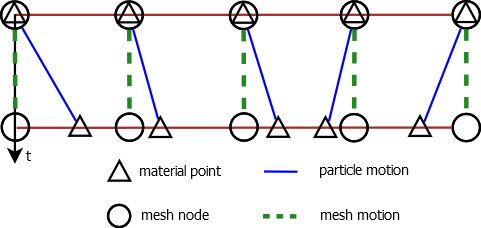
\includegraphics[width=0.8\textwidth]{images/eulerian}
	\caption{Eulerian perspective}
	\label{fig:eulerian}
\end{figure}

A computational mesh can be interpreted as a number of observers distributed across the domain of interest and connected to each other in order to form a a grid with nodes. If the particles of the domain move, a purely euclidean mesh does not move and the position other nodes remain fixed at any instance of time \cite{Cheng2006SlidingFL}. 
This behavior is represented in Figure \ref{fig:eulerian} (adapted from \cite{Cheng2006SlidingFL}). The mesh is independent of particles movement, resulting in a convenient choice for \acrfull{cfd} problems, where fluid flows throughout the whole
computational domain. Within this approach, proper mesh refinement is crucial for computational accuracy as it defines to what extent small scale movement can be modeled and resolved \cite{donea2017arbitrary}.

\subsection{Lagrangian perspective}
\label{subsec:lagrange}

A \textit{lagrangian observer} focuses on a single particles and follows it throughout the motion, as depicted in Figure \ref{fig:lagrangian}. Changes in the quantities of interest are observed at different spatial locations. 

\begin{figure}[htbp!]
	\centering
	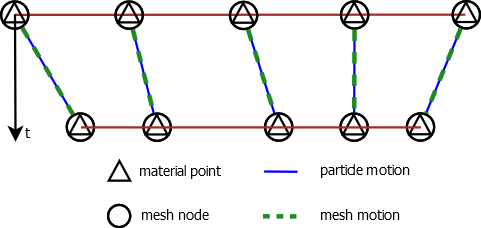
\includegraphics[width=0.8\textwidth]{images/lagrangian}
	\caption{Lagrangian perspective}
	\label{fig:lagrangian}
\end{figure}

The motion of the particle and the other quantities of interest can be described by reference coordinates (or \textit{material coordinates}) in Euclidean space $(X, Y, Z)$, uniquely identifying the observed particle at a reference configuration \cite{XING201957}. Usually $t = 0$ is chosen as reference but this is not mandatory. The Lagrangian observer only registers changes concerning one specific particle as time advances. Thus, quantities of interest can be described as:

\begin{equation}
	\Theta = \hat{\Theta}(X, Y, Z, t)
\end{equation}

In contrast to the Eulerian perspective (Equation \ref{eq:eulerian}), the obtained information is strictly limited to a single material particle (implied by the usage of the capital reference coordinate variables). 
Information about a fixed point in space is not directly available and no convective fluxes appear in a Lagrangian description.

This perspective is again translated into computational meshes: at a reference instance of time, mesh nodes are attached to material particles. As these move, the mesh nodes move with them causing the mesh to deform. Figure \ref{fig:lagrangian} describes the situation. The mesh nodes always coincide with their respective particles.

In this situation large-scale and irregular motions and more importantly deformation lead to distortions of the computational mesh, which yields smaller accuracy in simulations requiring to apply techniques to keep the desired accuracy \cite{lipton2010robustness}.

Lagrangian perspective is the usual method of choice for \acrfull{csm} simulations.

Eulerian and Lagrangian descriptions are related \cite{bertram2012elasticity}. A mapping between them can described by the \textit{motion} function $\phi$ such that:


\begin{equation}
\vec{x}(t) = \phi(\vec{X}, t)
\label{eq:lag-motion}
\end{equation}

Equation \ref{eq:lag-motion} tells that he Eulerian, spatial position $\vec{x}$ of a particle at time t is the
mapping of the particle at its reference configuration $\vec{X}$: the mapping must be bijective.

\subsection{ALE method}
\label{subsec:ALE}

As outlined above, CSM and CFD problems adopt different perspectives. The \acrfull{ale} approach, a combination of the two points of view, is used for FSI problems. As the name implies, an ALE observer moves arbitrarily with respect to a specific material particle.
Figure \ref{fig:ale} depicts such a situation.

\begin{figure}[htbp!]
	\centering
	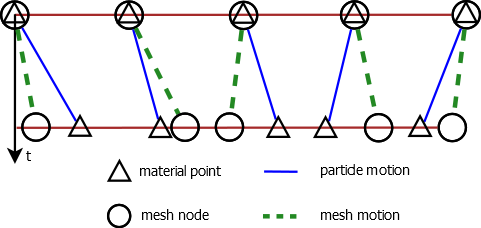
\includegraphics[width=0.8\textwidth]{images/ale}
	\caption{ALE perspective}
	\label{fig:ale}
\end{figure}

When dealing with computational meshes, an ALE mesh is considered as it can move almost arbitrarily with respect to the motion of the underlying particles, as shown in Figure \ref{fig:ale-mesh}.
The only constraint is that node movements should not distort the mesh too much as this leads to computational inaccuracy. Many algorithm exist to implement suitable quality criteria and keep the mesh motion reasonable and to allow the nodes to follow moving particles up to a certain extent \cite{de2007mesh}.

Since the mesh motion and material particle motion are not directly linked, a new unknown is introduced:  the relative movement between the ALE mesh and the material domain. This approach is particularly useful in FSI problems: fluid and solid must follow the moving interface between them for physical reasons.
Since the solid domain is usually described in a Lagrangian perspective, the solid mesh is kept attached to the FSI interface. However, also the fluid domain must deform to avoid formation of gaps between the meshes. Therefore, in ALE methods the fluid mesh nodes at the interface move with it. Fluid mesh nodes follow the fluid particles sticking to the interface (for viscous flows), while the rest of the fluid mesh is allowed to move in such way that mesh distortions are kept minimal, to preserve computational accuracy \cite{ramm1998fluid}.

\begin{figure}[htbp!]
	\centering
	\begin{subfigure}{.5\textwidth}
		\centering
		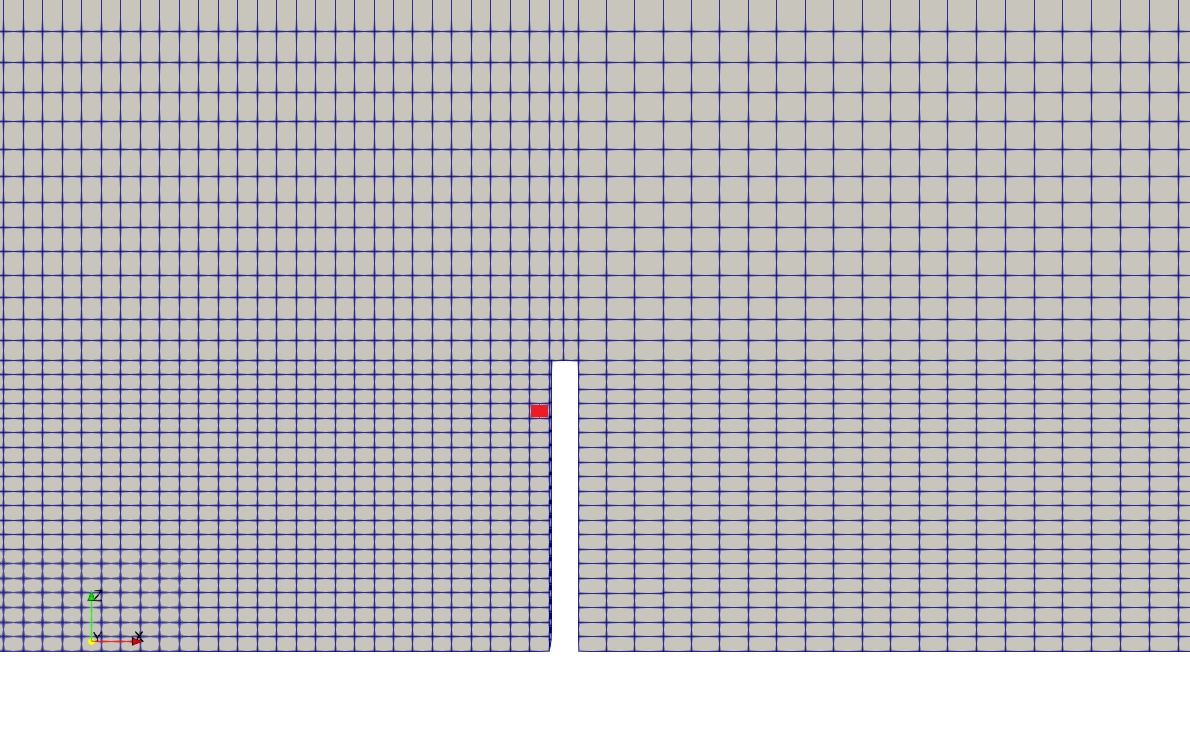
\includegraphics[width=.99\linewidth]{images/undist}
		\caption{undistorted mesh}
		\label{fig:undist}
	\end{subfigure}%
	\begin{subfigure}{.5\textwidth}
		\centering
		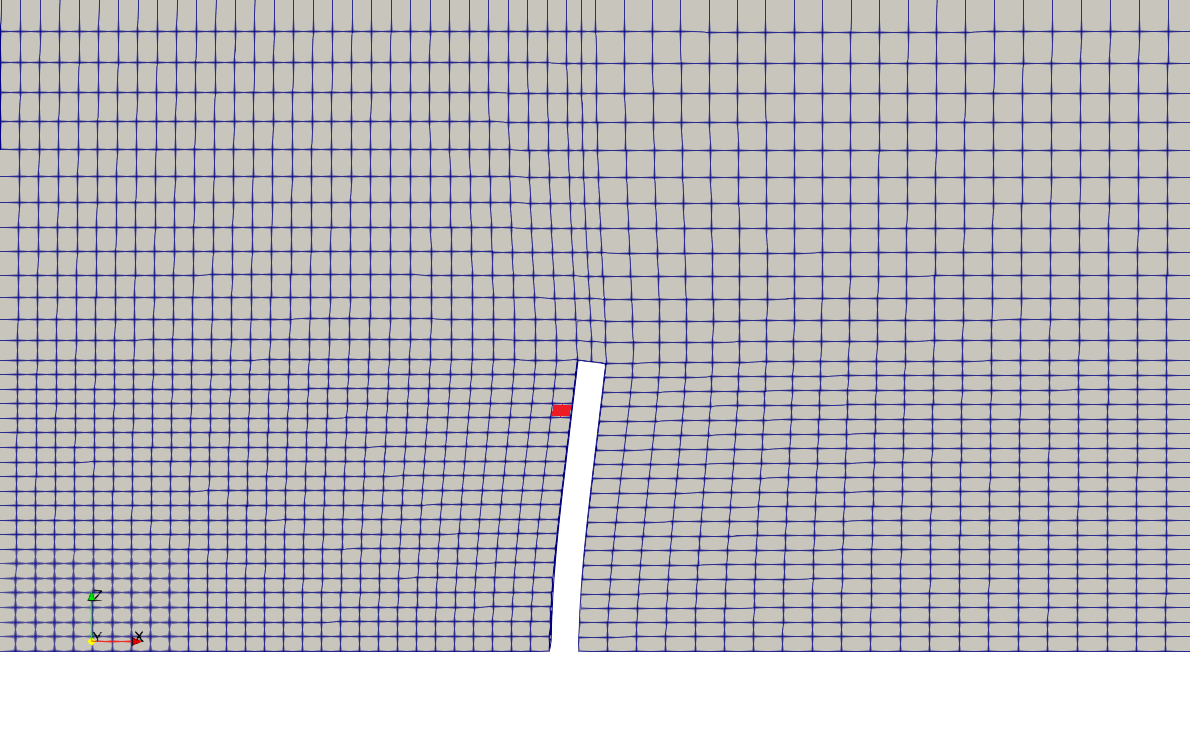
\includegraphics[width=.99\linewidth]{images/dist}
		\caption{distorted mesh}
		\label{fig:dist}
	\end{subfigure}
	\caption{ALE mesh}
	\label{fig:ale-mesh}
\end{figure}

\section{Domains and interface}
\label{sec:models}

Fluid-structure interaction implies that the overall model is determined by models defining the fluid behavior and the solid behavior, briefly described in sections \ref{sec:solid} and \ref{sec:fluid}. A short overview of beam models is given in section \ref{sec:beam} as it is relevant for the model developed in this work.
Finally a formal definition of the interface is given in section \ref{sec:interface}, as it is necessary to define suitable coupling conditions at the common boundary of the solid and the fluid.


\subsection{Fluid domain}
\label{sec:fluid}

An exhaustive description of all possible fluid models is far beyond the scope of this work. A quite general model is the viscous compressible one described by the \acrfull{nse}. 

\begin{subequations}
\begin{eqnarray}
	\label{eq:cont}
	\frac{\partial{\rho}}{\partial{t}} + \nabla \cdot \left(\rho \vec{v}\right) &=&  0 \\	
	\label{eq:mom-cons} 
	\frac{\partial }{\partial t}\left( \rho \vec{v} \right) + \nabla \cdot \left( \rho \vec{v} \otimes \vec{v} \right) +\nabla p - \nabla \cdot \mathbf{\tau} - \rho \vec{g} &=& 0 \\
	\label{eq:energy-cons}
	\frac{\partial }{\partial t}\left( \rho e_0  \right) + \nabla \cdot \left( \rho e_0 \vec{v} \right) + \nabla \cdot \left( \vec{v}p + \vec{q} -\vec{v} \cdot \bm{\tau} \right) - \vec{v} \cdot \rho \vec{g} &=& 0
\end{eqnarray}
\end{subequations}

where:
\begin{itemize}
	\item $\rho$ denotes density
	\item $\vec{v}$ is flow velocity in all dimensions
	\item \textit{p} denotes pressure
	\item $\bm{\tau}$ is the viscous stress tensor
	\item $\vec{g}$ represents the sum of all body forces
	\item $e_0$ is the total energy per unit mass
	\item $\vec{q}$ is the heat flux by conduction
\end{itemize}

They consist in the mass conservation equation (\ref{eq:cont}), the conservation of momentum equation (\ref{eq:mom-cons}) and the energy conservation equation (\ref{eq:energy-cons}). For a Newtonian fluid, the viscous stress tensor is given by:

\begin{equation}
	\label{eq:tau}
	\bm{\tau} = -\frac{2}{3}\mu \left( \nabla \cdot \vec{v} \right) I +2\mu S
\end{equation}

with $\mu$ being the dynamic viscosity and \textit{S} the rate of deformation tensor (i.e. the symmetric part of the velocity gradient $\nabla \vec{v}$):

\begin{equation}
	\label{eq:def_tens}
	\mathbf{S} = \frac{1}{2} \left( \nabla \vec{v} + \nabla \vec{v}^T \right)
\end{equation}

A detailed derivation of such equations and the theory beyond can be found for example in  \cite{quartapelle2013fluidodinamicaI} and \cite{quartapelle2013fluidodinamicaC} or in \cite{pope2001turbulent}. 

The set of equations above, even with a Newtonian fluid model, lack some other information in order to form a closed set of \acrfull{pde}. A conductive heat flux model is needed  (e.g. Fourier’s Law), the caloric and thermodynamic equations of state have to be chosen, a proper turbulence model if needed (see \cite{pope2001turbulent}) and finally, the appropriate initial and boundary conditions for the problem \cite{galdi2011introduction} must be defined.

Simplifications can be done to obtain less sophisticated models such as: adiabatic, inviscid, incompressible, and many others. Dimensional Analysis is a powerful tool to determine to what extent some reduced models are meaningful, and it is widely used in fluid dynamics, as described in section \ref{sec:dimensional}. Most CFD software codes allow to set up simulations with the most suitable model which can be coupled with a solid model to build a FSI problem. Some further details are given in section \ref{sec:monolithic}. 


\subsection{Solid domain}
\label{sec:solid}

In solid mechanics, particles do not travel as much as they do in fluid dynamic problems, as described in \ref{subsec:lagrange}. For this reason, a Lagrangian perspective is generally used.  

The  de-Saint Venant-Kirchhoff model \cite{ogden1997non} is very commonly used when describing the movement of a solid: it is also often used in FSI problems ad it is capable of handling large deformation. The material is considered:

\begin{itemize}
	\item \textit{homogeneous}: the material properties do not depend on the position of the particle
	\item \textit{linear elastic}: the stress-strain relationship is linear
	\item \textit{isotropic}: the stress-strain relationship is independent from the direction of the load
\end{itemize}

A general expression of the dynamic equation can be derived from the \acrfull{vwp} applied to an arbitrary control volume: 

\begin{equation}
	\label{eq:mech}
	\frac{\partial^2 \vec{u} }{\partial t^2} = \nabla \cdot \mathbf{T} + \rho \vec{f}
\end{equation}

In equation \ref{eq:mech}:

\begin{itemize}
	\item $\rho$: is the material density
	\item $\vec{u}$: is the particle displacement
	\item $\mathbf{T}$: is the \textit{second Piola-Kirchhoff} stress tensor
	\item $\vec{f}$: is the sum of body forces
\end{itemize}


In order to close the dynamic equation, a constitutive law which must be considered to relate stress and strain:

\begin{equation}
	\mathbf{T} = \lambda \mathbf{I} \mathrm{tr}\left[ \bm{\varepsilon_G}  \right]  + 2\mu \bm{\varepsilon_G}
\end{equation}

where $\bm{\varepsilon_G}$ is the Green-Lagrange strain tensor:

\begin{equation}
	\bm{\varepsilon_G} = \frac{1}{2}\left( \mathbf{F}^T \mathbf{F}-\mathbf{I}  \right)
\end{equation}

and $\mathbf{F}$ is the deformation gradient. $\lambda$ and $\mu$ are material properties and are named Lamé constants. These relate to the Young modulus \textit{E} and the Poisson ratio $\nu$ which are more commonly used in practice. The relationship among the various parameters is the following:


\begin{eqnarray}
	E &=& \frac{\mu(3\lambda+2\mu)}{\lambda + \mu} \\
	\nu &=& \frac{\lambda}{2(\lambda + \mu)}
\end{eqnarray}

The set of parameters $\left(E, \nu\right)$ or $\left(\lambda, \mu \right)$, together with the density $\rho$ fully define the material, under the assumptions of linear elasticity, isotropy and homogeneity.

The set of PDEs is completed when suitable initial and boundary conditions are defined.

\subsection{Models with reduced dimensionality: beams}
\label{sec:beam}

The equations introduced in section \ref{sec:solid} may be a tough task to solve even of the case of isotropic hyperelasticity, when considering a 3-D domain. Even with today's computers and using finite elements techniques, it is not always feasible or convenient to treat a solid as a three-dimensional continuum. Body with particular geometric features can be seen as lower dimension bodies, with respect to the governing equations \cite{hjelmstad2007fundamentals}. Such bodies are called \textit{beams} (one dimension) , \textit{plates} or \textit{shells} (two dimensions).

The \textit{beam} model splits the description of the geometry into two subproblems:
\begin{enumerate}
	\item a beam is defined by its \textit{reference line} and the movement (displacement and rotation) of the solid is completely defined by it (see Figure \ref{fig:beam-model}),
	\item the beam \textit{cross section} is considered as a whole, its movement depends on the movement of the reference line, stresses are generalized into \textit{resultants} (axial, bending, shear, torsional) which represent the aggregate effect of all of the stresses acting on the cross section. The constitutive properties of the section (axial, shear, torsion and bending stiffness) allow to relate stresses and deformations (by means of VWP) and close the problem.
\end{enumerate}


\begin{figure}[htbp!]
	\centering
	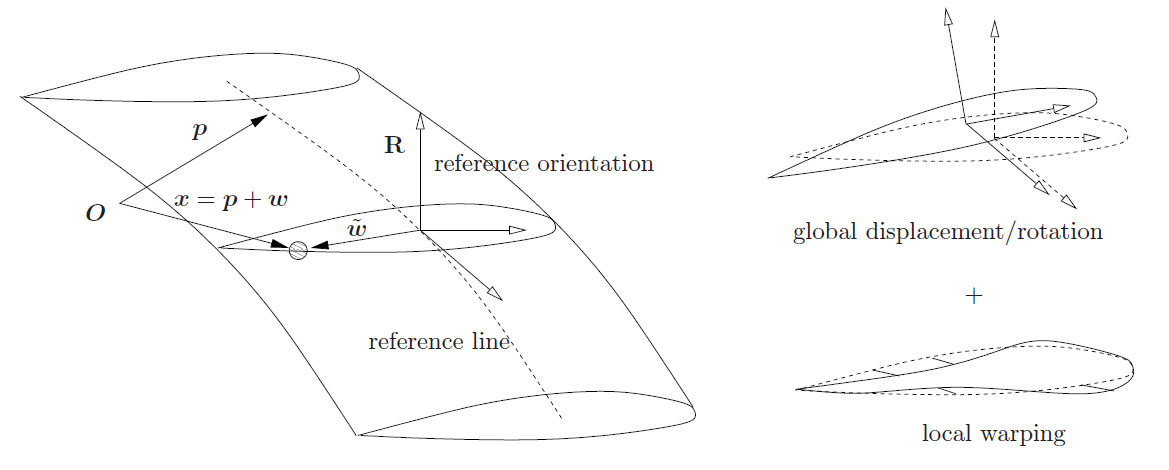
\includegraphics[width=0.8\textwidth]{images/beam}
	\caption{beam model, taken from \cite{ghiringhelli2008integrated}}
	\label{fig:beam-model}
\end{figure}


The beam model can be used to build elements of a \acrfull{fem}. For example, the beam element can be modeled by means of a Finite Volume approach, as described in \cite{ghiringhelli2000multibody}, which computes the internal forces as functions of the straining of the reference line and orientation at selected points along the line itself, called evaluation points.

This approach is particularly interesting for \acrshort{fsi} problems in which slender structures are involved. A mapping is needed between the fluid-solid interface and the reference line movement, which will be described in Sections \ref{sec:mbd-beam} and \ref{sec:mbd-forces}.


\subsection{Interface and interaction}
\label{sec:interface}

Since \acrshort{fsi} problems are centered on the interaction of the fluid and solid domain, their common interface needs to be described properly. A simple representation of the situation at the so called \textit{wet surface} is shown in Figure \ref{fig:interface}. Quantities related to the solid use S subscript, while fluid domain and the interface are labeled with F and FS, respectively. 

\begin{figure}[htbp!]
	\centering
	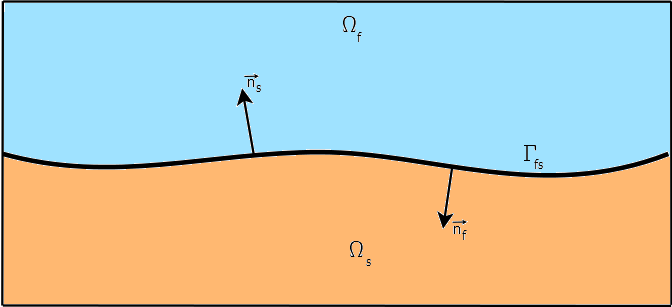
\includegraphics[width=0.8\textwidth]{images/interface}
	\caption{fluid solid interface}
	\label{fig:interface}
\end{figure}

In order to have a physically correct behavior, some conditions have to be met \cite{hou2012numerical}:

\begin{itemize}
	\item solid and fluid domains should not overlap nor separate,
	\item for a viscous fluid model, the flow velocity at the interface must equal the boundary velocity (\textit{no-slip} condition),
	\item for an inviscid fluid model, only velocity components normal to the wet surface have to be equal to the structural 	velocity as the fluid may slip freely in tangential direction at any boundary,
	\item forces exchanged at the interface must at equilibrium.
\end{itemize}

The first conditions result in the \textit{kinematical requirement} that the displacements of fluid and solid domains, as well as their respective velocities have to be equal at the wet surface (denoted by $\Gamma_{FS}$): 

\begin{eqnarray}
 \Delta\vec{x}_F &=& \vec{u}_S \\
 \vec{v}_F &=& \frac{\partial \vec{u}_S}{\partial t}
\end{eqnarray}

The last condition results in the equilibrium requirement. Force vectors are computed from the stresses at the interface and the outward normal vectors of fluid and solid domain, respectively. They have to be equal and opposite leading to the dynamic coupling condition:

\begin{equation}
\bm{\sigma_F} \cdot \vec{n}_F + \bm{\sigma_S} \cdot \vec{n}_F = 0
\end{equation}

$\bm{\sigma} \in \mathbb{R}^{3 \times 3}$ represents the stress tensor (note that for the fluid it comprises pressure and viscous stresses), while $\vec{n} \in \mathbb{R}$ is the outward normal unit vector.


\section{Classification of FSI problems}
\label{sec:classification}

In the previous chapters we have seen that there exist a lot of models that can describe fluid flow and solid mechanics. In FSI problems we need to couple two of them: the variety of coupled problems seems to be so large that  single FSI model that is applicable to every problem appears to be unfeasible. For this reason it is useful to classify FSI problems and look for specific properties in each class.  
The first step is to switch from dimensional quantities to dimensionless ones.


\subsection{Dimensional analysis}
\label{sec:dimensional}

We use the principle that a physical law should only relate to dimensionless quantities.  
There exist a rather general theorem called the $\Pi$ Theorem or the \textit{Vaschy-Buckingham Theorem} \cite{HancheOlsen2004}, which tells how many dimensionless quantities are needed to rewrite a model in dimensionless fashion.
This theorem states that the number of dimensionless quantities, P, is equal to that of the dimensional ones describing the problem, N, minus R, which is the rank of the matrix of dimension exponents. This matrix is formed by the columns of the dimension exponents of all variables \cite{hardtke2019buckingham}. An example is given in the following Section \ref{sec:dim-fluid}, Table \ref{table:dim-fluid}.

\subsection{Dimensional analysis in fluid domain}
\label{sec:dim-fluid}

Dimensional analysis is widely used in fluid dynamics. In order to keep the analysis simple,, we consider the adimensionalization of the incompressible Navier-Stokes momentum equation for a Newtonian fluid \cite{fox2020fox}:

\begin{equation}
	\frac{\partial \vec{v}}{\partial t} + \left(\vec{v} \cdot \nabla \right) \vec{v} = -\frac{\nabla p}{\rho} + \nu \nabla ^2 \vec{v} + \vec{g}
	\label{eq:inc-ns}
\end{equation}

The variables involved in equation \ref{eq:inc-ns} are the following:

\begin{itemize}
	\item \textit{t}: time
	\item $\vec{x}$: coordinates
	\item $\vec{v}$: velocity field
	\item \textit{p}: pressure field
	\item $\rho$: fluid density
	\item $\nu$: fluid kinematic viscosity
	\item $\vec{g}$: gravity
	\item \textit{L}: reference dimension
	\item $V_0$: reference velocity
\end{itemize}




\begin{table}[!h]
\begin{center}
	\begin{tabular}{ c|c c c c c c c c c} 
		  & \textit{t} & $\vec{x}$ & $\vec{v}$ & \textit{p} & $\rho$ & $\nu$ & $\vec{g}$ & \textit{L} & $V_0$  \\ 
		\hline
		L & 0 & 1 & 1  & -1 & -3 & 2  & 1  & 1 & 1  \\ 
		M & 0 & 0 & 0  &  1 &  1 & 0  & 0  & 0 & 0  \\
		T & 1 & 0 & -1 & -1 &  0 & -1 & -2 & 0 & -1 \\ 
	\end{tabular}
\end{center}
\caption{fluid  matrix of dimension exponents}
\label{table:dim-fluid}
\end{table}

The rank of the above matrix is 3 so 6 dimensionless parameters are needed to rewrite the equation \ref{eq:inc-ns}:

\begin{itemize}
	\item \textit{length}: $\vec{x}^* = \frac{\vec{x}}{L}$
	\item \textit{velocity}: $\vec{v}^* = \frac{\vec{v}}{V_0}$
	\item \textit{time}: $t^* = \frac{V_0 t}{L} = \frac{t}{T_{fluid}}$
	\item \textit{pressure}: possible choices: $p^* = \frac{p}{\rho V_0^2}$ or, if viscous forces are dominant, $p*= \frac{p L}{\rho \nu V_0}$
	\item \textit{Reynolds number}: $Re=\frac{V_0 L}{\nu}$. It defines the ratio between inertia and viscous forces.
	\item \textit{Froude number}: $Fr = \frac{V_0}{\sqrt{g L}}$. It defines the ratio between the flow inertia to the body field forces
\end{itemize} 


The adimensionalized momentum equation becomes:

\begin{equation}
	\frac{\partial \vec{v}^*}{\partial t^*} + \left( \vec{v}^* \cdot \nabla \right) \vec{v}^* = -\nabla p^* +\frac{1}{Re} \nabla^2 \vec{v}^2 + \frac{1}{Fr^2}\vec{g}
	\label{eq:adim-ns}
\end{equation}

From Equation \ref{eq:adim-ns} a lot of models might be derived: from \textit{Stokes regime} when viscosity is dominant, to \textit{Euler regime} when viscosity is negligible with respect to inertia forces.


\subsection{Dimensional analysis in solid domain}

Even if it is seldom used, Dimensional Analysis can be made also for the solid domain \cite{longo2011analisi}.

The variables involved in a solid dynamics equation are:

\begin{itemize}
	\item \textit{t}: time
	\item $\vec{X}$: coordinates
	\item $\vec{u}$: displacement field
	\item $\rho_S$: solid density
	\item \textit{E}: elastic modulus
	\item $\vec{g}$: gravity
	\item \textit{L}: reference dimension
	\item $U_0$: reference displacement
\end{itemize}

From the variables above the following parameters can be derived:

\begin{itemize}
	\item \textit{length}: $\frac{\vec{X}}{L}$: dimensionless coordinate
	\item \textit{displacement}: $\frac{\vec{u}}{L}$: dimensionless displacement
	\item \textit{time}: $\frac{t \sqrt{\frac{E}{\rho_S}}}{L} = \frac{t}{T_{solid}}$ dimensionless time
	\item entity of displacements: $\frac{U_0}{L} = \delta$: \textit{displacement number}
	\item gravity: $\frac{\rho_S g L}{E}$: elastogravity number
\end{itemize}

$T_{solid}$ can be seen as $\frac{L}{c}$ with $c = \sqrt{\frac{E}{\rho_S}}$ which is the scale of elastic wave velocity. The displacement number $\delta$ tells how big the structure displacement are related to the overall dimension, and defines the \textit{large displacements} region.
Finally, the \textit{elastogravity number} combines gravity (or body forces in general), density and stiffness: when large the deformation induced by body forces in the solid are large. 

\subsection{Dimensional analysis of coupled problems}

It is now possible to undertake the dimensional analysis of a fully coupled fluid and solid interaction problem. Some of the parameters are only defined in the fluid side or in the solid side (e.g. viscosity or stiffness). Some parameters are common to both domains (e.g. length scale or gravity). The variables of interest are now the velocity in the fluid and the displacements in the solid. Each of them can be related to all the parameters without separation. For example, the fluid velocity relationship is of the kind:

\begin{eqnarray}
	 g(\vec{v}; \vec{x},t; \rho, \mu, V_0; \rho_S. E; \vec{g}, L) = 0
	 \label{eq:vel-param}
\end{eqnarray}


Equation \ref{eq:vel-param} is composed of 11 dimensional parameters. Applying $\pi$ theorem, the total number of independent dimensionless parameter expected is 8. Starting from the ones derived in the previous sections:

\begin{enumerate}
	\item $\vec{x}^* = \frac{\vec{x}}{L}$: dimensionless coordinates
	\item $\vec{v}^* = \frac{\vec{v}}{V_0}$: dimensionless fluid velocity
	\item $t*_f = \frac{V_0 t}{L}$: dimensionless time
	\item $Re = \frac{V_0 L}{\nu}$: Reynolds number
	\item $Fr = \frac{V_0}{\sqrt{gL}}$: Froude number
	\item $\delta = \frac{U_0}{L}$: displacement number
	\item $\frac{\rho_S g L}{E}$: elastogravity number
\end{enumerate}

The 7 quantities above derive from the separated problem. The last one necessarily mixes things from the fluid and the solid side otherwise it would have been found in one uncoupled case. There is no unique choice for this parameter, the following are the most common ones.

\subsubsection{Mass number}
\label{subsec:mass-ratio}

The simplest, but arguably most important parameter is the ratio of the two densities: the \textit{Mass Number} M.

\begin{equation}
	M = \frac{\rho}{\rho_S}
	\label{eq:mass-number}
\end{equation}

This can range from $\mathcal{O}\left(10^{-4}\right)$ in air-steel interaction to $\mathcal{O}\left(1\right)$ when both media have about the same density. This parameter is particularly significant for the so called \textit{added mass} stability problem, described in Section \ref{sec:added-mass}.

\subsubsection{Reduced velocity}

Another possible choice is the reduced velocity:

\begin{equation}
	 U_R = \frac{V_0}{\sqrt{\frac{E}{\rho_S}}}
\end{equation}

It is the ratio between the fluid free velocity and the velocity of elastic waves in a solid, \textit{c}. It contains information on the way the two dynamics are related and it can range different orders of magnitude.

\subsubsection{Cauchy number}

Another possible parameter combines stresses or stiffness: the  Cauchy number, as defined in \cite{de2001fluides}:

\begin{equation}
	C_Y = \frac{\rho V_0^2}{E}
\end{equation}

It is the ratio between the fluid inertial forces, quantified by the dynamic pressure and the stiffness of the solid E. 
The higher it is, the more the solid is elastically deformed by the flow.


These are actually the most important parameters involving FSI problems. Among them, there is no universally better choice. But there are efficient choices, that would be more helpful
in solving a given problem. 



\chapter{Computational aspects of Fluid-Structure Interaction problems}
\label{cha:computation}

This section deals with the computational aspects of FSI problems. The first possible categorization of solution techniques distinguishes between monolithic and partitioned approach, as discussed in Section \ref{sec:monolithic}. This work is based on the latter approach, so the two different coupling strategies, namely strong and weak, are discussed in Section \ref{sec:coupling}. As strong coupling is generally needed for accurate solution, ad overview of strong coupling algorithms is given in Section \ref{sec:strong-coupling}. Section \ref{sec:interface-mesh} focuses on aspects concerning the interface mesh, and how the solid and the fluid exchange data between them. Finally \ref{sec:addedd-mass} briefly describes a common issue arising in strongly coupled problems: the ~\ac{AME}.


\section{Monolithic and Partitioned Approach}
\label{sec:monolithic}

Analytical solutions are impossible to obtain for the large majority of FSI problems; on the other hand, laboratory experiments may be costly, unfeasible or limited. For those reasons, numerical simulations may be employed to analyze the physics involved in the interaction between fluids and solids. With the current capabilities of computer technology, simulations of scientific and engineering models have become increasingly detailed and sophisticated.

The numerical methods used to solve FSI problems may be roughly classified into two classes: the \textit{monolithic approach} and the \textit{partitioned approach}. There is no exact distinction between the two approaches, as they might be seen differently among fields of applications. The idea here is to consider how many solvers are used to find a solution.

In the \textit{monolithic approach}, the whole problem is treated as a unique entity and solved simultaneously with a specialized ad hoc solver (see Figure \ref{fig:monolithic}). The fluid and structure dynamics form a single system of equations for the entire problem, which is solved simultaneously by a unified algorithm. The interface conditions are implicit in the solution procedure \cite{hubner2004monolithic}, \cite{ryzhakov2010monolithic}.

This approach can potentially achieve better accuracy, as they solve the system of equations exactly the interface conditions are implicit in the model \cite{richter2017fluid}, but it may require more resources and expertise to develop from scratch a specialized code (it solves a very specific model) that can be cumbersome to maintain.

\begin{figure}[htbp!]
	\centering
	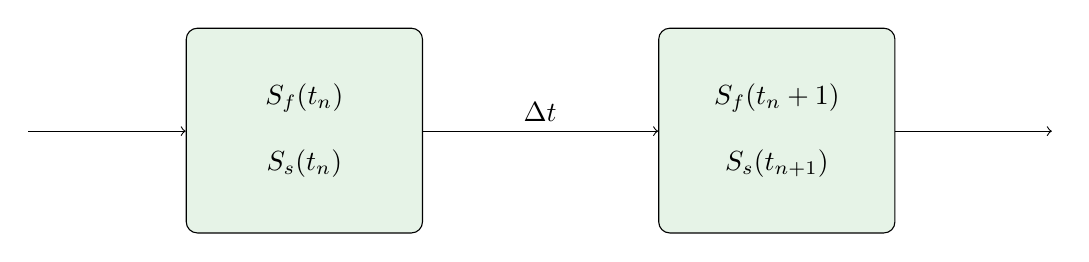
\begin{tikzpicture}[scale=1]


	\tikzstyle{status}=[draw,rectangle,rounded corners,fill=green!10,text centered,inner sep=10pt, anchor=south west, minimum width=3cm,minimum height=2.6cm]
	\draw[->] (0,1.3)-- (2,1.3) node[] {};
	
	\draw[->] (5,1.3)-- (8,1.3) node[midway,above] {$\Delta t$}; % node[midway,below] {step};

	\draw[->] (11,1.3)-- (13,1.3) node[] {};

	\node[status] (t1) at (2,0)  {
		\begin{tabular}{c}
			$S_f(t_n)$ \\
			\\
			$S_s(t_n)$
	\end{tabular}};

	\node[status] at (8,0) {
	\begin{tabular}{c}
		$S_f(t_{n}+1)$ \\
		\\
		$S_s(t_{n+1})$
\end{tabular}};
	
%		\draw (0,1.3) node[below] {$B$} --
%		(3,1.3) node[below] {$C$} --
%		(1.5,4.3) node[above] {$A$} -- cycle;
%		\draw (1.5,4.3) -- (1.5,1.3) node[below] {$D$};
%		\draw (1.5,1.5) -- (1.7,1.5) -- (1.7,1.3);
%		\node[draw,text width=3cm] at (4.5,4) {some text spanning three lines with automatic line breaks};
%		\draw[rounded corners=5pt] (4,0) rectangle ++(2,1);
	\end{tikzpicture}
	\caption{monolithic approach: $S_f$, $S_s$ denote the fluid and the structure solutions}
	\label{fig:monolithic}
\end{figure}


On the other hand, in the \textit{partitioned approach}, the fluid and the solid domains are treated as two distinct computational fields, with their respective meshes, that have to be solved separately (see Figure \ref{fig:partitioned}: how data are passed between solvers is detailed in Section \ref{sec:coupling}). The interface conditions are used explicitly to communicate information between the fluid and structure solutions. This implies that the flow does not change while the solution of the structural equations is calculated and vice versa \cite{degroote2009performance}. The partitioned approach thus requires a third software module (i.e. a coupling algorithm) to incorporate the interaction aspects. It communicates the boundary conditions described in Section \ref{sec:interface}: that is forces or stresses (dynamic data) calculated by the fluid solver at the wet surface are passed to the solid component and displacements or velocities (kinematic data) computed by the solid solver at the interface are sent to the fluid component in return. Finally, fluid and structural solutions together yield the FSI solution.

\begin{figure}[htbp!]
	\centering
	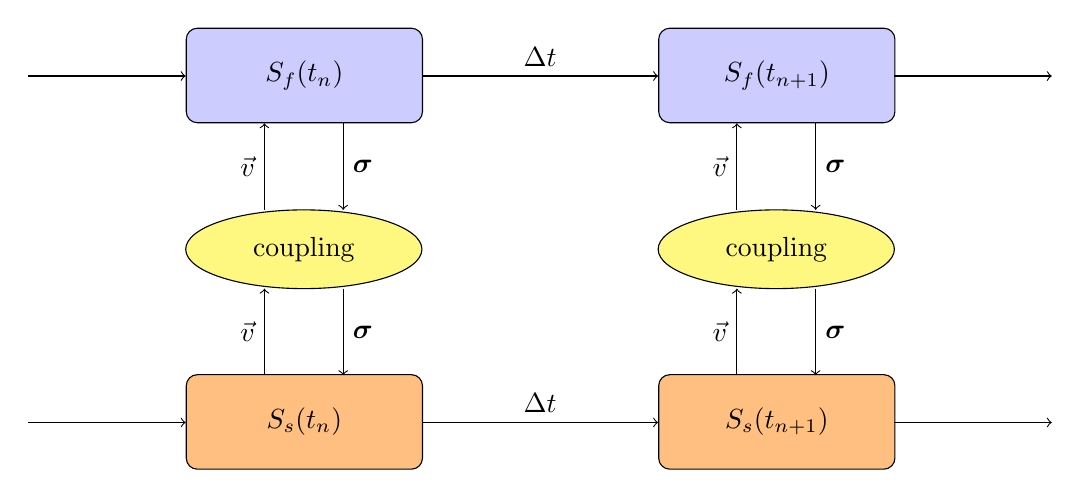
\begin{tikzpicture}[scale=1]

	\tikzstyle{solver}=[draw,rectangle,rounded corners,text centered,inner sep=10pt, anchor=south west, minimum width=3cm,minimum height=1.2cm]
	\tikzstyle{coupling}=[draw, ellipse, fill=yellow!75, minimum width=3cm, minimum height=1.2cm, align=center]

	\node[solver,fill=blue!20] at (2,4.4) {$S_f(t_n)$};
	\node[solver,fill=blue!20] at (8,4.4) {$S_f(t_{n+1})$};
	
	\node[solver,fill=orange!50] at (2,0) {$S_s(t_n)$};
	\node[solver,fill=orange!50] at (8,0) {$S_s(t_{n+1})$};
	
	\draw[->] (0,0.6)-- (2,0.6) node[] {};
	\draw[->] (5,0.6)-- (8,0.6) node[midway,above] {$\Delta t$}; % node[midway,below] {step};
	\draw[->] (11,0.6)-- (13,0.6) node[] {};


	\draw[->] (0,5)-- (2,5) node[] {};
	\draw[->] (5,5)-- (8,5) node[midway,above] {$\Delta t$}; % node[midway,below] {step};
	\draw[->] (11,5)-- (13,5) node[] {};
	
	\node[draw,fill=yellow!50,ellipse,minimum width=3cm, minimum height=1cm] at (3.5,2.8) {coupling};
	\node[draw,fill=yellow!50,ellipse,minimum width=3cm, minimum height=1cm] at (9.5,2.8) {coupling};

	\draw[->] (3,1.2)-- (3,2.3) node[midway,left] {$\vec{v}$};
	\draw[->] (4,2.3)-- (4,1.2) node[midway,right] {$\bm{\sigma}$};

	\draw[->] (3,3.3)-- (3,4.4) node[midway,left] {$\vec{v}$};
	\draw[->] (4,4.4)-- (4,3.3) node[midway,right] {$\bm{\sigma}$};

	\draw[->] (9,1.2)-- (9,2.3) node[midway,left] {$\vec{v}$};
	\draw[->] (10,2.3)-- (10,1.2) node[midway,right] {$\bm{\sigma}$};

	\draw[->] (9,3.3)-- (9,4.4) node[midway,left] {$\vec{v}$};
	\draw[->] (10,4.4)-- (10,3.3) node[midway,right] {$\bm{\sigma}$};
		
	\end{tikzpicture}
	\caption{partitioned approach: $S_f$, $S_s$ denote the fluid and the structure solutions, while $\bm{\sigma}$ and $\vec{v}$ represent coupling data}
	\label{fig:partitioned}
\end{figure}

A big advantage of this approach is that software modularity is preserved: different and efficient solution techniques can be used for the flow equations and structural equations. Provided that they can exchange data, existing solvers for the fluid and solid problem can be reused, ranging from commercial to academic and open-source codes. Those solvers are usually well-validated.
Besides, compared to monolithic procedures, the programming efforts are lower for partitioned approaches, as only the coupling of the existing solvers has to be implemented rather than the solvers themselves.
The challenge of this approach is, however, to define and implement algorithms to achieve accurate and efficient fluid-structure interaction solution with minimal code modification. Particularly, the interface
location that divides the fluid and the structure domains changes in time. The partitioned approach requires that the fluid solver has ALE capabilities, as introduced in Section \ref{subsec:ALE}.
More detailed and practical explanations about the coupling component used in this work are given in Section \ref{sec:precice}. 


\section{Coupling Strategies}
\label{sec:coupling}

Because of the modularity, the partitioned approach has gained much attention in research. The structure sketched in Figure \ref{fig:partitioned} needs to be detailed and specialized in function of the coupling strategies.

In an interface multi-physics coupling like FSI, the boundary surface is in common between the two sides of the simulation. The results make sense and are numerically stable only if the two sides of the interface are in agreement, since the output values of the one simulation become input values for the other (and vice-versa).
The solution strategies can be roughly divided into weakly and strongly coupled approaches. They are often referred to as \textit{explicit} and \textit{implicit} methods in the literature.
When the fluid and solid solutions are computed iteratively until some convergence criteria within the same time step, the scheme is called \textit{implicit coupling}. The faster, simpler but less precise \textit{explicit coupling} consists in executing a fixed number of iterations (typically one per time step) and exchange coupling values without convergence checks. 

\subsection{Explicit coupling schemes}

As in the previous Section, $S_f$ represents the fluid solver, which computes the pressures (named $d_f$ here) at the deformable boundary and $S_s$ is the structure solver, which uses these forces to compute the displacement and velocity of the boundary (named $d_s$). In a \textit{serial-explicit} (or \textit{conventional staggered}) coupling scheme, the solver $S_f$ uses the old time step boundary values $d_s^{(n)}$ to compute the values of $d_f^{(n+1)}$ for the next time step:

\begin{equation}
	d_f^{(n+1)} = S_f\left(d_s^{(n)}\right)
	\label{eq:stag1}
\end{equation}

When the fluid solver completes the time step, data are passed to the structural solver:

\begin{equation}
	d_s^{(n+1)} = S_s\left( d_f^{(n+1)} \right)
	\label{eq:stag2}
\end{equation}

Note that Equation \ref{eq:stag1} uses values computed at $t^n$, while Equation \ref{eq:stag2} uses values computed at $t^{(n+1)}$. The order of execution might be inverted.

In order reduce execution time, the solvers might run in parallel, using data from the same time step (\textit{parallel-explicit coupling}:

\begin{subequations}
\begin{eqnarray}
	d_f^{(n+1)} &=& S_f\left(d_s^{(n)}\right) \\
	d_s^{(n+1)} &=& S_s\left( d_f^{(n)} \right)
	\label{eq:par-exp}
\end{eqnarray} 
\end{subequations}


The two explicit schemes are shown schematically in Figures \ref{fig:serial-explicit} and \ref{fig:parallel-explicit}.

\begin{figure}[htbp!]
	\centering
	\begin{subfigure}{.8\textwidth}
	\centering
	% include first image
		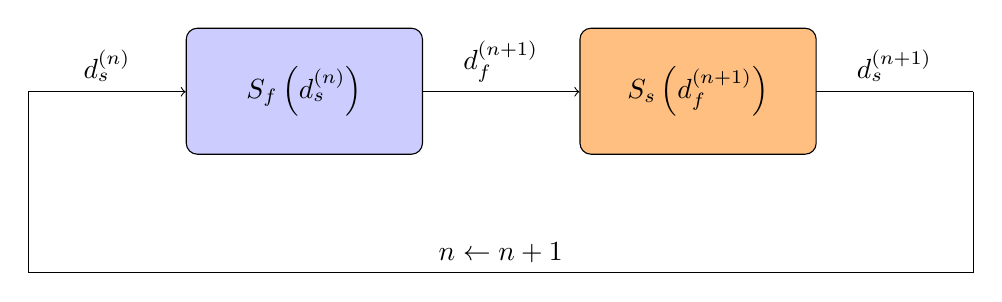
\begin{tikzpicture}[scale=1]
		\tikzstyle{solver}=[draw,rectangle,rounded corners,text centered,inner sep=10pt, anchor=south west, minimum width=3cm,minimum height=1.6cm]
		
		\node[solver,fill=blue!20] at (3,5) {$S_f\left( d_s^{(n)} \right)$};
		\node[solver,fill=orange!50] at (8,5) {$S_s\left(d_f^{(n+1)}\right)$};
		
		\draw[->] (1,5.8)-- (3,5.8) node[midway,above] {$d_s^{(n)}$};
		\draw[->] (6,5.8)-- (8,5.8) node[midway,above] {$d_f^{(n+1)}$};
		\draw[-] (11,5.8)-- (13,5.8) node[midway,above] {$d_s^{(n+1)}$};
		
		\draw[-] (13,5.8)-- (13,3.5);
		\draw[-] (1,5.8)-- (1,3.5);
		
		\draw[-] (1,3.5)-- (13,3.5) node[midway,above] {$n \leftarrow n+1$};
		
		\end{tikzpicture}
		\caption{serial explicit coupling}
		\label{fig:serial-explicit}
	\end{subfigure}
	\newline
	\centering
	\begin{subfigure}{.8\textwidth}
	\centering
	% include second image
		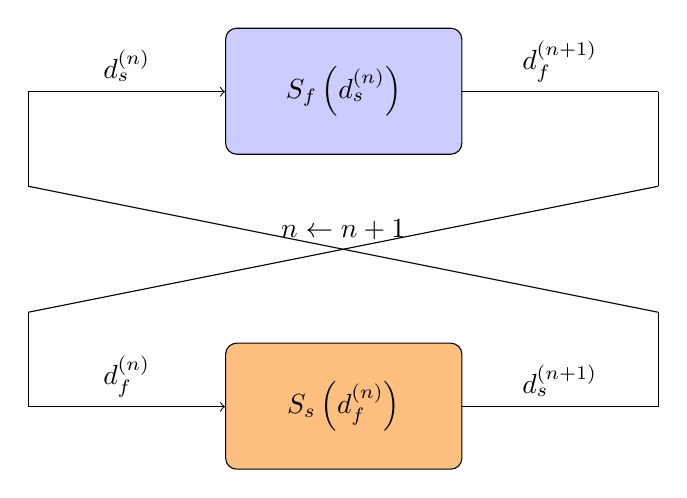
\begin{tikzpicture}[scale=1]
		\tikzstyle{solver}=[draw,rectangle,rounded corners,text centered,inner sep=10pt, anchor=south west, minimum width=3cm,minimum height=1.6cm]

		\node[solver,fill=blue!20] at (2.5,4) {$S_f\left( d_s^{(n)} \right)$};
		\node[solver,fill=orange!50] at (2.5,0) {$S_s\left(d_f^{(n)}\right)$};
		
		\draw[->] (0,4.8)-- (2.5,4.8) node[midway,above] {$d_s^{(n)}$};
		\draw[->] (0,0.8)-- (2.5,0.8) node[midway,above] {$d_f^{(n)}$};

		\draw[-] (5.5,4.8)-- (8,4.8) node[midway,above] {$d_f^{(n+1)}$};
		\draw[-] (5.5,0.8)-- (8,0.8) node[midway,above] {$d_s^{(n+1)}$};
		
		\draw[-] (0,0.8)-- (0,2);
		\draw[-] (8,0.8)-- (8,2);
		
		\draw[-] (0,3.6)-- (0,4.8);
		\draw[-] (8,3.6)-- (8,4.8);
		
		\draw[-] (8,3.6)-- (0,2) node[midway,above] {$n \leftarrow n+1$};
		\draw[-] (0,3.6)-- (8,2);

	
		\end{tikzpicture}
		\caption{parallel explicit coupling}
		\label{fig:parallel-explicit}
	\end{subfigure}
	\caption{Explicit coupling schemes}
\end{figure}

In general, an explicit coupling is not enough to regain the exact (as in the monolithic approach) solution of the problem as the matching coupling conditions between the solvers is not enforced within each time step: no balance between fluid and structural domain with respect to forces and displacements at the interface can be guaranteed (\cite{hou2012numerical}, \cite{degroote2009performance}). Nevertheless, explicit coupling yields good results if the interaction between fluid and solid is weak as in aeroelastic simulations, where in general the simulations show small displacements of the structure within a single time step and the flow field isn't much influenced by the structural displacements (\cite{farhat2006provably}).

\subsection{Implicit coupling schemes}


On the other hand, strongly (implicit) coupling techniques require an iterative method to solve the fixed-point equation that derives from enforcing the agreement of the interface variables.
The coupling conditions at the wet surface are enforced in each time step up to a convergence criterion. If the criterion is not met, another subiteration within the same time instance is computed. Therefore, the solution can approximate the monolithic solution to an arbitrary accuracy.

As in the explicit case, solvers may run in a sequential mode: the coupling is then named \textit{serial} (or staggered) and the solvers wait for each other. 

\begin{subequations}
	\begin{eqnarray}
		d_f^{(n+1),i+1} &=& S_f\left(d_s^{(n+1),i}\right) \\
		d_s^{(n+1),i+1} &=& S_s\left( d_f^{(n+1),i+1} \right)
	\end{eqnarray} 
	\label{eq:ser-imp}
\end{subequations}

Equations \ref{eq:ser-imp} show that, in contrast with explicit coupling, both solvers use interface values at time step $n+1$, but one of them uses data from previous iteration.
If run in parallel mode \cite{mehl2016parallel}, the system becomes:

\begin{subequations}
	\begin{eqnarray}
		d_f^{(n+1),i+1} &=& S_f\left(d_s^{(n+1),i}\right) \\
		d_s^{(n+1),i+1} &=& S_s\left( d_f^{(n+1),i} \right)
	\end{eqnarray} 
	\label{eq:par-imp}
\end{subequations}

At convergence, the following relation holds of serial (or \textit{Gauss-Seidel}) coupling:


\begin{subequations}
	\begin{eqnarray}
		d_s^{(n+1)} &=&  S_s\left(S_f\left(d_s^{(n+1)}\right) \right) \\
		\label{eq:ser-fp-comp}
		d_s^{(n+1)} &=& S_s  \circ S_f \left( d_s^{(n+1)} \right)
	\end{eqnarray} 
	\label{eq:ser-fp}
\end{subequations}


and the following relation holds for parallel (or \textit{Jacobi}) coupling:

\begin{equation}
	\begin{pmatrix}
		d_s^{(n+1)} \\
		d_f^{(n+1)}
	\end{pmatrix} = 
	\begin{pmatrix}
		0 & S_f \\
		S_s & 0
	\end{pmatrix} 
	\begin{pmatrix}
		d_s^{(n+1)} \\
		d_f^{(n+1)}
	\end{pmatrix}
	\label{eq:par-fp}
\end{equation}


Acceleration techniques are necessary to bring fixed point equation \ref{eq:ser-fp-comp} or \ref{eq:par-fp} to convergence. Those techniques are described in Section \ref{sec:strong-coupling}.

The two implicit schemes are shown schematically in Figures \ref{fig:serial-implicit} and \ref{fig:parallel-implicit}: \textit{accel} refers to the post-processing step implemented to speedup convergence. After every non-converged iteration, the latest stored state of the solver (\textit{checkpoint}) is reloaded and coupling iteration \textit{i} for the current time step is incremented. When the solution converges, the time step \textit{n} is incremented.


\begin{figure}[htbp!]
	\centering
	\begin{subfigure}{.8\textwidth}
		\centering
		% include first image
		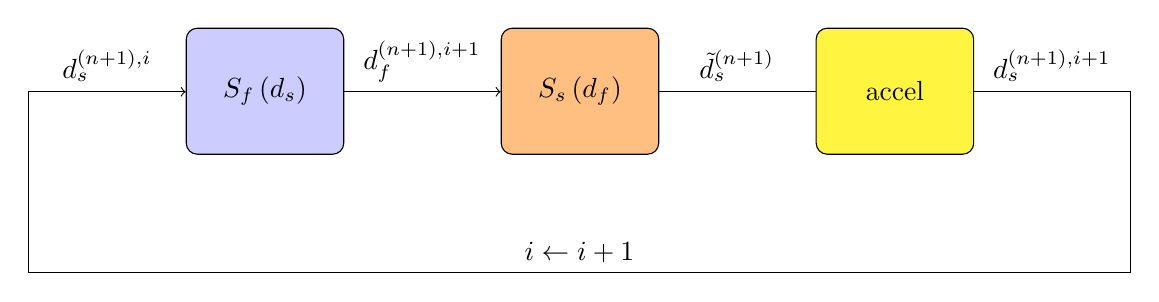
\begin{tikzpicture}[scale=1]
			\tikzstyle{solver}=[draw,rectangle,rounded corners,text centered,inner sep=10pt, anchor=south west, minimum width=2cm,minimum height=1.6cm]
			
			\node[solver,fill=blue!20] at (2,5) {$S_f\left( d_s\right)$};
			\node[solver,fill=orange!50] at (6,5) {$S_s\left(d_f\right)$};
			\node[solver,fill=yellow!75] at (10,5) {accel};
			
			\draw[->] (0,5.8)-- (2,5.8) node[midway,above] {$d_s^{(n+1),i}$};
			\draw[->] (4,5.8)-- (6,5.8) node[midway,above] {$d_f^{(n+1),i+1}$};
			\draw[-] (8,5.8)-- (10,5.8) node[midway,above] {$\tilde{d}_s^{(n+1)}$};
			\draw[-] (12,5.8)-- (14,5.8) node[midway,above] {$d_s^{(n+1),i+1}$};
			
			\draw[-] (14,5.8)-- (14,3.5);
			\draw[-] (0,5.8)-- (0,3.5);
			
			\draw[-] (0,3.5)-- (14,3.5) node[midway,above] {$i \leftarrow i+1$};
			
		\end{tikzpicture}
		\caption{serial implicit coupling}
		\label{fig:serial-implicit}
	\end{subfigure}
	\newline
	\centering
	\begin{subfigure}{.8\textwidth}
		\centering
		% include second image
		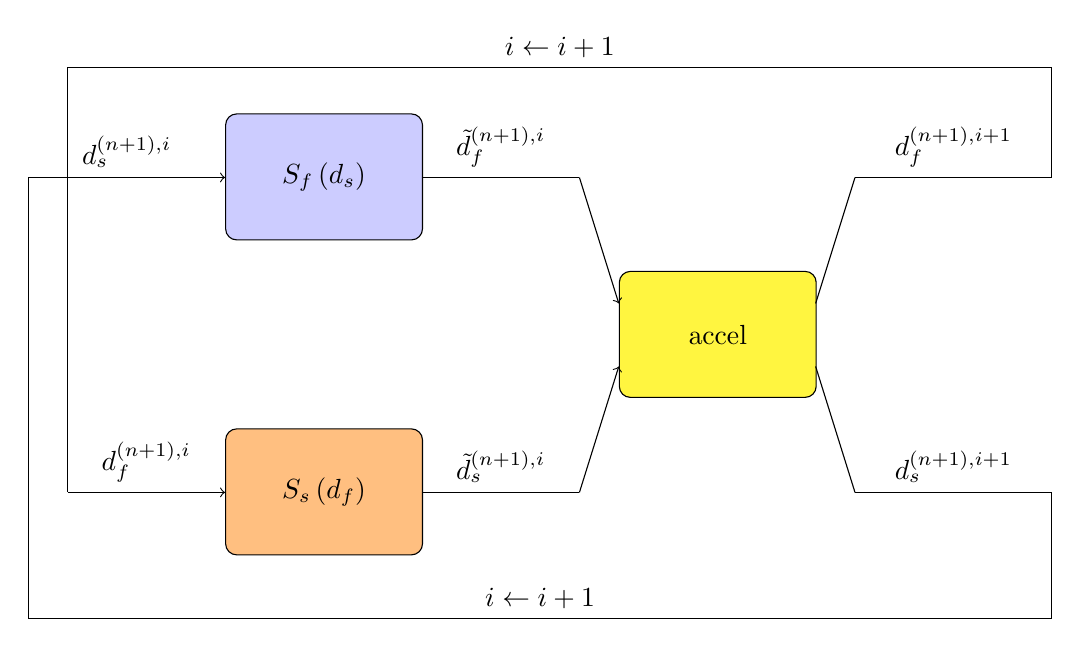
\begin{tikzpicture}[scale=1]
			\tikzstyle{solver}=[draw,rectangle,rounded corners,text centered,inner sep=10pt, anchor=south west, minimum width=2.5cm,minimum height=1.6cm]
			
			\node[solver,fill=blue!20] at (2.5,4) {$S_f\left( d_s \right)$};
			\node[solver,fill=orange!50] at (2.5,0) {$S_s\left(d_f\right)$};
			
			\node[solver,fill=yellow!75] at (7.5,2) {accel};
			
			\draw[->] (0,4.8)-- (2.5,4.8) node[midway,above] {$d_s^{(n+1),i}$};
			\draw[->] (0.5,0.8)-- (2.5,0.8) node[midway,above] {$d_f^{(n+1),i}$};
			
			\draw[-] (5,4.8)-- (7,4.8) node[midway,above] {$\tilde{d}_f^{(n+1),i}$};
			\draw[-] (5,0.8)-- (7,0.8) node[midway,above] {$\tilde{d}_s^{(n+1),i}$};
			
			\draw[->] (7,4.8)-- (7.5,3.2);
			\draw[->] (7,0.8)-- (7.5,2.4);
			
			\draw[-] (10,3.2)-- (10.5,4.8);
			\draw[-] (10,2.4)-- (10.5,0.8);

			\draw[-] (10.5,4.8)-- (13,4.8) node[midway,above] {$d_f^{(n+1),i+1}$};
			\draw[-] (10.5,0.8)-- (13,0.8) node[midway,above] {$d_s^{(n+1),i+1}$};

			\draw[-] (13,4.8)-- (13,6.2);
			\draw[-] (13,0.8)-- (13,-0.8);

			\draw[-] (13,6.2)-- (0.5,6.2) node[midway,above] {$i \leftarrow i+1$};
			\draw[-] (13,-0.8)-- (0,-0.8) node[midway,above] {$i \leftarrow i+1$};
			
			\draw[-] (0,-0.8)-- (0,4.8);
			\draw[-] (0.5,6.2)-- (0.5,0.8);

			%\draw[-] (0,0.8)-- (0,2);
			%\draw[-] (8,0.8)-- (8,2);
			
			%\draw[-] (0,3.6)-- (0,4.8);
			%\draw[-] (8,3.6)-- (8,4.8);
			
			%\draw[-] (8,3.6)-- (0,2) node[midway,above] {$n \rightarrow n+1$};
			%\draw[-] (0,3.6)-- (8,2);
			
			
		\end{tikzpicture}
		\caption{parallel implicit coupling}
		\label{fig:parallel-implicit}
	\end{subfigure}
	\caption{Implicit coupling schemes}
\end{figure}

Implicit methods are generally applicable to any kind of FSI problems, in contrast with explicit methods. When fluid and structure are strongly coupled, explicit coupling can be subject to numerical instabilities, a problem that cannot always be solved by reducing the coupling time step size \cite{van2009added}. These instabilities can be overcome by implicit methods, even if several coupling iterations may be executed every time step, until the values on both sides of the interface converge.


\section{Strong coupling algorithms}
\label{sec:strong-coupling}

As mentioned in the previous chapter, 





\section{Interface Mesh}
\label{sec:interface-mesh}

In this section, FSI methods are classified by means of two different mesh treatment procedures: conforming
or non-conforming techniques. The basic question is, whether fluid and solid mesh need to align
with each other at the FSI interface or not. Unless stated otherwise, the explanations of this section are
taken from [20]. Note that some aspects of conforming mesh methods are already included in the previous
sections without explicitly mentioning so, in order to develop a better understanding of partitioned FSI
simulations.
Conforming mesh methods usually consist of three major subtasks, namely computation in the fluid and
solid domain, as well as interface and mesh movement. They require both fluid and structural meshes
to conform to the wet surface, because the coupling conditions are applied via the interface as physical
boundary conditions for the respective domains. This does not necessarily imply node-to-node matching
of fluid and structure meshes at the interface. This must hold for all time instances, which means that
both fluid and structural grids need to be moved in case deformations of the solid appear. This is a
simple task for the solid mesh, since it is usually expressed in a Lagrangian fashion anyway. However, as
a typical Eulerian fluid mesh would not follow the interface motion, the necessity of the ALE method as
discussed in Section 2.2.3 becomes apparent. Also, mesh smoothing techniques need to be introduced in order to prevent quality losses of the fluid mesh in terms of distorted elements. These irregularities lead
to accuracy loss in simulations. In Figure 3.5, a conforming mesh is shown at two different points in time.
At the first instance (Figure 3.5a) the solid is undeformed and therefore, also the fluid mesh remains in
its initial configuration. In contrast, at the second point in time (Figure 3.5b) the solid is deformed and
the fluid mesh conforms to the displaced wet surface. Consequently, also mesh smoothing is applied.
There is a wide variety of such mesh updating procedures. Some common techniques compute the mesh
movement by considering mesh edges as springs ((torsional) spring analogy), solving the Laplace equation
or solving a pseudo-structural system of equations (see e.g. [18], [43], [20] and their respective references
for further explanations of these techniques). Conforming mesh strategies are widely, but not exclusively
used in partitioned FSI approaches. Furthermore, they typically also utilize the ALE method ([20]).
In contrast, in non-conforming mesh strategies all interface conditions are directly imposed as constraints
on the flow and structural governing equations. Therefore, it is possible to use non-conforming meshes
for fluid and solid domains as they remain geometrically independent from each other. Thus, also mesh
smoothing techniques are obsolete [43]. Figure 3.6 depicts such a situation. By analogy with Figure 3.5,
again the initial configuration (Figure 3.6a) and an instance when the solid is deformed (Figure 3.6b) are
shown. It is clearly visible that the fluid mesh does not conform to the wet surface as all nodes stay at
the same position regardless of the solid deformation.
This approach is mostly used in immersed methods. The considerations in this section are limited to them,
as they are also very common for FSI simulations. Coupling is imposed via additional force-equivalent
terms appearing in the model equations of the fluid, enforcing the kinematic and dynamic conditions.
These FSI forces are computed from the structural model, which is dealt with separately together with
tracking the position of the interface. The forces represent the effects of a boundary or body being
immersed in the fluid domain (leading to immersed boundary and immersed domain methods). A purely
Eulerian mesh can be applied to the whole computational domain for solving the fluid equations, since
the force-equivalent terms are dynamically added in a spatially specific manner to those locations, which
are currently occupied by the structure. After solving the fluid equations, forces exerted on the solid at
the wet surface are computed and used as input for the structural solver, which still employs a Lagrangian
mesh. Subsequently, the deformation of the solid material is calculated and the displacement of the FSI
interface is fed back to the fluid model in form of updated force-equivalent terms ([31], [20], [43]).

\section{Stability: Added Mass Effect}
\label{sec:addedd-mass}

To conclude this chapter about computational aspects of FSI simulations, the AME is briefly described.
Explanations of this effect can be found in a great variety throughout FSI literature, typically explicated
for specific solver strategies or flow regimes (see e.g. [5], [42], [15], [2]). Therefore, in the scope of
this thesis only a short phenomenological introduction to the concept of added mass and numerical
problems arising from it is given. However, this suffices to focus on both weakly and strongly coupled partitioned approaches, which are practically relevant in this thesis. The AME is inherent to partitioned
FSI approaches as the single-physics fields are not continuously coupled but interaction only occurs at a
finite number of discrete time instances, when coupling quantities are exchanged.
As already mentioned in Section 2.3.3, there can be no gaps between structure and fluid. Also their
respective particles cannot occupy the same spatial locations simultaneously. Thus, if the solid is moved,
also fluid particles move. Changing the state of motion of the structural component consequently requires
taking into account inertial effects not only of the solid itself, but also of the surrounding fluid, which
artificially rests for the span of a single structure solver time step. In more descriptive words: Moving the
solid also implies moving fluid particles close to the solid. Therefore, the structure behaves more inert
due to artificially added mass ([42], [2]). Since inertia is dependent on mass and therefore density, the
% AME is also. More precisely, it is dependent on the ratio (MA) of structural (S) und fluid density (F )
([42], [5]):
%MA = S F : (3.1)
This ratio is often used to describe how strong the interaction between solid and fluid is. For cases, in
%which the solid density is much higher than the fluid density (MA  1), this effect does not dominantly
influence the FSI problem (weak interaction). But as fluid and structure densities approach each other
%(MA  1) or the fluid becomes even denser than the solid (MA < 1), its consideration is crucial (strong
interaction) and imposes stability limits on partitioned solution techniques ([5], [42], [2]). Note that the
AME is not only governed by the density ratio of Equation 3.1 but also by geometric properties of the
problem, the stiffness of the solid ([5]) and the speed of sound in the flow domain ([42]). Nonetheless,
for the sake of simplicity and intuitiveness, explanations in this thesis are mostly limited to the density
ratio.
In general, the AME is of bigger concern for incompressible flows than for compressible regimes. From
a physical point of view, deformations of the structural domain can be interpreted as perturbations for
the flow field. In compressible flows the speed of sound (speed at which perturbations propagate through
the flow) is finitely large. Thus, the influence of a geometrical change of the fluid domain caused by
deformations of the solid is locally limited during a certain period of time. In contrast, in incompressible
flows the speed of sound is infinitely large, hence all perturbations propagate through the flow without
time delay. Therefore, regardless of how much time has passed since a perturbation, the whole flow field
is directly affected ([42], [5]).
In the following it is assumed that a weakly coupled algorithm allows computation of the fluid and solid
solution only once per time step. In addition, coupling data is also exchanged once per time instance. In
contrast, a strongly coupled solver does the same at least twice per time increment (for a reminder see
Section 3.2 and compare Figure 3.4). As can be shown, in the compressible case a more dominant AME
can be compensated for by reducing the time step size of strongly coupled, partitioned solution algorithms.
This however, does not hold for the incompressible regime, where even in the limit of vanishing time step
size strongly coupled, partitioned algorithms might fail ([42]). These observations are consistent with the
above mentioned physical explanation.
First of all, considering compressible flows, indeed, the lack of repeated subiterations in weakly coupled
partitioned techniques leads to a strict limit for the density ratio (of Equation 3.1) due to the fact that
the interface conditions are not enforced and energy balance at the wet surface is generally not given.
If that limit is exceeded the algorithm fails due to instability ([2]). Likewise, in such a case a strongly
coupled partitioned algorithm converges slowly, resulting in possibly many necessary subiterations, which
is computationally costly. Yet it does not become unstable, given that the time step size is chosen sufficiently
small. Reducing the time step size to an arbitrarily small extent cannot stabilize a weakly coupled
approach if the stability criterion on the density ratio is not met ([15]). Conversely, the convergence
rate of strongly coupled algorithms increases by the same factor, by which the time step size decreases,
meaning that in the limit of vanishing time step size the monolithic solution is obtained ([5], [42]).
In the incompressible case however, a strict stability limit exists for both weakly and strongly coupled
algorithms. It is independent of the size of time increments1. Furthermore, in order for an implicit
method to achieve the monolithic solution (assuming its convergence is given, i.e. the before mentioned
stability limit is not exceeded) the number of subiterations must be increased as time step size decreases
([15], [42]).
\chapter{Software Packages used in this work}
\label{cha:software}

This chapter illustrates the main software tools used in this work. First, the coupling library \textit{preCICE} is introduced in Section \ref{sec:precice}. Then, the multibody dynamics solver \textit{MBDyn} being connected to preCICE is shortly presented in Section \ref{sec:mbdyn}.


\section{preCICE}
\label{sec:precice}

The main information concerning preCICE is taken from the official documentation: that is \cite{gatzhammer2014efficient} and  \cite{bungartz2016precice}. The preCICE website is also a source of documentation\footnote{\href{http://www.precice.org}{www.precice.org}}.

The open-source\footnote{The code can be accessed via Github: \href{https://github.com/precice/precice}{github.com/precice/precice}} software library preCICE provides the components to connect traditional single-physics solvers and create a partitioned multi-physics simulation (e.g. fluid-structure interaction, conjugated heat transfer, solid-solid interaction, etc.).
It aims at coupling existing solvers in a partitioned black-box manner (see Section \ref{sec:coupling}):  only minimal information abut the solver is available and connection involves just interface nodes. 
In order to be flexible and easily implemented, the impact on the solvers should be as minimal as possible: for this reason, preCICE offers a high level ~\ac{API} (Section \ref{sec:pc-api}) different languages, such as C/C++, Fortran and Python.
The ability to switch among different solvers is advantageous as it provides a lot of flexibility in developing and testing new coupled components.

In a nutshell, preCICE simply affects the input and observes the output of the solvers (called \textit{participants}). The required data and control elements are accessed using an \textit{adapter}, i.e. a "glue code" that is attached to the corresponding solver and communicates the information with the library.

preCICE performs all the actions required to perform a coupled simulation: implements the coupling strategy and convergence criteria (Section \ref{sec:pc-coupling}), the communication
between the participants (Section \ref{sec:pc-comm}), the mapping of data between meshes (Section \ref{sec:pc-map}). preCICE is configured by means of an ~\ac{XML} file (Section \ref{sec:pc-config}).



\subsection{Implemented coupling strategies}
\label{sec:pc-coupling}

The \textit{partitioned approach} (Section \ref{sec:coupling}) is obviously the coupling strategy adopted by preCICE. It allows both \textit{explicit} (Section \ref{subsec:explicit}) and \textit{implicit} coupling (Section \ref{subsec:implicit}). The possible variants are four:

\begin{itemize}
	\item \texttt{serial-explicit}: a serial, weakly coupled algorithm (Figure \ref{fig:serial-explicit}). The first solver uses the second solver solution at the last time step to compute its current solution. In contrast, the second solver needs the current first solution to compute its solution at the same time instance. The order of execution is user defined.
	\item \texttt{parallel-explicit}: both solvers advance in parallel (Figure \ref{fig:parallel-explicit}) and exchange data at the end of each time step, resulting in a less stable procedure. The bottleneck of this procedure is related to the most time consuming solver.
	\item \texttt{serial-implicit}: a serial strongly coupled algorithm (Figure \ref{fig:serial-implicit}). The user can define the order of execution, the coupling algorithm (basically all the algorithms described in Section \ref{sec:strong-coupling}) and its parameters in a section of the configuration file named \texttt{acceleration}.
	\item \texttt{parallel-implicit}: again both solvers execute in parallel (Figure \ref{fig:parallel-implicit}). An implicit scheme modifies the result of the fixed-point iteration on both data \cite{mehl2016parallel}. 
\end{itemize}



\subsection{Communication strategies}
\label{sec:pc-comm}

All the participants need to communicate with each other, in order to share coupling data.
Each solver might be executed in multiple processes or on different nodes of a cluster (\textit{intrafield parallelism}).
This form of parallelization requires efficient forms of communication between the solver in order to avoid that data transfer becomes a bottleneck during a simulation.

preCICE implements a fully parallel process-to-process communication approach \cite{Shukaev2015} using:

\begin{itemize}
	\item \textit{~\ac{MPI}}: available on 	most scientific computers, it may be necessary to adapt/change the MPI versions of the respective single-physics solvers or of preCICE.
	\item \textit{~\ac{TCP/IP}}: popular means of network communication and free of incompatibilities between versions.
\end{itemize}

As to performances, MPI is the best technique especially when a high numbers of nodes is present. Anyway, socket communication is quite as fast, such that
both techniques are very well-suited for larger-scale simulations \cite{gatzhammer2014efficient}.

In each solver, executed in parallel, one "master" process is defined to manage the progress of the simulation. No central node is required. The participating
processes use asynchronous point-to-point (M:N) communication. The channels are static and defined in the beginning of the simulation. This sets a limit in using preCICE with dynamically adaptive meshes or immersed boundaries.

\subsection{Data mapping}
\label{sec:pc-map}

Even if volume coupling is possible, preCICE is mainly designed to couple simulations that share a common surface boundary (namely \textit{conforming meshes}, in the terminology used in Section \ref{sec:conforming-mesh}). The meshes don't need to be node-to-node coincident, so it is necessary to map variables at the interface, preserving the geometry (i.e. no gaps or superpositions at the interface) and the mass and energy balances. 

The user defines which data are shared by each \textit{participant} (i.e. solver) and the way data is shared in the configuration section named \texttt{mapping}. As described in Section \ref{sec:data-mapping}, two kinds of mapping are available:

\begin{itemize}
	\item \texttt{consistent}: the value of a node at the one grid is the same as the value of the corresponding node (or nodes) at the other grid. In general the number of fluid nodes is at least the same or, more often, exceeds the nodes of the structure, so a single structural node is associated to several fluid nodes. The mapping of displacements is consistent: in the simplest case, all fluid nodes experience the same displacement of a single solid node, otherwise an interpolation is performed (see Figure \ref{fig:consistent}).
	\item \texttt{conservative}: in the same conditions as before, forces are mapped from multiple fluid nodes to a single solid node in an additive manner (see Figure \ref{fig:conservative}).
\end{itemize} 

Along with the mapping strategy, a method must be defined (see Section \ref{sec:data-mapping}): \texttt{nearest-neighbor}, \texttt{nearest-projection}, \texttt{rbf}. For the latest method, preCICE implements a wide variety of basis functions, with Gaussian and thin plate splines being the most widely used.

 

\subsection{Configuration}
\label{sec:pc-config}

In order to run a multi-physics simulation with preCICE, all the participating, \textit{adapted} solvers have to be started (the order is irrelevant).
Some configuration files are needed:

\begin{itemize}
	\item each adapter in general needs its own configuration file. It normally contains information about the boundaries (wet-surface) used for the coupling, names of exchanged data, mesh and the name of the common preCICE configuration file, plus other parameters, specific to the adapter. The one for the MBDyn adapter will be described in more detail in Chapter \ref{cha:adapter} and in Appendix \ref{app:mbd-config-file}.
	\item preCICE configuration file: This is an XML file and each participant points at it. It defines all the information relevant to the simulation:
	\begin{itemize}
		\item type and name of exchanged data and meshes over which those data are passed
		\item which solvers participate in the simulation, which data produce or consume, and how the mapping is performed
		\item how solvers communicate among each other
		\item coupling scheme and all the necessary information 
	\end{itemize}
	
	The structure of a preCICE configuration file is illustrated in Appendix \ref{app:pc-config-file}.
		
\end{itemize}


\subsection{Application Program Interface}
\label{sec:pc-api}

A solver, in order to be coupled to preCICE, must either provide a way to access its core functions (e.g. initialize, set input data, read output, advance...) from outside the code (via API, socket, etc...) or it has to be slightly modified in order to perform all the operations required by the preCICE library.

The result is an \textit{adapter}, which can be the modified and recompiled original solver, or a standalone piece of code that communicates with the original unmodified solver on one side and with the preCICE library on the other. The adapter groups together all the calls to the preCICE methods from its API (a list of the API calls, taken from the official documentation, can be found in Appendix \ref{sec:api-code}).

While preCICE is written in C++, there exist APIs also for other languages, so that the adapter can be written also in C, Fortran or Python.

A coupling consists of a configuration and an initialization phase, multiple coupling advancements and a finalization phase: the general structure of an adapter can be found in \ref{sec:adapter-code}.


\subsection{Official Adapters}
\label{sec:pc-adapters}


This work introduces an adapter to preCICE for MBDyn. It is based on previous MBDyn adapters and on the examples given on the preCICE website\footnote{\href{https://github.com/precice/precice/wiki/Adapter-Example}{github.com/precice/precice/wiki/Adapter-Example}}.
Official adapters are currently available for several free solvers, e.g. CalculiX, Code-Aster and SU2. Also some closed-source software packages are supported. A (maybe outdated) list of official adapters can be found in \cite{uekermann2017official}, while the current status of coupled codes can be found at the following link: \href{https://www.precice.org/codes/}{preCICE adapters}.


\section{MBDyn}
\label{sec:mbdyn}


MBDyn is free and open-source\footnote{the software is available through a public git repository \href{https://gitlab.polimi.it/Pub/mbdyn}{gitlab.polimi.it/Pub/mbdyn}} general purpose Multibody Dynamics analysis software developed at the \textit{Dipartimento di Scienze e Tecnologie Aerospaziali}  of the University Politecnico di Milano.

Most of the information concerning MBDyn is taken from the official documentation given in the software website\footnote{MBDyn website: \href{https://www.mbdyn.org/}{mbdyn.org}} and form the input manual\footnote{a copy can be found at the following link [\href{https://www.mbdyn.org/userfiles/documents/mbdyn-input-1.7.3.pdf}{input manual}] or in the code repository}.

MBDyn allows to build a simulate multibody system, which\footnote{see Wikipedia entry: \href{https://en.wikipedia.org/wiki/Multibody_system}{Multibody system}} is the study of the dynamic behavior of interconnected rigid or flexible bodies, each of which may undergo large translational and rotational displacements.

MBDyn can simulate linear and non-linear dynamic or rigid and flexible bodies (including geometrically exact and composite-ready beam and shell finite elements, component mode synthesis elements, lumped elements) subjected to kinematic constraints, external forces and control subsystems\cite{masarati2014efficient}. 
MBDyn has been developed to serve as an analysis tool for rotorcraft research and cab simulate essential fixed-wing and rotorcraft aerodynamics.

As explained more in detail later, MBDyn is open to be connected to other software components to perform multiphysics simulations. In particular, it is possible to pass externally computed forces  and to steer the multibody simulation from an external API: this feature has been particularly useful in building and \textit{adapter} to couple MBDyn with the library preCICE (see Chapter \ref{cha:adapter}).

In this section we give a short introduction to some of the relevant features of MBDyn, starting form basic information on the input file syntax (Section \ref{sec:mbd-syntax}), and the output files (Section \ref{sec:mbd-output}). Then some of the elements relevant for the description of the models used in the this work are presented: nodes (Section \ref{sec:mbd-node}), beam elements (Section \ref{sec:mbd-beam}), bodies (Section \ref{sec:mbd-body}) and forces (Section \ref{sec:mbd-forces}). 


\subsection{Basic syntax}
\label{sec:mbd-syntax}

MBDyn is a command line tool and can be generally started from a terminal passing an input file containing all the information required to perform a simulation. 

The input files is structured in blocks and each block has a syntax described in Backus Naur form in the input manual.

\lstset{language=mbdyn}
\begin{lstlisting}[caption=MBDyn input file structure,label=lst:mbd-struct]
begin : data ;
    # select a problem
    problem : initial value ;
end : data ;

begin : initial value ;
    # problem-specific data
end : initial value ;

begin : control data ;
    # model control data
end : control data ;

begin : nodes ;
    # nodes data
end : nodes ;

begin : elements ;
    # elements data
end : elements ;
\end{lstlisting}

As illustrated in listing \ref{lst:mbd-struct}, statements are logically divided in blocks. Each block is opened by a \texttt{begin} statement and it is closed by an \texttt{end} statement.

The sequence of relevant valid blocks is:

\begin{itemize}
    \item \texttt{data}: defines the kind of problem to be solved by the analysis. The most significant one is \texttt{initial value} and is already defined in the example. 
    \item type of problem:  block takes the name of the problem defined in the data block (\texttt{initial value} in this case) and contains all the information required by the integration method to perform the desired simulation (e.g. simulation type, time step, number of iterations, tolerance ...).
    \item \texttt{control data}: mostly contains information about the problem that is required to ensure that a consistent model will be generated (i.e. the number of nodes, elements, forces...).
    \item \texttt{nodes}: The nodes block contains all the nodes required by the simulation. They are are defined as the entities that make degrees of freedom available to the simulation, so they must exist before any element is generated.
    \item \texttt{elements}: contains all the elements. They are defined as the entities that generate equations using the degrees of freedom provided by the nodes.
\end{itemize}

We focus now on the main entities of a MBDyn simulation, namely nodes and elements. A detailed example of the input file used in most simulations in this work can be found in Appendix \ref{sec:mbdyn-input-file}.


\subsection{Nodes}
\label{sec:mbd-node}

Nodes are the basic blocks of a model: they instantiate kinematic degrees of freedom and the corresponding equilibrium equations. There can be different type of nodes in MBDyn, we focus here on \texttt{structural nodes}.

Structural nodes can have 3 degrees of freedom, thus describe the kinematics of point mass motion in space  (position) or 6 DoFs (position and orientation), and thus describe the kinematics of rigid-body motion in space.

Each node has a unique label and can be specified in different ways:

\begin{itemize}
	\item \texttt{static}: this keyword instantiates only equilibrium equations (force for 3 DoF nodes or force and moment for 6 DoF nodes)
	\item \texttt{dynamic}: this also instantiates momentum (3 and 6 DoFs) and momenta moment (6 DoFs)
\end{itemize}

Also \texttt{modal} and \texttt{dummy} nodes exist, but are beyond the scope of this work.

Nodes are the starting point to define the elements of a simulation.


\subsection{Elements}
\label{sec:mbd-elem}

Elements constitute the components of the multibody model. Each has a unique numerical label and is connected to one or more nodes. They write contributions to nodes equations and represent \textit{connectivity} and \textit{constitutive properties}.

%Elements that require both displacement and orientation can only be connected to 6 DoFS nodes.

There exist many types of elements in MBDyn, we focus here on the ones used in the FSI simulation: beams, bodies, joints and forces.



\subsection{Beam elements}
\label{sec:mbd-beam}

As briefly introduced in Section \ref{sec:beam}, when simulations involve slender bodies, it is particularly interesting to use a 1D finite element model together with a form of mapping between the interface (wet surface) and the model to exchange kinematics and dynamics information. This can be performed in MBDyn using \texttt{beam} elements (described in this section) and the \texttt{external structural mapping} element (described in Section \ref{sec:mbd-forces}).

MBDyn models slender deformable components by means of finite volume \texttt{beam} elements with a high level of flexibility.

The beam element is defined by its nodes and a reference line; although 2 and 3 nodes beam elements are implemented, only \texttt{beam3} are considered here (Figure \ref{fig:mbdyn-beam-model}). Each node of the beam is related to a \texttt{structural node} (node 1 to 3 in Figure \ref{fig:mbdyn-beam-model}) by an offset ($o_1$ to $o_3$) and a relative orientation.

\begin{figure}[htbp!]
	\centering
	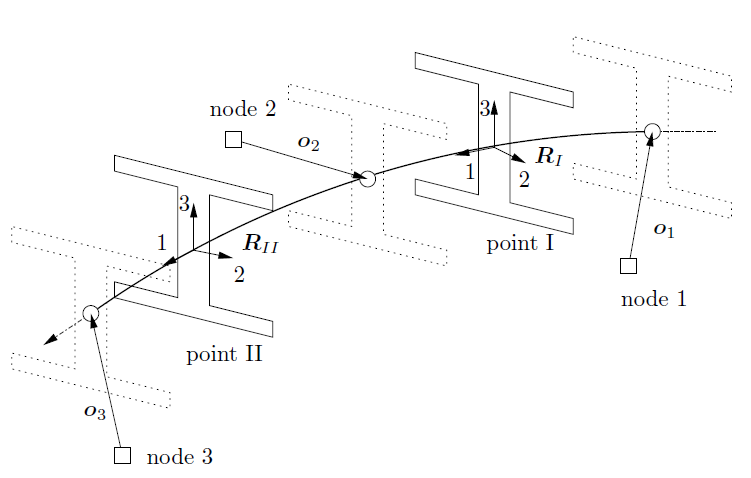
\includegraphics[width=0.8\textwidth]{images/beam_model}
	\caption{MBDyn beam model, taken from the input manual}
	\label{fig:mbdyn-beam-model}
\end{figure}


The Finite Volume approach described \cite{ghiringhelli2000multibody} is used to model the beam element. It computes the internal forces as functions of the reference line strain and as functions of the  orientation at the \textit{evaluation points} (i.e. integration points, point I and II in Figure \ref{fig:mbdyn-beam-model}) that are between nodes 1 and 2, and between nodes 2 and 3 (at $\xi =-1/\sqrt{3}$ and $\xi = 1/\sqrt{3}$ of a non-dimensional abscissa $-1\leq \xi \leq 1$ ranging from node 1 to node 3).


A 6D constitutive law is defined at each evaluation point: it relates the strains and the curvatures of the beam (and their time derivatives) to the internal forces and moments at the evaluation points in the form:

\begin{equation}
	\begin{Bmatrix}
		F_x \\ F_y \\ F_z \\ M_x \\ M_y \\ M_z
	\end{Bmatrix} = f
	\begin{pmatrix}
		\begin{Bmatrix}
			\epsilon_x \\ \gamma_y \\ \gamma_z \\ \kappa_x \\ \kappa_y \\ \kappa_z
		\end{Bmatrix} , 
		\begin{Bmatrix}
			\dot{\epsilon_x} \\ \dot{\gamma_y} \\ \dot{\gamma_z} \\ \dot{\kappa_x} \\ \dot{\kappa_y} \\ \dot{\kappa_z}
		\end{Bmatrix}
	\end{pmatrix}
\end{equation}


Using the convention of \textit{x-axis} as beam axis we have:

\begin{itemize}
	\item $F_x$: axial force component,
	\item $F_y$ and $F_z$: shear force components,
	\item $M_x$: torsional moment component,
	\item $M_y$ and $M_z$: bending moment components,
	\item $\epsilon_x$: axial strain component,
	\item $\gamma_y$ and $\gamma_z$: shear strain components,
	\item $\kappa_x$: torsional curvature component,
	\item $\kappa_y$ and $\kappa_z$: bending curvature components,
	\item $f$: constitutive law.
\end{itemize}


\subsubsection{Beam section Constitutive Law}

In dynamic simulations, linear elastic or viscoelastic laws are generally used, even though nonlinear laws can be used.  Focusing on linear laws, MBDyn allows the user to define every constitutive laws, going from an isotropic beam section to a fully anisotropic one: in fact the entire $6 \times 6$ constitutive matrix can be provided. It is up to the user to define a valid law as the matrix must satisfy some constraints, e.g. it must be symmetric.

In the context of FSI simulations, this feature allows the user to define a section constitutive law that is independent from the shape of the beam itself. Thus the aerodynamic aspects and the structural aspects are handled by two distinct elements of the model: i.e. the interface mesh defines the aerodynamic forces and the beam constitutive law defines the structural properties.   

Some studies about the definition of general beam section constitutive properties (\textit{composite beam section characterization}) are available in the literature: an early work can be found in \cite{giavotto1983anisotropic}, a review in \cite{hodges1990review} or an application to wind turbine blades in \cite{kim2013development}.


\subsection{Bodies}
\label{sec:mbd-body}

The \texttt{body} element describes a lumped rigid body when connected to a regular, 6 DoF structural node, or a point mass when connected to a rotationless, 3 DoF structural node. It can be used in connection with a structural element to give inertial properties: for example, in a \texttt{beam} element (see Section \ref{sec:mbd-beam}), 2 bodies are added to the evaluation points of the beam to account for lumped inertia of each portion in which the beam is divided. 


\subsection{Joints}
\label{sec:mbd-joint}

\texttt{structural} nodes can be constrained by means of \texttt{joint} elements. Many different joints are available. In the FSI model the following types of joints are used:

\begin{itemize}
	\item \texttt{clamp}: grounds all 6 DoFs of a node in an arbitrary position and orientation
	\item \texttt{total joint}: allows to arbitrarily constrain specific components of the relative position and orientation of two nodes\cite{masarati2013formulation}
\end{itemize}


\subsection{Forces}
\label{sec:mbd-forces}

The \texttt{force} element is a general means to introduce a right-hand side to the equations. Structural forces are specific to structural
nodes and  have three components that may depend on arbitrary parameters and a location in space.

MBDyn allows to communicate with an external software that computes forces based on information on the kinematics of the model. This feature is at the basis of the development of the \textit{adapter}. The following elements can be used.


\subsubsection{External Structural}

The \texttt{External Structural} element allows to communicate with an external software that computes forces applied to a pool of \texttt{nodes} and may depend on the kinematics of those nodes. In this case forces are applied directly to the nodes. In a FSI model, this would require that each interface mesh node has a correspondent MBDyn structural node. 

\subsubsection{External structural mapping}

This element is similar to the previous one, but the nodes where forces are applied and the kinematics is computed depend on structural nodes through a linear mapping. This element has been used in building the adapter. In order to use the \texttt{external structural mapping} elements, the following steps have to be performed:

\begin{enumerate}
	\item a set of points is defined for each \texttt{structural node} according to a specified offset. Those points are used to compute the kinematics of the interface points, originating from the rigid-body motion of the structural nodes
	\item before the simulation, a linear mapping matrix $H$ is generated starting from the position of the above points and the interface mesh points (this is performed by means of an \texttt{Octave} script which is part of MBDyn). The matrix is stored in sparse form
	\item the mapping matrix is used during simulation to map forces and kinematics between the interface nodes and the structural nodes
\end{enumerate}

The constant matrix mapping allows to compute the position and the velocity of the \textit{interface} points as function of the points rigidly offset from structural nodes:

\begin{subequations}
	\begin{eqnarray}
		x_{interf} &=& H x_{mbdyn} \\
		\dot{x}_{interf} &=& H \dot{x}_{mbdyn} 
	\end{eqnarray}
\end{subequations}

The same matrix is used to map back the forces onto structural nodes based on the preservation of the work done in the two domains:

\begin{equation}
	\delta x_{mbdyn}^T \cdot f_{mbdyn} =  \delta x_{interf}^T \cdot f_{interf} = \delta x_{mbdyn}^T \cdot H^T \cdot f_{interf} 
\end{equation}

which implies

\begin{equation}
	f_{mbdyn} = H^T f_{interf}
\end{equation}

When performing an FSI simulation with strong coupling (see Section \ref{sec:strong-coupling}), MBDyn may need to compute multiple iterations of the same time step in order to reach global convergence. This is performed by using the keyword \texttt{tight} in the coupling of the \texttt{external structural mapping}. The computation and the communication pattern is the following:

\begin{enumerate}
	\item MBDyn sends the predicted kinematics for time step $k$
	\item MBDyn receives a set of forces sent by the external peer; those forces are computed based on the kinematics at iteration $j$
	\item MBDyn continues iterating until convergence using the last set of forces until, while reading the forces, it is informed that the external peer converged. this implies that MBDyn solves the kinematics for time step $k$ at iteration $j$ using the forces evaluated by the external solver for iteration $j-1$ 
\end{enumerate}

The communication with the external software, in our case the adapter itself, is performed by means of a local unix socket.


\subsection{Simulation output}
\label{sec:mbd-output}

There are a bunch of output files regarding a simulation performed with MBDyn. the name of those files is specified with the option \texttt{-o} (otherwise the name is the same as the input file) and the extensions are:

\begin{itemize}
    \item \texttt{.out}: for miscellaneous output
    \item \texttt{.mov}: for kinematic output of the nodes
    \item \texttt{.ine}: for the dynamic output of the nodes
    \item \texttt{.frc}: for the output of force elements
    \item \texttt{.act}: for the output of beam elements
    \item \texttt{.jnt}: for the output of joint elements
\end{itemize}

The \texttt{.out} file contains information regarding the simulation iterations residuals while other files are described in more detail in Appendix \ref{sec:mbdyn-output-file}.



%
%output
%
%If we copy the above written code to a file called, say, “rigidbody”, and invoke
%mbdyn -f rigidbody
%after a while we obtain the results of the simulation in a set of files called “rigidbody.<ext>”.
%In this case, the extensions will be:
%• out for miscellaneous output
%• mov for the kinematic output of the node
%• ine for the dynamic output of the node
%• frc for the output of the force
%The first file (out) will be ignored at present. The second file (mov) will contain Nnodes
%by Ntimesteps lines formatted as:
%• the node label
%• the three coordinates of the position of the node
%• the three Euler-like angles that define the orientation of the node (following the
%1, 2, 3 convention)
%• the three components of the velocity of the node
%• the three components of the angular velocity of the node
%all the above mentioned quantities are expressed in the global inertial frame
%




\chapter{MBDyn Adapter and its integration}
\label{cha:adapter}
Lorem ipsum dolor sit amet, consectetur adipisci elit, sed eiusmod tempor incidunt ut labore et dolore magna aliqua. Ut enim ad minim veniam, quis nostrum exercitationem ullam corporis suscipit laboriosam, nisi ut aliquid ex ea commodi consequatur. Quis aute iure reprehenderit in voluptate velit esse cillum dolore eu fugiat nulla pariatur.
\chapter{Validation Test Cases}
\label{cha:tests}


\section{Introduction}

In order to validate the coupling adapter developed in this work, a set of test cases have been simulated, which are supposed to qualitatively and quantitatively confirm the physically correctness of the implementation.

The validation has been carried out in different steps: the first task (section \ref{sec:dummy}) consisted in validating the MBDyn model that has been used throughout the simulations and verifying that the implementation of the coupling works as expected.

The second step aimed at comparing the results obtained performing an FSI simulation with MBDyn with another structural solver, both in compressible and in incompressible regime (Sections \ref{sec:cx-mbd} and \ref{sec:su2-mbd}).

Then, some results obtained from FSI simulations coupling MBDyn with OpenFOAM, have been compared with some benchmarks present in literature. At first, the problem described in \cite{ramm1998fluid} has been considered (see Section \ref{sec:sq-cyl-bench}): it is composed of a square bluff body with a trailing flap. It is characterized by a mass ratio (see Section \ref{subsec:mass-ratio}) of $1.18\cdot 10^{-3}$, this turned out to be a fundamental parameter fo the convergence of simulations, and has been extensively analyzed in the subsequent sections.

One set of well-known benchmarks in FSI literature are the three Turek-Hron FSI test cases described in \cite{turek2006proposal}. Those cases are characterized by the same domain (a round cylinder with a trailing flap) and the same fluid properties. Changes impact only fluid velocity and structural properties (in particular $\rho,E$).

At first, the so-called FSI2 benchmark (characterized by a mass number of $0.1$) has been considered (Section \ref{sec:FSI2}). This benchmark, together with the previous one, shows the validity of the adapter and its potential use in FSI simulations.

Finally, the FSI3 benchmark has been extensively analyzed (Section \ref{sec:FSI1-FSI3}). It has a mass number of $1$ and, up to now, it hasn't been possible to find a suitable set of coupling parameters that can make this case converge when coupled with MBDyn.

It appears that the added mass effect (see Section \ref{sec:added-mass}), plays a dominant role in the convergence of a FSI problems with MBDyn. For this reason, a sensitivity analysis has been performed on the FSI3 problem setup (Section \ref{sec:FSI3-sensitivity}). In particular, flow velocity, fluid density and solid stiffness have been varied in order to gain some insight about the range of parameters, and adimensional numbers that must be considered to understand how critical a simulation can be.     

Each section starts with a short description of the test case, including the most relevant parameter: e.g. the fluid domain geometry and discretization, structural and coupling parameters. Finally some results are presented, together with the coupling performances.

The meshes for all test cases have generated with the free software \textit{Salome}\footnote{\href{https://www.salome-platform.org/}{salome-platform.org/}}. Files for MBDyn interface points have been generated by a Python script running within the \textit{Salome} environment. The script is part of the software made for this work. 


\section{Dummy fluid solver}
\label{sec:dummy}

The first task implemented to validate the adapter consisted in developing a simple \textit{dummy fluid solver}: i.e. a software component connected to the coupling library preCICE with the simple task to apply forces to user-defined nodes on the structure and read back the displacements of the interface nodes.

This approach allowed first to validate the MBDyn model with the \texttt{external structural mapping} component (see Section \ref{sec:mbd-forces}) and the correct data exchange between preCICE and the adapter. 

The \textit{dummy solver} has been written in Python and it is part of the software package in this work.

A MBDyn cantilever beam model composed of 5 \texttt{beam3} elements (see Section \ref{sec:mbd-beam}) has been written to perform this test, as depicted in Figure \ref{fig:cnt-beams}. This requires a total of 11 \texttt{node} elements to define the structure.

The beam section is uniform and rectangular ($w \times h$) and the physical properties (eg. $\rho, E, \nu$) are constant throughout the beam length. 

\begin{figure}[htbp!]
	    \centering
        \begin{tikzpicture}
            \point{a}{0}{0};
            \point{b}{1.5}{0};
            \point{c}{3}{0};
            \point{d}{4.5}{0};
            \point{e}{6}{0};
            \point{f}{7.5}{0};
            
            \beam{4}{a}{b};
            \beam{4}{b}{c};
            \beam{4}{c}{d};
            \beam{4}{d}{e};
            \beam{4}{e}{f};
            
            \notation{2}{b}{};
            \notation{2}{c}{};
            \notation{2}{d}{};
            \notation{2}{e}{};
            \notation{2}{f}{};
            
            \notation{4}{a}{b}[ $1$ ];
            \notation{4}{b}{c}[ $2$ ];
            \notation{4}{c}{d}[ $3$ ];
            \notation{4}{d}{e}[ $4$ ];
            \notation{4}{e}{f}[ $5$ ];
            
            \support{3}{a}[-90];
            % \load{1}{b}[90][1][.1];
            
            \dimensioning{1}{a}{f}{-1.8}[$L$];
            \dimensioning{1}{a}{b}{-1}[$l$];
            
            \dscaling{3}{0.5};
            \daxis{1}{-1.5 ,0 ,0}[right][above][left];
        \end{tikzpicture}
    	\caption{cantilever made of 5 beam elements}
		\label{fig:cnt-beams}
\end{figure}

The inertia of the structure is provided by 2 \texttt{body} elements (see Section \ref{sec:mbd-body} attached to the second and third nodes of each beam (see Figure \ref{fig:mbdyn-beam-model}). The center of gravity of each body is offset by $-l/4$ in x-direction (where $l$ is the length of the single beam element). Each body has the following inertial properties (see Figure \ref{fig:cnt-mass}): 

\begin{equation}
    m = \rho wh \frac{l}{4} \quad I = \frac{m}{12} \begin{bmatrix} h^2+w^2 & 0 & 0 \\ 0 & \frac{l^2}{16} + w^2 & 0 \\ 0 & 0 & \frac{l^2}{16} + h^2 \end{bmatrix}
    \label{eq:body-inertia}
\end{equation}


\begin{figure}[htbp!]
	    \centering
\begin{tikzpicture}[every edge quotes/.append style={auto, text=blue}]
  \pgfmathsetmacro{\cubex}{4}
  \pgfmathsetmacro{\cubey}{2}
  \pgfmathsetmacro{\cubez}{3}
  \draw [draw=blue, every edge/.append style={draw=blue, densely dashed, opacity=.5}, fill=yellow!10]
    (0,0,0) coordinate (o) -- ++(-\cubex,0,0) coordinate (a) -- ++(0,-\cubey,0) coordinate (b) edge coordinate [pos=1] (g) ++(0,0,-\cubez)  -- ++(\cubex,0,0) coordinate (c) -- cycle
    (o) -- ++(0,0,-\cubez) coordinate (d) -- ++(0,-\cubey,0) coordinate (e) edge (g) -- (c) -- cycle
    (o) -- (a) -- ++(0,0,-\cubez) coordinate (f) edge (g) -- (d) -- cycle;
  \path [every edge/.append style={draw=black, |-|}]
    (b) +(0,-5pt) coordinate (b1) edge ["$l/2$"] (b1 -| c)
    (b) +(-5pt,0) coordinate (b2) edge ["h"] (b2 |- a)
    (c) +(3.5pt,-3.5pt) coordinate (c2) edge ["w"] ([xshift=3.5pt,yshift=-3.5pt]e)
    ;
    \daxis{1} {-8,-1,-1.5} [right][above][left];
    \dpoint{q}{-2.5}{-1}{-1.5};
    \dpoint{r}{0}{-1}{-1.5};
    \dpoint{s}{-\cubex}{-1}{-1.5};
    \dpoint{t}{\cubex}{-1}{-1.5};
    \beam{4}{q}{r};
    \dhinge{1}{q};
    \dhinge{1}{r};
    \dhinge{1}{s};
    \dhinge{1}{t};
    \dnotation{1}{q}{CoG};
    \dnotation{1}{r}{$n_2$};
    \dnotation{1}{s}{$n_1$};
    \dnotation{1}{t}{$n_3$};
    \ddimensioning{xy}{q}{r}{1.5}[ $l/4$ ];
    \ddimensioning{xy}{s}{t}{-2.5}[ $l$ ];
    
\end{tikzpicture}
    	\caption{\texttt{body} element attached to node 2 of the \texttt{beam} element}
		\label{fig:cnt-mass}
\end{figure}


The first node of the structure is clamped (to implement the cantilever constraint), while all other joints are constrained to move in the $x-y$ plane and rotate only around the $x-axis$ so that the structure can move only in the $x-y$ plane.
The interface mesh is represented in Figure \ref{fig:mbdyn-mesh}. Only the connectivity elements belonging to the $x-z$ and $y-z$ plane are represented, but it does not affect the behavior if the structure.


\begin{figure}[htbp!]
	\centering
	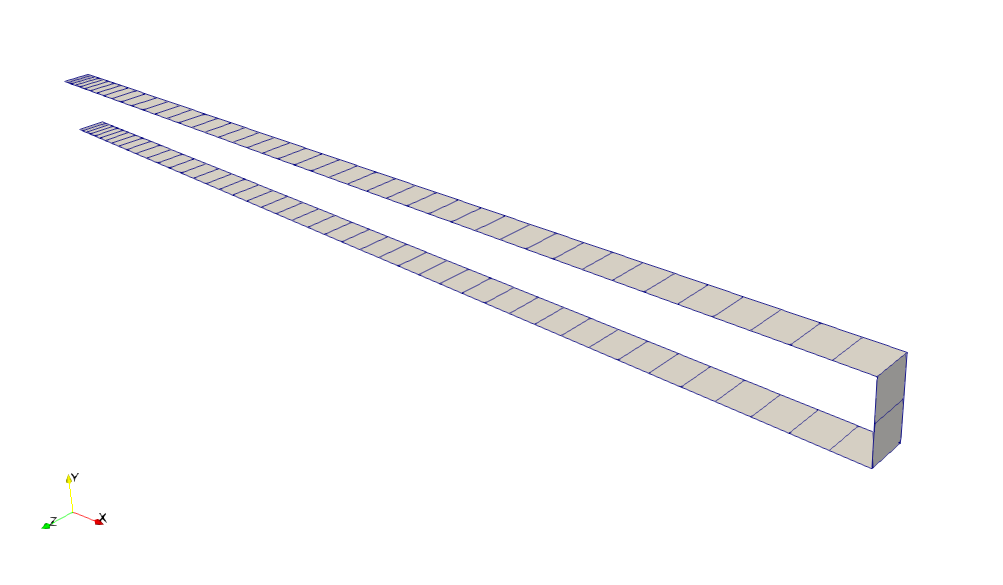
\includegraphics[width=0.7\textwidth]{images/example-mesh}
	\caption{interface points mesh}
	\label{fig:mbdyn-mesh}
\end{figure}

The model has been loaded by a concentrated load on two tip nodes (Figure \ref{fig:cnt-tip}) and with an equivalent distributed load on the nodes belonging to the upper surface (Figure \ref{fig:cnt-distrib}).

\begin{figure}[htbp!]
	%\centering
	    \begin{subfigure}{.8\textwidth}
	    \centering
        \begin{tikzpicture}
            \point{a}{0}{0};
            \point{b}{6}{0};
            \beam{4}{a}{b};
            \support{3}{a}[-90]
            \load{1}{b}[90][1][.1];
        \end{tikzpicture}
    	\caption{cantilever with tip load}
		\label{fig:cnt-tip}
	    \end{subfigure}
	    %\newline
	    \par\bigskip
	    \begin{subfigure}{.8\textwidth}
		\centering
		\begin{tikzpicture}
            \point{a}{0}{0};
            \point{b}{6}{0};
            \beam{4}{a}{b};
            \support{3}{a}[-90]
            \lineload{1}{a}{b}[1][1];%[force interval];
        \end{tikzpicture}
    	\caption{cantilever with distributed load}
		\label{fig:cnt-distrib}
	    \end{subfigure}
	\caption{model and data exchange test-cases}
\end{figure}

The results have been compared the expected theoretical values in terms of tip displacement at steady state and in terms of frequency of the tip movement when the system has been loaded with a step load.

When both the MBDyn model and the data exchanged through the preCICE interface have been validated, the model has been coupled to a CFD solver.





\section{Vertical flap: incompressible regime}
\label{sec:cx-mbd}

The first validation step consisted in comparing the results obtained with MBDyn with the ones given by another structural solver with the same fluid model. 

For this purpose a simple case of a vertical flap immersed in a flow in incompressible regime, has been considered, borrowing an example given in the preCICE website.

\subsection{Fluid domain}

The fluid domain is represented in Figure \ref{fig:ex1-domain}. The inlet is on the left with uniform flow velocity, the outlet is on the right, while all other boundaries are \textit{no-slip} walls.


\begin{figure}[htbp!]
	\centering
	\begin{tikzpicture}
	    \pgfmathsetmacro{\xa}{-0.1}
	    \pgfmathsetmacro{\xb}{0.1}
		\point{a}{-4}{0};
		\point{b}{\xa}{0};
		\point{c}{\xb}{0};
		\point{d}{8}{0};
		\point{e}{\xa}{1};
		\point{f}{\xb}{1};
		\point{g}{-4}{3};
		\point{h}{8}{3};
		
		\point{i}{-3.5}{0.5};
		
		\beam{2}{a}{b};
		\beam{2}{c}{d};
		\beam{2}{a}{g};
		\beam{2}{d}{h};
		\beam{2}{g}{h};
		\beam{4}{b}{e};
		\beam{4}{e}{f};
		\beam{4}{f}{c};
		
		\dimensioning{1}{g}{h}{3.5}[$20m$];
		\dimensioning{1}{a}{b}{-0.6}[$4m$];
		\dimensioning{2}{d}{h}{8.5}[$4m$];
		
		\dimensioning{1}{e}{f}{1.25}[$0.1m$];
		\dimensioning{2}{c}{f}{0.8}[$1m$];
		
		\lineload{1}{a}{g};
		
		\load{1}{i}[180][1][-1];
		\load{1}{i}[-90][1][-1];
		\notation{1}{-2.5,0.25}{x};
		\notation{1}{-3.75,1.5}{z};
		%\dscaling{3}{0.4};
		%\daxis{1}{1.5 ,0 ,0}[right]][above];
	\end{tikzpicture}
	\caption{vertical flap: fluid domain}
	\label{fig:ex1-domain}
\end{figure}


The fluid domain is discretized in an structured hexaedral mesh as depicted in Figure \ref{fig:ex1-mesh}. The main fluid and mesh values are given in Table \ref{table:ex1-fluid} and \ref{table:ex1-mesh}. 

\begin{figure}[htbp!]
	\centering
	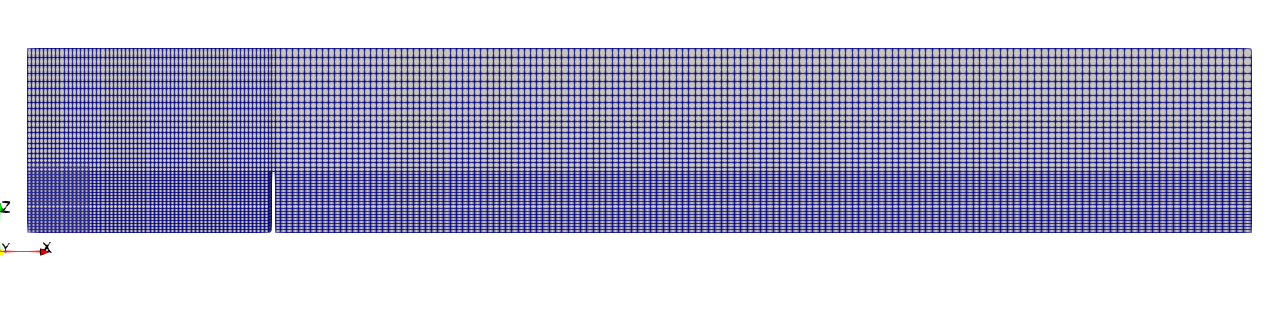
\includegraphics[width=0.9\textwidth]{images/ex1-mesh1}
	\caption{vertical flap: fluid mesh}
	\label{fig:ex1-mesh}
\end{figure}


\begin{table}[!htb]
	\begin{center}
		\begin{tabular}{ l c l | c } 
			parameter & & & value  \\ 
			\hline
			fluid density  & $\rho$ & \si{kg.m^{-3}} & 1   \\
			kinematic viscosity & $\nu$& \si{m^2.s^{-1}} & $10^{-3}$  \\
%			Reynolds length & $l_{Re}$ & $0.1$ & \si{m} \\
%			Reynolds number & Re & $\approx 1000$ & \\
			flow velocity & $\vec{v}$& \si{m.s^{-1}} & 10 \\
			flow type & & & laminar \\
		\end{tabular}
	\end{center}
	\caption{Vertical flap: fluid properties}
	\label{table:ex1-fluid}
\end{table}



\begin{table}[!htb]
	\begin{center}
		\begin{tabular}{ l c | c } 
			parameter & & value   \\ 
			\hline
			number of mesh points  & $n_{dof}$ & 17344     \\
			number of cells & $n_c$ & 8400  \\
			number of interface cells  & $n_{int}$ & 42  \\			
		\end{tabular}
	\end{center}
	\caption{Vertical flap: mesh properties}
	\label{table:ex1-mesh}
\end{table}



\subsection{Simulation and Coupling parameters}

The coupling between the fluid solver and the structural solver is the same for the MBDyn and the CalculiX simulation. The main data are given in Table \ref{table:ex1-coupling}:


\begin{table}[!htb]
	\begin{center}
		\begin{tabular}{ l c  l| c } 
			parameter & & & value   \\ 
			\hline
			simulation time  & $t$& \si{s} & 5      \\
			step size & $\Delta t$ & \si{s} & $10^{-2}$   \\
			\hline
			coupling scheme & & & serial implicit  $S\rightarrow F$  \\
			coupling algorithm & & &  IQN-ILS  \\
			displacement rel. convergence limit & & & $10^{-4}$ \\
			force rel. convergence limit &&  & $10^{-3}$  \\
      		interface mesh mapping & & & RBF  \\
			
		\end{tabular}
	\end{center}
	\caption{Vertical flap: coupling parameters}
	\label{table:ex1-coupling}
\end{table}





\subsection{Structural Solver: CalculiX}

The structural model built in CalculiX is composed of 40 \textbf{C3D8}\footnote{general purpose linear brick element with 8 nodes} as represented in Figure \ref{fig:cx-mesh}. 

\begin{figure}[htbp!]
	\centering
	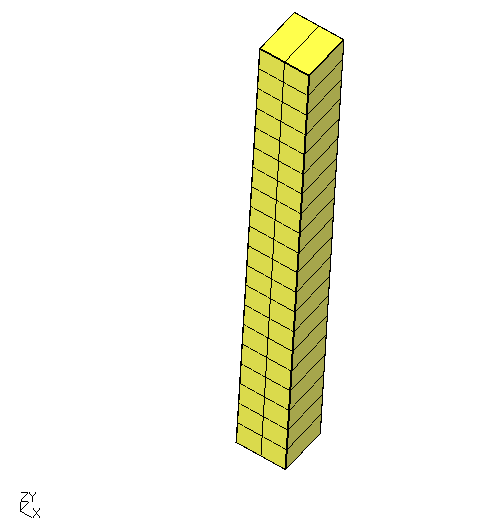
\includegraphics[width=0.6\textwidth]{images/cx1}
	\caption{vertical flap: CalculiX mesh}
	\label{fig:cx-mesh}
\end{figure}

The properties of the solid are reported in Table \ref{table:ex1-solid}.

\begin{table}[!htb]
	\begin{center}
		\begin{tabular}{ l c  l | c } 
			parameter & & value &    \\ 
			\hline
			solid density  & $\rho$ & \si{kg.m^{-3}} & 3000    \\
			Elastic modulus  & E & \si{Pa} & $4\cdot 10^6$    \\
			Poisson coefficient & $\nu$ & & $0.3$  \\
			%			Reynolds length & $l_{Re}$ & $0.1$ & \si{m} \\
			%			Reynolds number & Re & $\approx 1000$ & \\
		\end{tabular}
	\end{center}
	\caption{Vertical flap: solid properties}
	\label{table:ex1-solid}
\end{table}

 
\subsection{Implementation with MBDyn}


The MBDyn model uses the same solid properties of Table \ref{table:ex1-solid} and is composed of 10 \texttt{beam3} elements. Apart from the different orientation, the setup is the same as the one briefly described in Section \ref{sec:dummy}. The only relevant parameter that can be explicitly set up in MBDyn in comparison to CalculiX, consists in the structural damping of the beam elements (see Section \ref{sec:mbd-beam}), which is set to be proportional to stiffness matrix of the element with a coefficient of $2\cdot10^{-3}$.

The interface mesh is divided into 20 faces for the front and back surfaces of the flap. The upper surface is divided into 2, so that the interface is identical to the one obtained in CalculiX. 



\subsection{Results}

The problem considered is characterized by the adimensional parameters given in Table \ref{table:ex1-adim} and its solution is represented in Figure \ref{fig:vf_sol}.


\begin{table}[!htb]
	\begin{center}
		\begin{tabular}{ l c | r } 
			parameter & & value   \\ 
			\hline
			mass number  & $M$ & $3.3\cdot 10^{-4}$     \\
			reduced velocity & $U_R$ & $0.274$  \\
			Cauchy number  & $C_Y$ & $2.5\cdot 10^{-5}$  \\			
		\end{tabular}
	\end{center}
	\caption{Vertical flap: adimensional numbers}
	\label{table:ex1-adim}
\end{table}

\begin{figure}[htbp!]
	\centering
	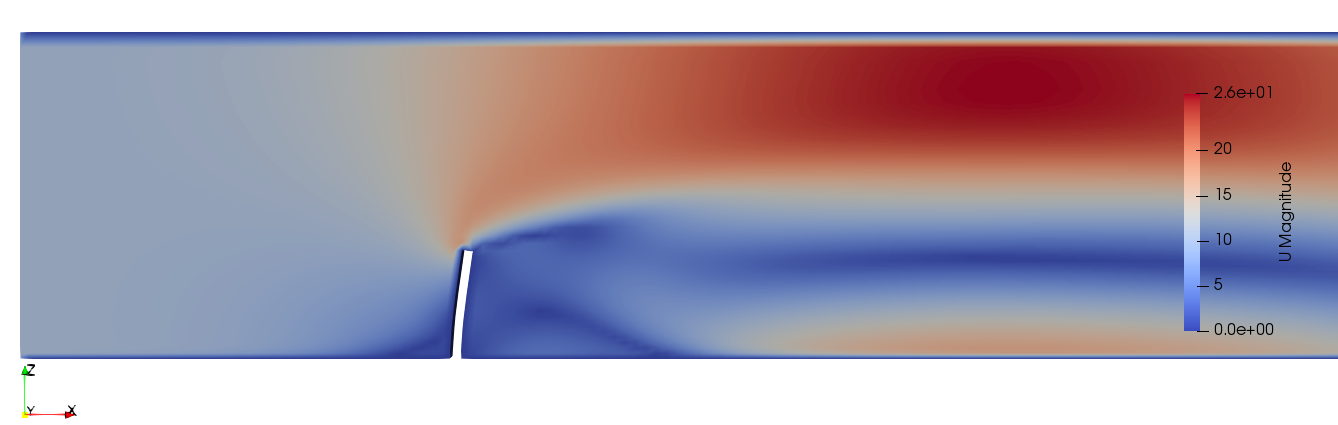
\includegraphics[width=0.9\textwidth]{images/vert_flap/vert_flap1.png}
	\caption{vertical flap: velocity field}
	\label{fig:vf_sol}
\end{figure}


The solutions between CalculiX and MBDyn are first compared in terms of resultants applied to the structure during the simulation (Figures \ref{fig:vf_force} and \ref{fig:vf_moment}), then the tip displacement in $x$ direction is considered in Figure \ref{fig:vf_displacement}. The forces and moments applied to the structure in the two cases are very close. 
The tip displacement shows that both structures exhibit the same damping and the oscillating frequency is very close: CalculiX shows a slightly higher frequency and a more visible second order frequency. The MBDyn structure looks a little more flexible: after 50 seconds of simulation tends to $58mm$ of tip displacement in $x$ direction, while the same structure in CalculiX tends to $53mm$ of displacement. 

\begin{figure}[htbp!]
	\centering
	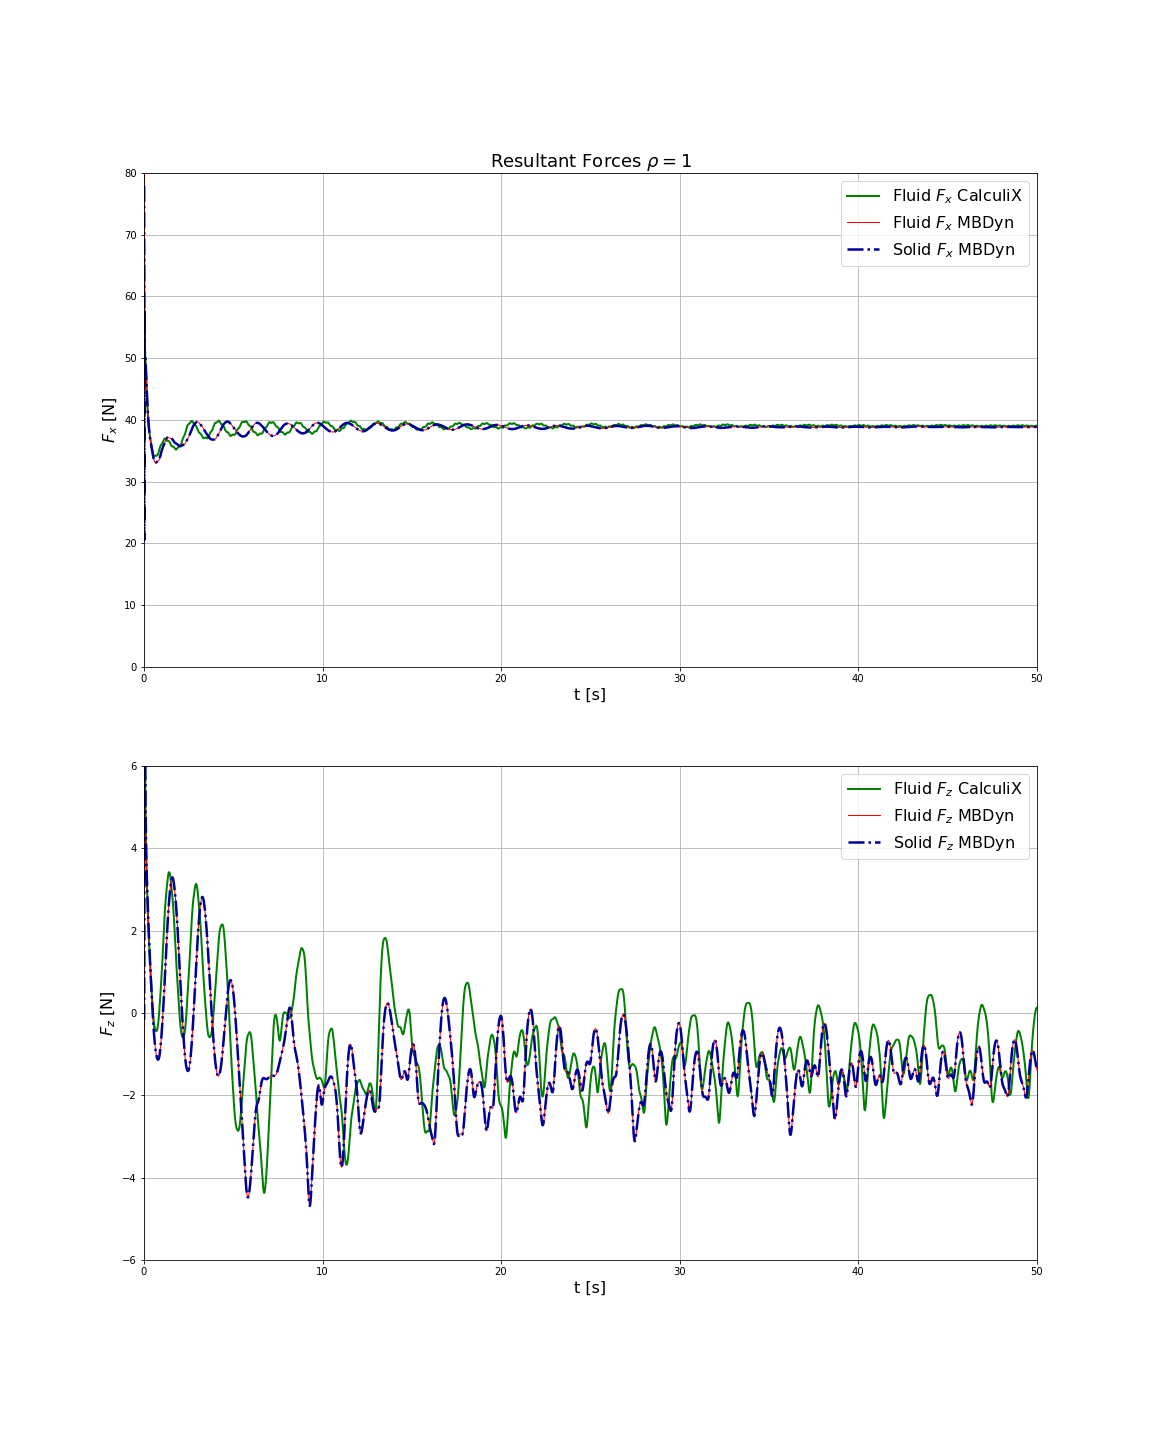
\includegraphics[width=0.9\textwidth]{images/vert_flap/forces_rho1.png}
	\caption{vertical flap: resultant forces}
	\label{fig:vf_force}
\end{figure}

\begin{figure}[htbp!]
	\centering
	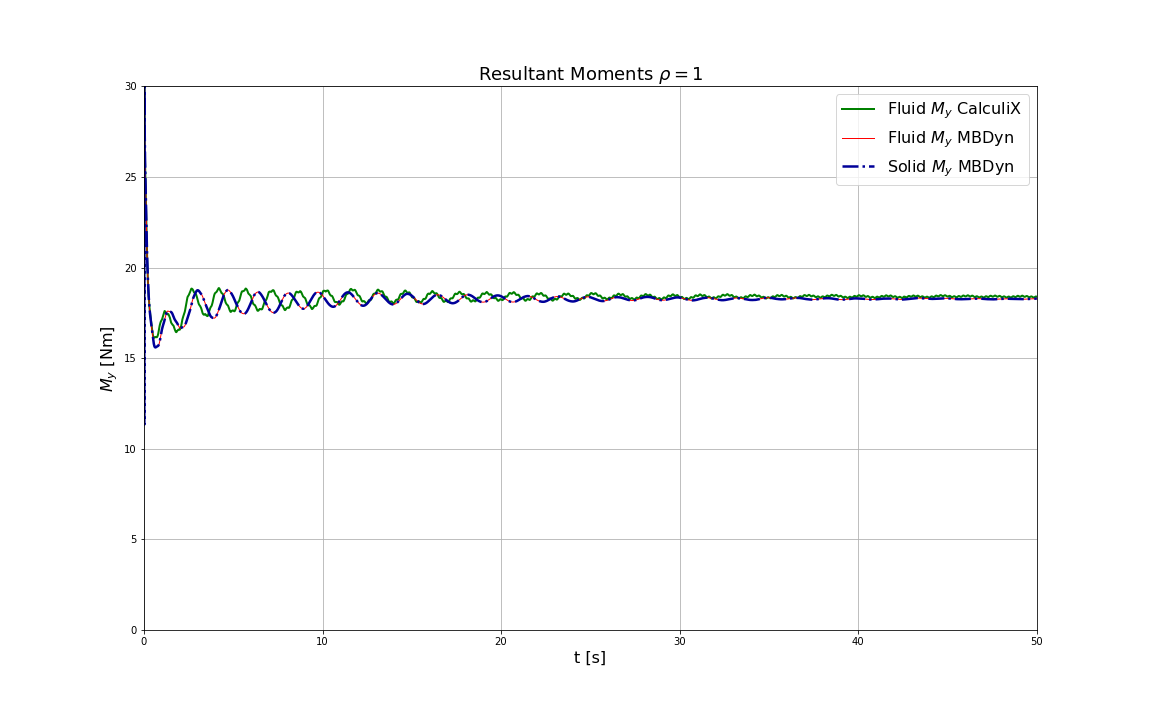
\includegraphics[width=0.9\textwidth]{images/vert_flap/moments_rho1.png}
	\caption{vertical flap: moment applied at root}
	\label{fig:vf_moment}
\end{figure}



\begin{figure}[htbp!]
	\centering
	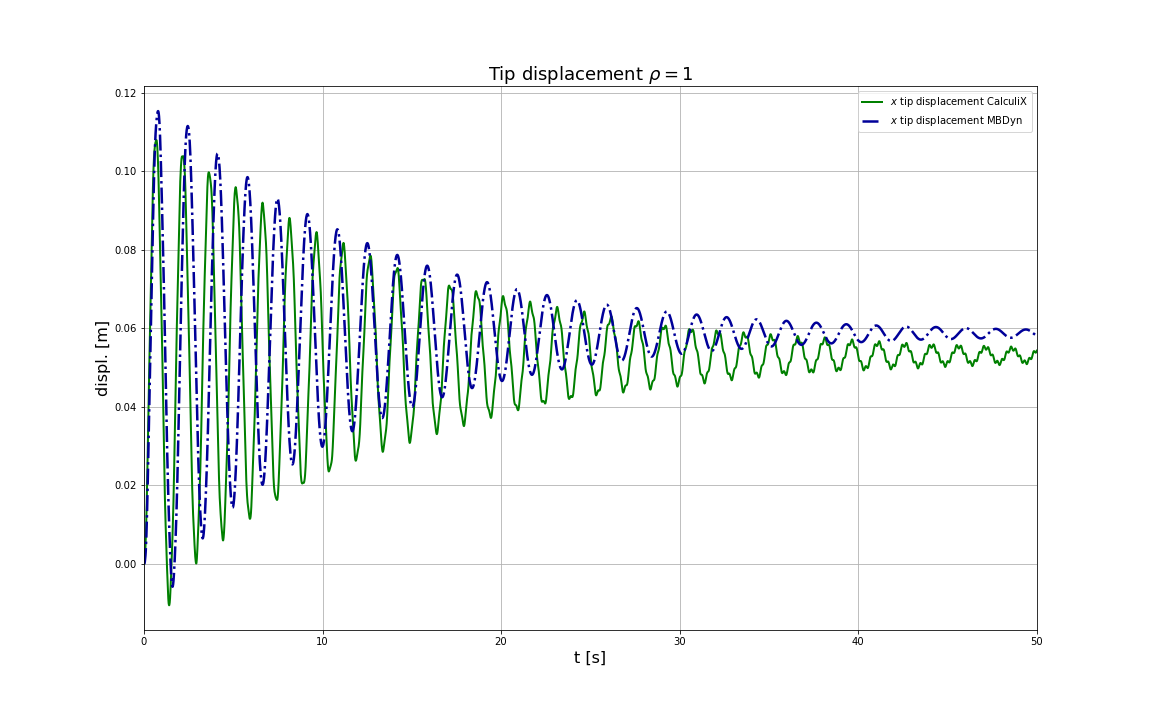
\includegraphics[width=0.9\textwidth]{images/vert_flap/disp_rho1.png}
	\caption{vertical flap: tip displacement x direction}
	\label{fig:vf_displacement}
\end{figure}


As to convergence and number of iterations between the two solvers, Figure \ref{fig:vf_cx_iter} and \ref{fig:vf_mbd_iter} show that, in general, MBdyn and CalculiX require 2 iterations to converge. This can be explained by the small mass number of this case. At some iterations MBDyn requires more iterations: this is due to the fact, for some reasons due to the coupling not completely understood at the moment, a force unbalance arises in the y-direction (out of the plane of the model) which produces a moment around x-axis. This moment is absorbed by the rotation constraints at the nodes and it does not affect the behavior of the resultant in x and z directions. 

\begin{figure}[htbp!]
	\centering
	\begin{subfigure}{0.8\textwidth}
	\centering
	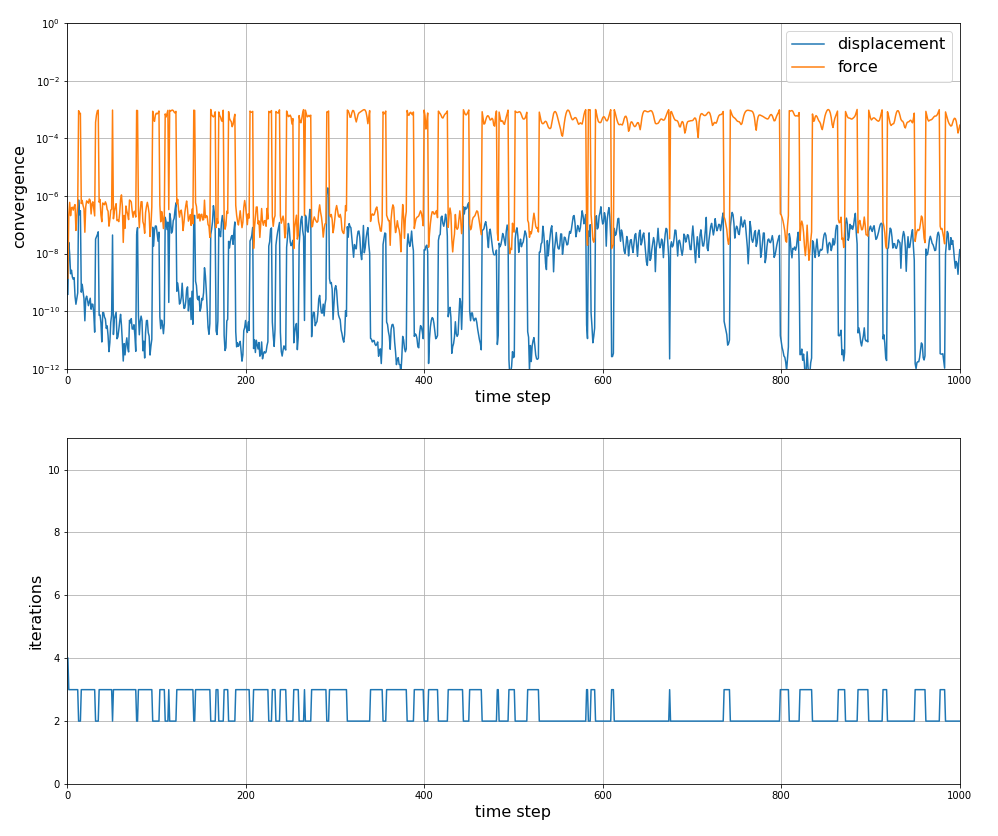
\includegraphics[width=\textwidth, trim=0 0 0 20, clip]{images/vert_flap/CX_iterations_rho1.png}
	\caption{CalculiX}
	\label{fig:vf_cx_iter}
	\end{subfigure}
	\begin{subfigure}{0.9\textwidth}
	\centering
	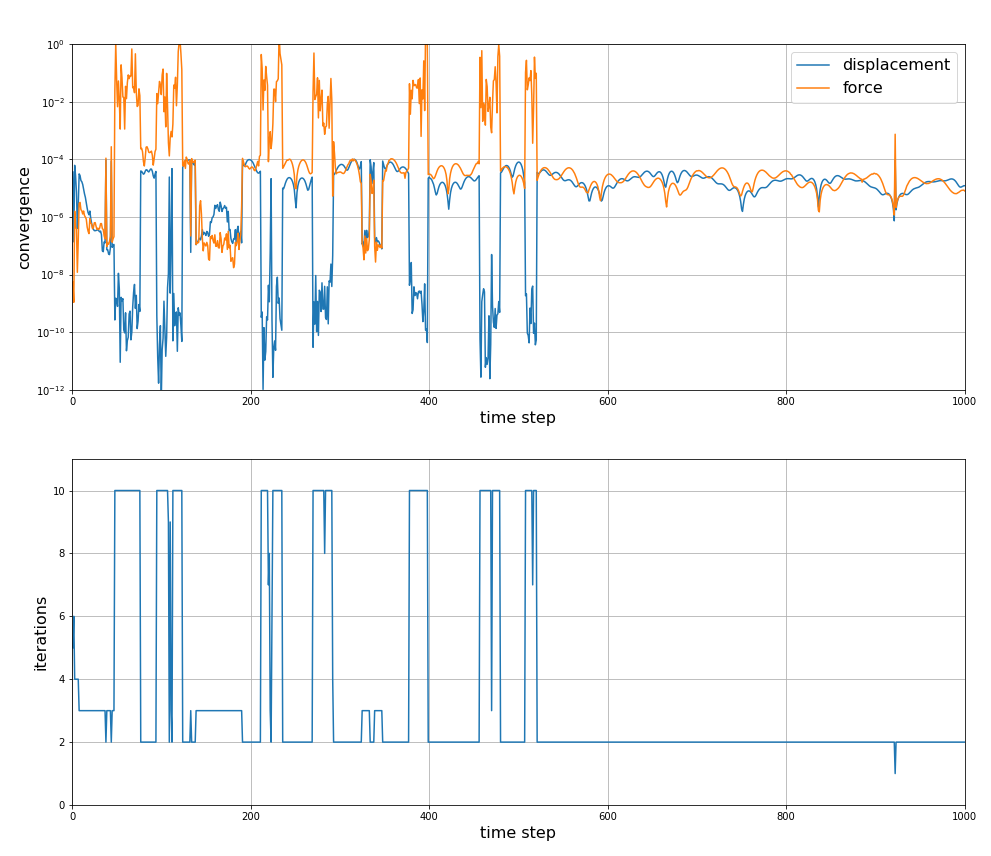
\includegraphics[width=\textwidth, trim=0 0 0 20, clip]{images/vert_flap/MBD_iterations_rho1.png}
	\caption{MBDyn}
	\label{fig:vf_mbd_iter}
	\end{subfigure}
	\caption{vertical flap: convergence and iterations}
	\label{fig:vf_iter}
\end{figure}


Finally, MBDyn allows to analyze the internal forces of each beam, as represented in Figure \ref{fig:vf_mbd_internal}.

\begin{figure}[htbp!]
	\centering
	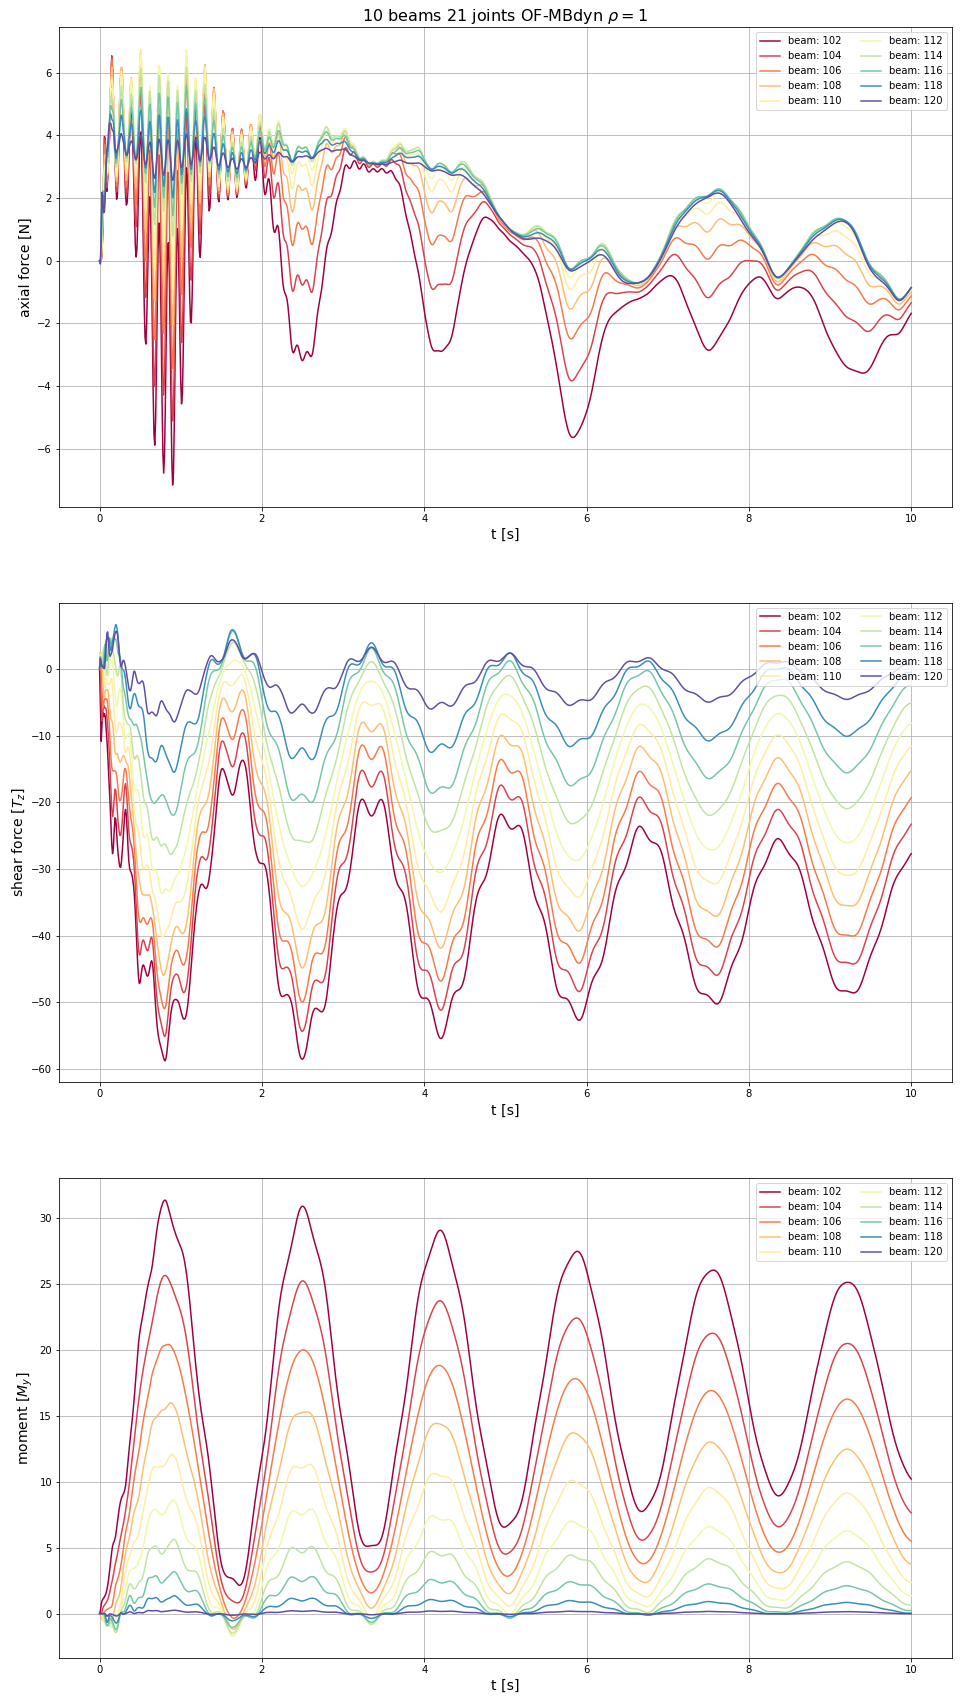
\includegraphics[width=0.82\textwidth]{images/vert_flap/OF-MBDyn_rho1_act.png}
	\caption{vertical flap: MBDyn convergence and iterations}
	\label{fig:vf_mbd_internal}
\end{figure}


\newpage

\section{Vertical flap: compressible regime}
\label{sec:su2-mbd}

A model similar to the one described in the previous section has been used to test the coupling capabilities of the adapter with a different fluid solver: SU2\footnote{\href{https://su2code.github.io/}{su2code.github.io}}. The coupling adapter between SU2 and preCICE allows to build FSI simulations in compressible regime. Besides, SU2 allows to define strictly bidimensional domains, while OpenFOAM and MBDyn are strictly tridimensional. Bidimensionality is enforced in OenFOAM using \textit{empty} boundary conditions, while in MBDyn is enforced through constraints on nodes.
For those reasons a similar model has been built. 


\subsection{Fluid domain}

The fluid domain is represented in Figure \ref{fig:comp-domain}. The inlet is on the left with uniform flow velocity, the outlet is on the right, while all other boundaries are \textit{slip} walls.


\begin{figure}[htbp!]
	\centering
	\begin{tikzpicture}
	    \pgfmathsetmacro{\xa}{-1.1}
	    \pgfmathsetmacro{\xb}{-1}
		\point{a}{-4}{0};
		\point{b}{\xa}{0};
		\point{c}{\xb}{0};
		\point{d}{8}{0};
		\point{e}{\xa}{1};
		\point{f}{\xb}{1};
		\point{g}{-4}{3};
		\point{h}{8}{3};
		
		\point{i}{-3.5}{0.5};
		
		\beam{2}{a}{b};
		\beam{2}{c}{d};
		\beam{2}{a}{g};
		\beam{2}{d}{h};
		\beam{2}{g}{h};
		\beam{4}{b}{e};
		\beam{4}{e}{f};
		\beam{4}{f}{c};
		
		\dimensioning{1}{g}{h}{3.5}[$4.2m$];
		\dimensioning{1}{a}{b}{-0.6}[$1.2m$];
		\dimensioning{2}{d}{h}{8.5}[$1.2m$];
		
		\dimensioning{1}{e}{f}{1.25}[$0.002m$];
		\dimensioning{2}{c}{f}{-0.2}[$0.4m$];
		
		\lineload{1}{a}{g};
		
		\load{1}{i}[180][1][-1];
		\load{1}{i}[-90][1][-1];
		\notation{1}{-2.5,0.25}{x};
		\notation{1}{-3.75,1.5}{y};
		%\dscaling{3}{0.4};
		%\daxis{1}{1.5 ,0 ,0}[right]][above];
	\end{tikzpicture}
	\caption{vertical flap (compressible): fluid domain}
	\label{fig:comp-domain}
\end{figure}


The fluid domain is discretized in an unstructured triangular mesh as depicted in Figure \ref{fig:comp-mesh}. The main fluid and mesh values are given in Table \ref{table:comp-fluid} and \ref{table:comp-mesh}. 

\begin{figure}[htbp!]
	\centering
	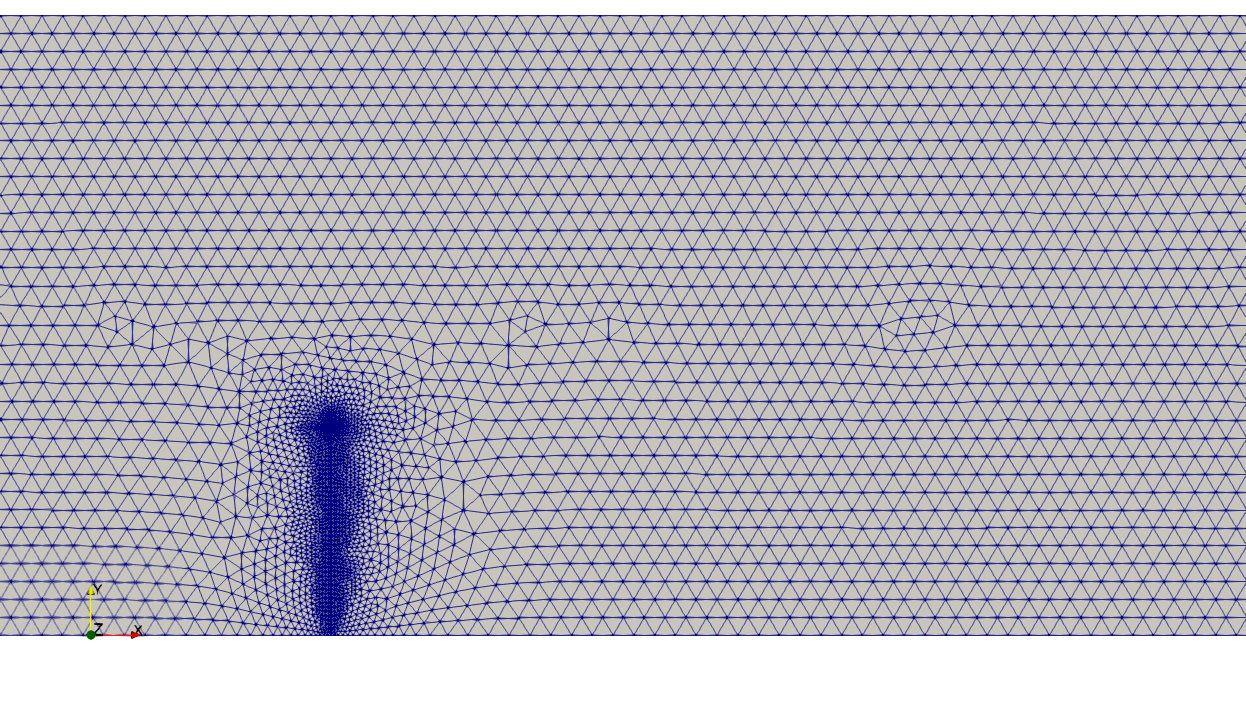
\includegraphics[width=0.9\textwidth, trim=0 100 0 100,clip]{images/comp_flap/mesh.png}
	\caption{vertical flap (compressible): fluid mesh}
	\label{fig:comp-mesh}
\end{figure}


\begin{table}[!htb]
	\begin{center}
		\begin{tabular}{ l c l | c } 
			parameter & & & value  \\ 
			\hline
			fluid properties  &  &  & standard air   \\
			outlet pressure & $p$& \si{Pa} & $101300$  \\
			inlet temperature & $T$ & \si{K} & 288  \\
%			Reynolds number & Re & $\approx 1000$ & \\
			inlet Mach number &  Ma &  & 0.1 \\
			flow type & & & euler \\
		\end{tabular}
	\end{center}
	\caption{Vertical flap (compressible): fluid properties}
	\label{table:comp-fluid}
\end{table}



\begin{table}[!htb]
	\begin{center}
		\begin{tabular}{ l c | c } 
			parameter & & value   \\ 
			\hline
			number of mesh points  & $n_{dof}$ & 5580     \\
			number of cells & $n_c$ & 10709  \\
			number of interface points  & $n_{int}$ & 162  \\			
		\end{tabular}
	\end{center}
	\caption{Vertical flap (compressible): mesh properties}
	\label{table:comp-mesh}
\end{table}


\subsection{MBDyn model}


The MBDyn model uses solid properties defined in Table \ref{table:comp-solid} and is composed of 5 \texttt{beam3} elements. 

\begin{table}[!htb]
	\begin{center}
		\begin{tabular}{ l c  l | c } 
			parameter & & & value   \\ 
			\hline
			solid density  & $\rho$ & \si{kg.m^{-3}} & 1000    \\
			Elastic modulus  & E & \si{Pa} & $ 5.6 \cdot 10^9$    \\
			Poisson coefficient & $\nu$ & & $0.4$  \\
			structural damping & & & $1 \cdot 10^{-3}$ \\
			%			Reynolds length & $l_{Re}$ & $0.1$ & \si{m} \\
			%			Reynolds number & Re & $\approx 1000$ & \\
		\end{tabular}
	\end{center}
	\caption{Vertical flap: solid properties}
	\label{table:comp-solid}
\end{table}

\subsection{Coupling parameters}

The main data concerning the coupling between MBDyn and SU2 are given in Table \ref{table:comp-coupling}:

\begin{table}[!htb]
	\begin{center}
		\begin{tabular}{ l c  l| c } 
			parameter & & & value   \\ 
			\hline
			simulation time  & $t$& \si{s} & 1      \\
			step size & $\Delta t$ & \si{s} & $10^{-3}$   \\
			\hline
			coupling scheme & & & serial implicit $S\rightarrow F$  \\
			coupling algorithm & & &  IQN-ILS  \\
			displacement rel. convergence limit & & & $10^{-5}$ \\
			force rel. convergence limit &&  & $10^{-3}$  \\
      		interface mesh mapping & & & RBF  \\
			
		\end{tabular}
	\end{center}
	\caption{Vertical flap (compressible): coupling parameters}
	\label{table:comp-coupling}
\end{table}


\subsection{Results}

The problem considered is characterized by the adimensional parameters given in Table \ref{table:comp-adim}: in particular the mass number remains in the order of $\mathcal{O} \left(10^{-3}\right)$. A sketch of the flow solution is represented in Figure \ref{fig:comp_sol}.

\begin{table}[!htb]
	\begin{center}
		\begin{tabular}{ l c | r } 
			parameter & & value   \\ 
			\hline
			mass number  & $M$ & $ \approx 1.2\cdot 10^{-3}$     \\
			reduced velocity & $U_R$ & $ \approx 1.44\cdot 10^{-2}$  \\
			Cauchy number  & $C_Y$ & $  \approx 2.53 \cdot 10^{-7}$  \\			
		\end{tabular}
	\end{center}
	\caption{Vertical flap (compressible): adimensional numbers}
	\label{table:comp-adim}
\end{table}

\begin{figure}[htbp!]
	\centering
	\begin{subfigure}{0.9\textwidth}
	\centering
	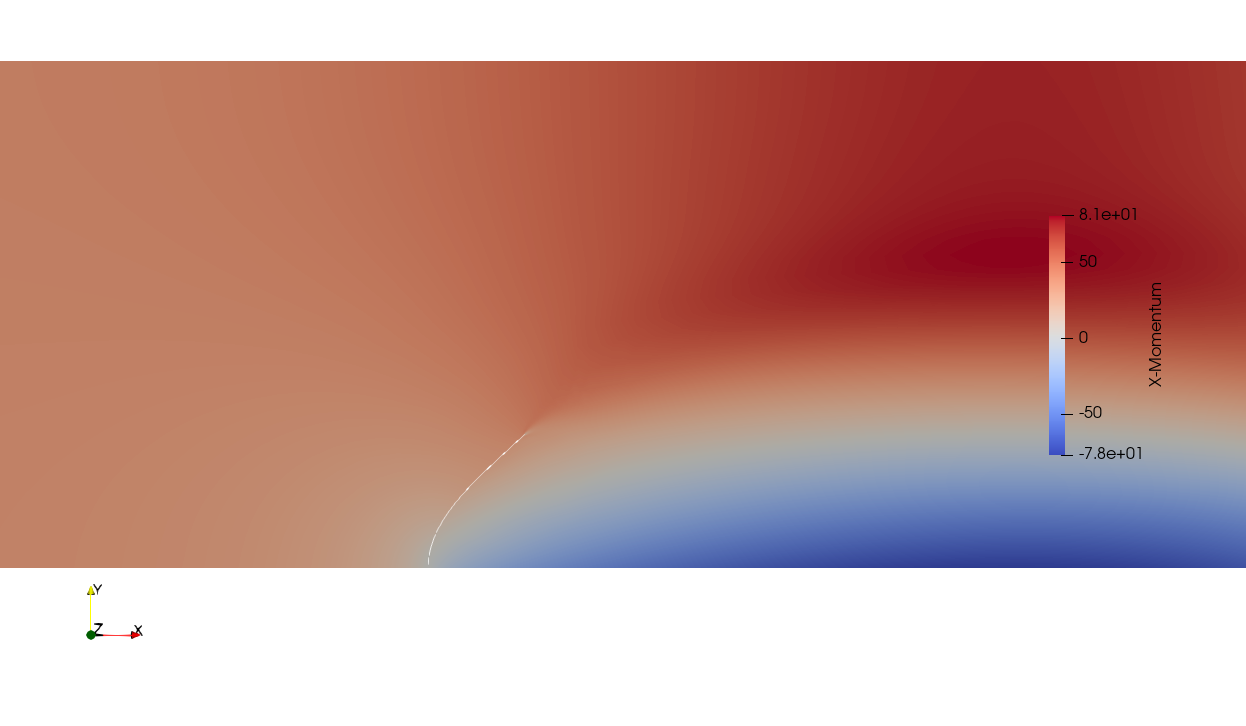
\includegraphics[width=\textwidth, trim=0 150 0 150, clip]{images/comp_flap/x-mom.png}
	\caption{vertical flap (compressible): x-momentum}
	\end{subfigure}
	\begin{subfigure}{\textwidth}
	\centering
	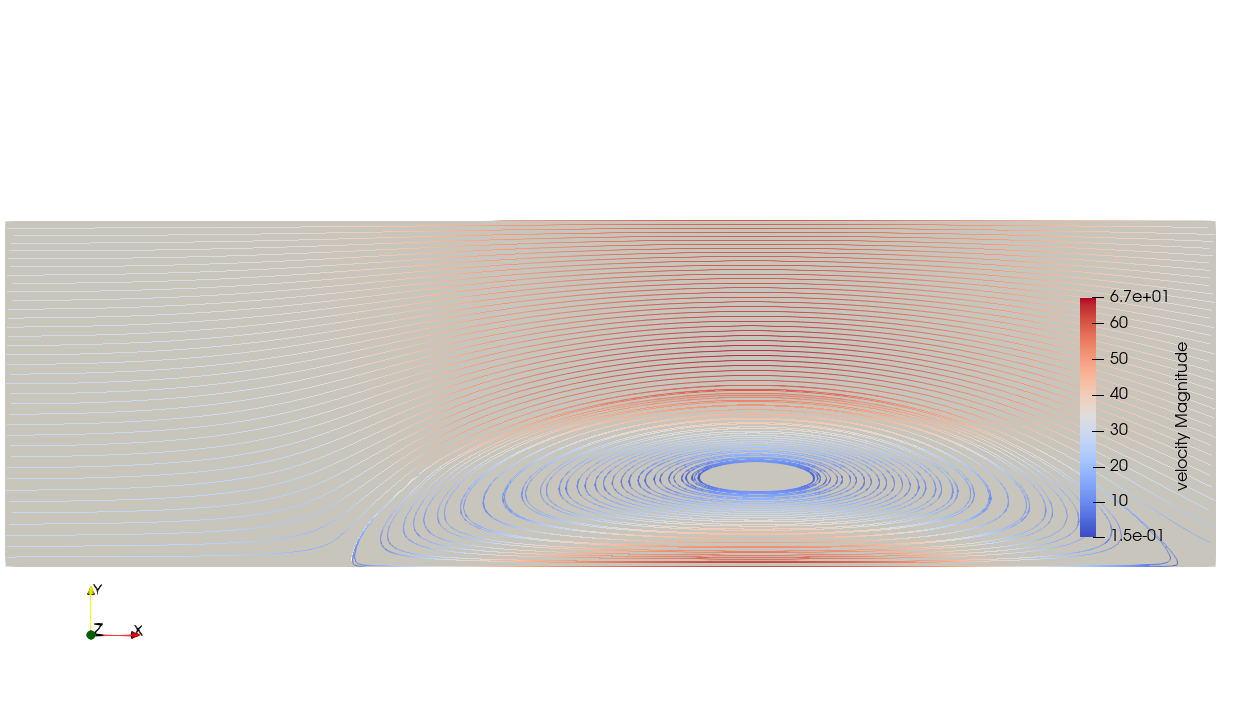
\includegraphics[width=0.95\textwidth, trim=0 150 0 150, clip]{images/comp_flap/vel-stream.png}
	\caption{vertical flap (compressible): streamlines}
	\end{subfigure}
	\caption{vertical flap (compressible): flow solution}
	\label{fig:comp_sol}
\end{figure}


The combination of parameters considered in this test case aimed at considering a very thin flexible element surrounded by a low-Mach flow, so that large displacements are involved. The structure reaches a steady deformed shape after around 1 second as shown in Figure  \ref{fig:comp_displacement}, concerning tip displacement. 

The fluid flow has been initialized with a steady solution obtained considering a rigid structure, then the FSI problem has been simulated applying the the aerodynamic load to the flap progressively: a linear ramp starting at $1\%$ of the load with a duration of 0.2 seconds (see Section \ref{sec:mbdyn-adapter-input} for the adapter input parameters).

Resultant forces $(R_x, R_y)$ and moment $(M_z)$ computed at the root of the flap are shown in Figure \ref{fig:comp_force}.

\begin{figure}[htbp!]
	\centering
	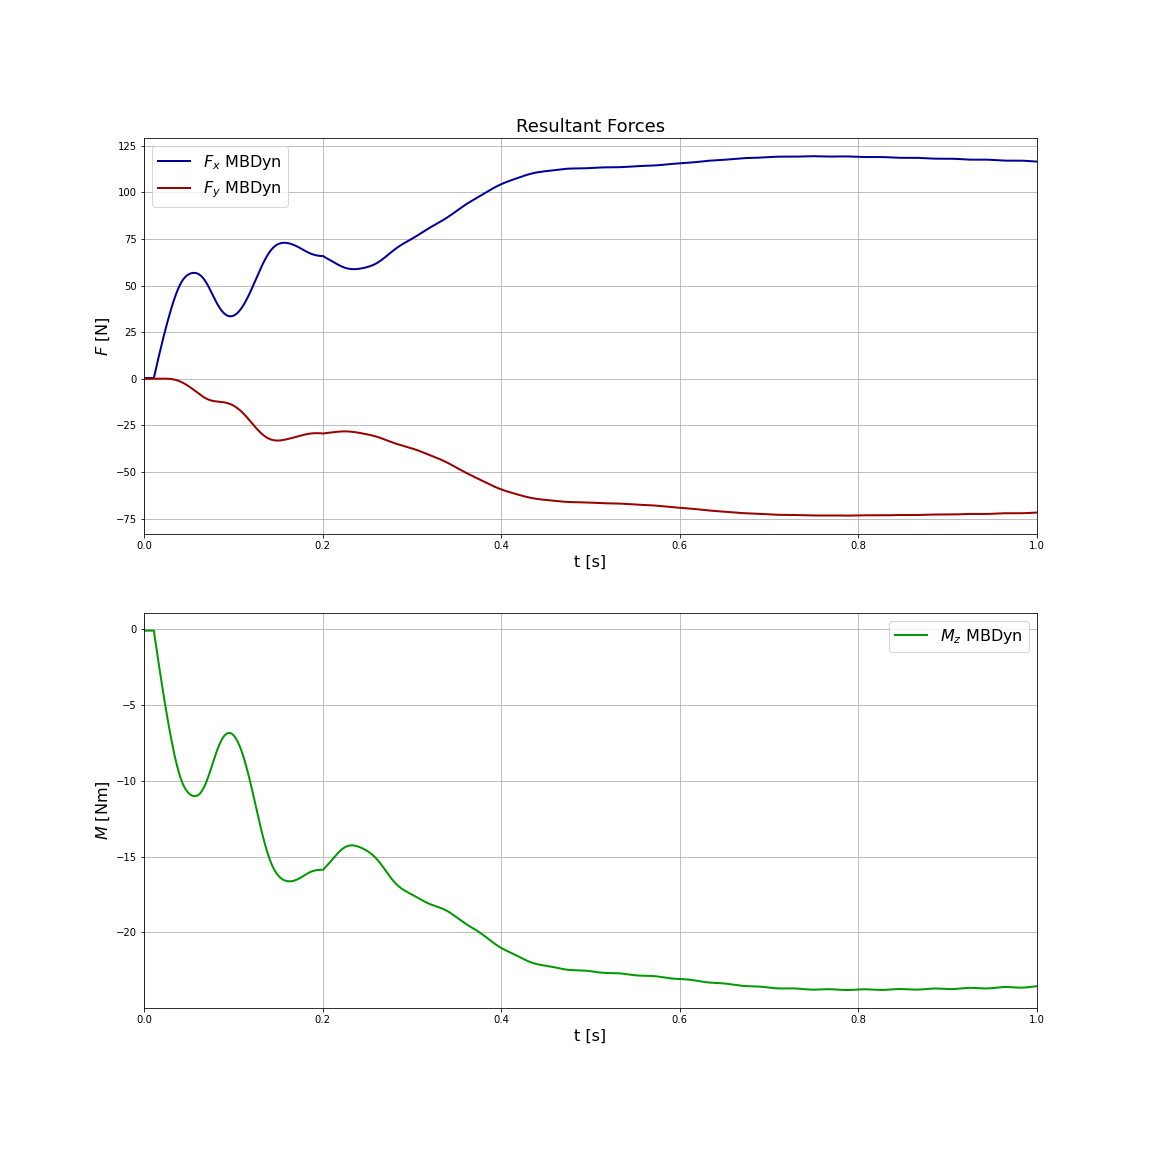
\includegraphics[width=0.9\textwidth, trim=0 100 0 100, clip]{images/comp_flap/forces_comp.png}
	\caption{vertical flap (compressible): resultant forces}
	\label{fig:comp_force}
\end{figure}



\begin{figure}[htbp!]
	\centering
	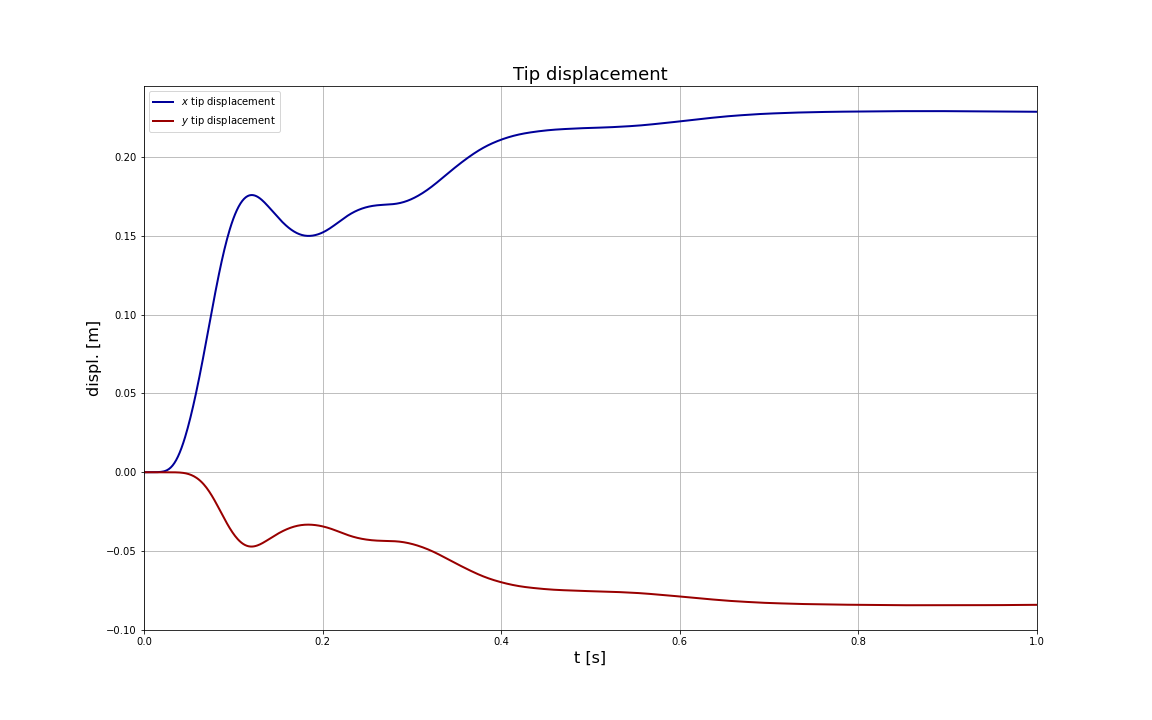
\includegraphics[width=0.9\textwidth, trim=0 50 0 50, clip]{images/comp_flap/disp_comp.png}
	\caption{vertical flap (compressible): tip displacement}
	\label{fig:comp_displacement}
\end{figure}


Each time step of the problem converges quite rapidly, requiring 5 iterations in most cases (see Figure \ref{fig:comp_mbd_iter}. This outcome agrees with the fact that a low mass number and a high fluid velocity make the problem loosely coupled (see section \ref{sec:strong-coupling} for some details). Nevertheless an explicit simulation diverges immediately.  


\begin{figure}[htbp!]
	\centering
	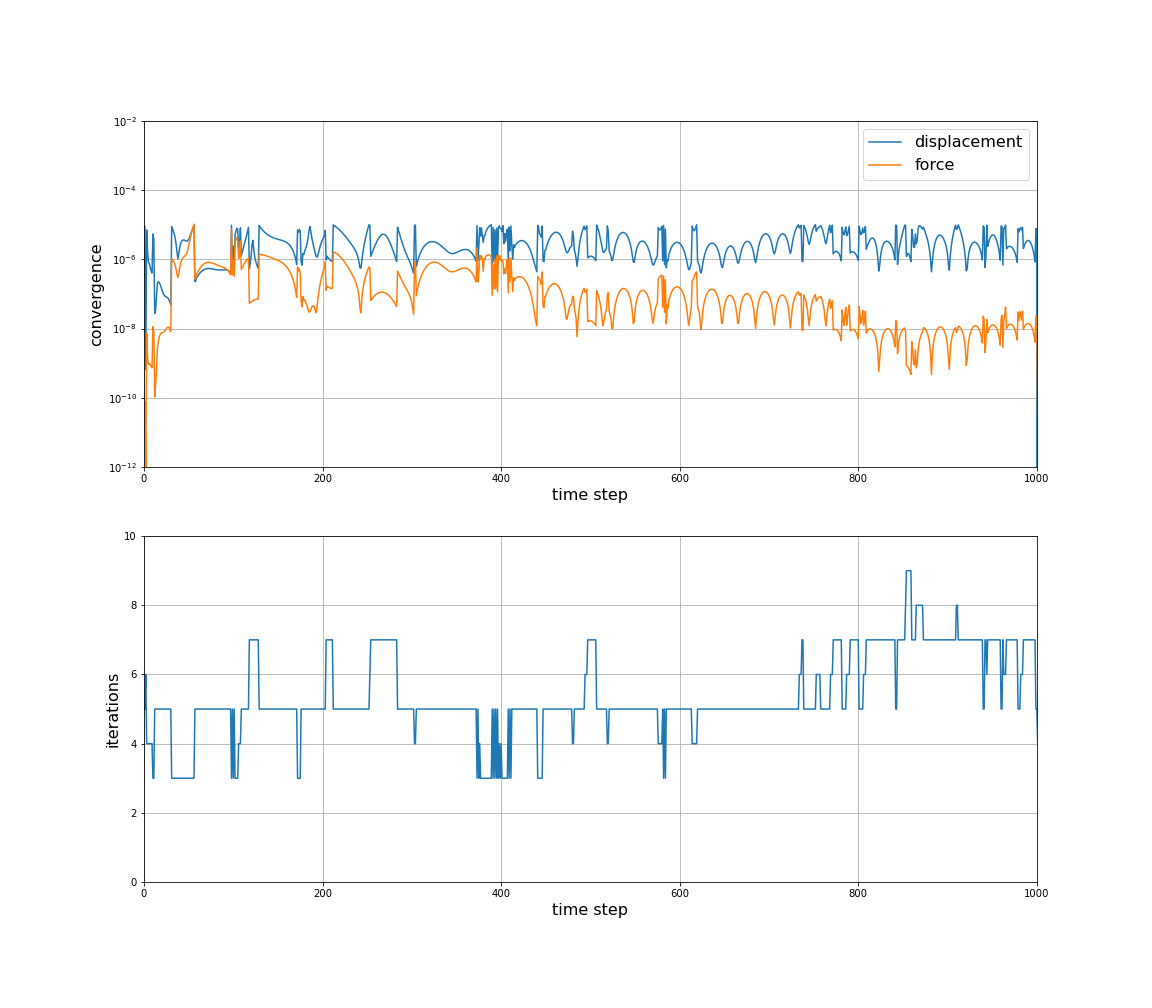
\includegraphics[width=0.95\textwidth, trim=0 80 0 100, clip]{images/comp_flap/MBD_iterations_comp.png}
	\caption{vertical flap (compressible): convergence and iterations}
	\label{fig:comp_mbd_iter}
\end{figure}

Axial, shear and bending moment in each of the MBDyn elements are plotted in Figure \ref{fig:comp_mbd_internal}.

\begin{figure}[htbp!]
	\centering
	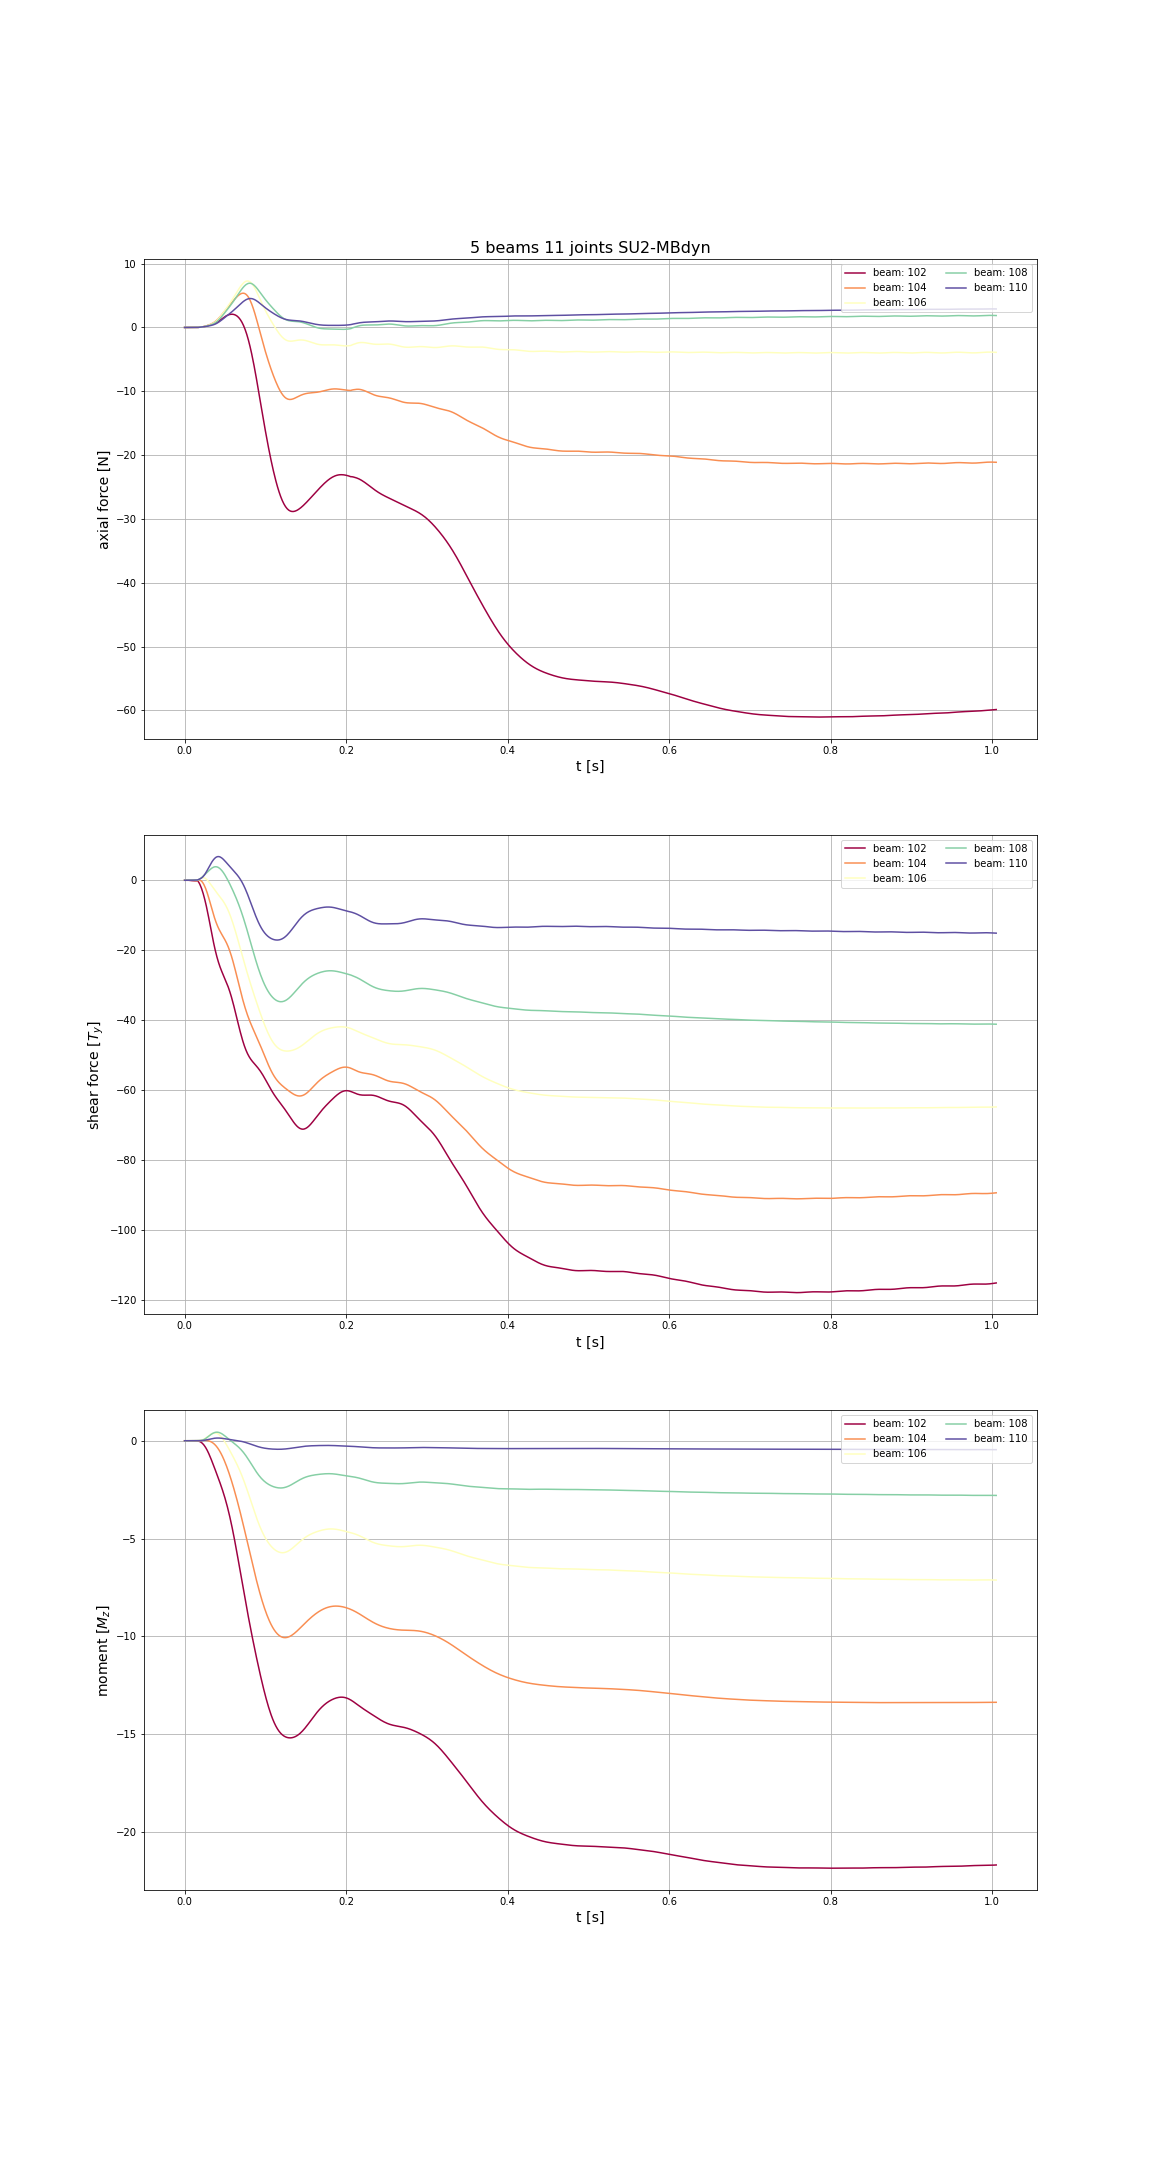
\includegraphics[width=0.92\textwidth, trim=0 230 0 230, clip]{images/comp_flap/vert-flap_SU2-MBDyn_act.png}
	\caption{vertical flap (compressible): MBDyn internal forces}
	\label{fig:comp_mbd_internal}
\end{figure}


\newpage


\section{Square bluff body Benchmark}
\label{sec:sq-cyl-bench}

The first simple problems aimed at verifying that the complete FSI problem: i.e. the MBDyn model, the mapping with the interface mesh, the coupling adapter and the fluid model (fluid flow and mesh movement performed with different solvers) is working and gives correct results.

After that it is important to verify the performance of the system considering well-known benchmarks, so that the results can be compared with a large number of algorithms and techniques.

\subsection{Problem description}

The first benchmark considered here has been described in \cite{ramm1998fluid}. The structural part is composed of a square bluff body with a trailing thin flap, as described in Figure \ref{fig:sq_domain}. The geometrical data are given in Table \ref{table:sq-geom}.

\begin{table}[!htb]
	\begin{center}
		\begin{tabular}{ l c | r } 
			parameter & & value   \\ 
			\hline
			H  & [\si{mm}] & $10$     \\
			L & [\si{mm}] & $40$  \\
			t  & [\si{mm}] & $0.6$  \\			
		\end{tabular}
	\end{center}
	\caption{square bluff body: geometry}
	\label{table:sq-geom}
\end{table}

\begin{figure}[htbp!]
	\centering
	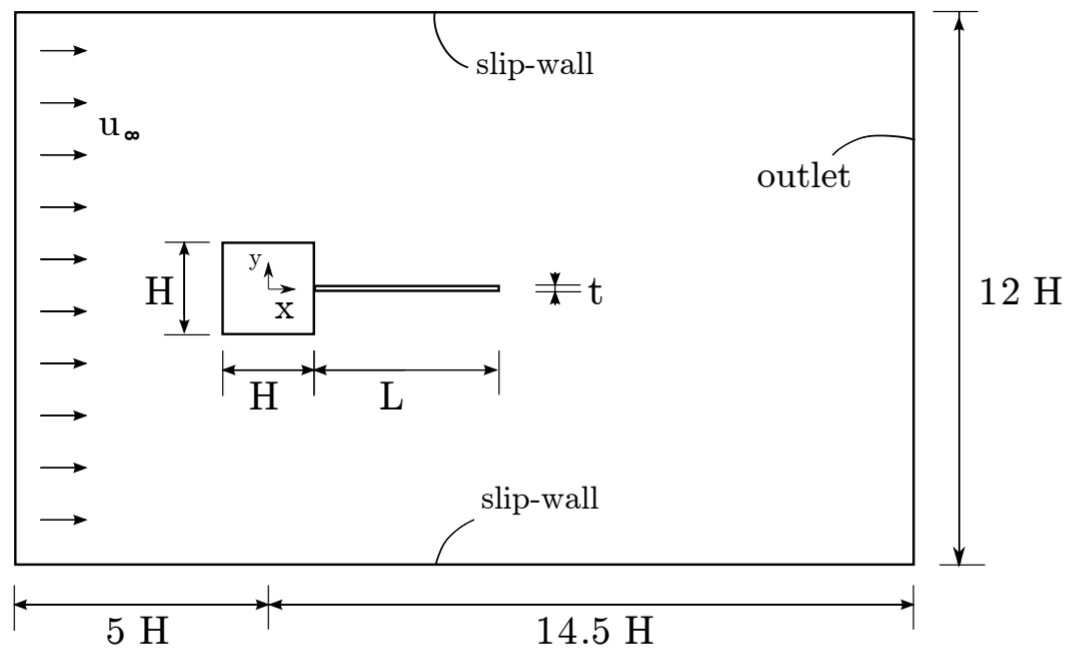
\includegraphics[width=0.82\textwidth, trim=0 0 0 0, clip]{images/sq-cyl/sq-cyl-domain.png}
	\caption{square bluff body benchmark: domain}
	\label{fig:sq_domain}
\end{figure}

\subsection{Fluid domain}

The fluid domain is represented in Figure \ref{fig:sq_domain} and has been simulated in OpenFOAM. The inlet is on the left with uniform flow velocity, the outlet is on the right, the external boundaries (top and bottom) are \textit{slip-walls} while all other boundaries (cylinder and flap) are \textit{no-slip} walls.


The fluid domain is discretized in an structured hexaedral mesh as depicted in Figure \ref{fig:sq_mesh}. The main fluid and mesh values are given in Table \ref{table:sq-fluid} and \ref{table:sq-mesh}. 

\begin{figure}[htbp!]
	\centering
	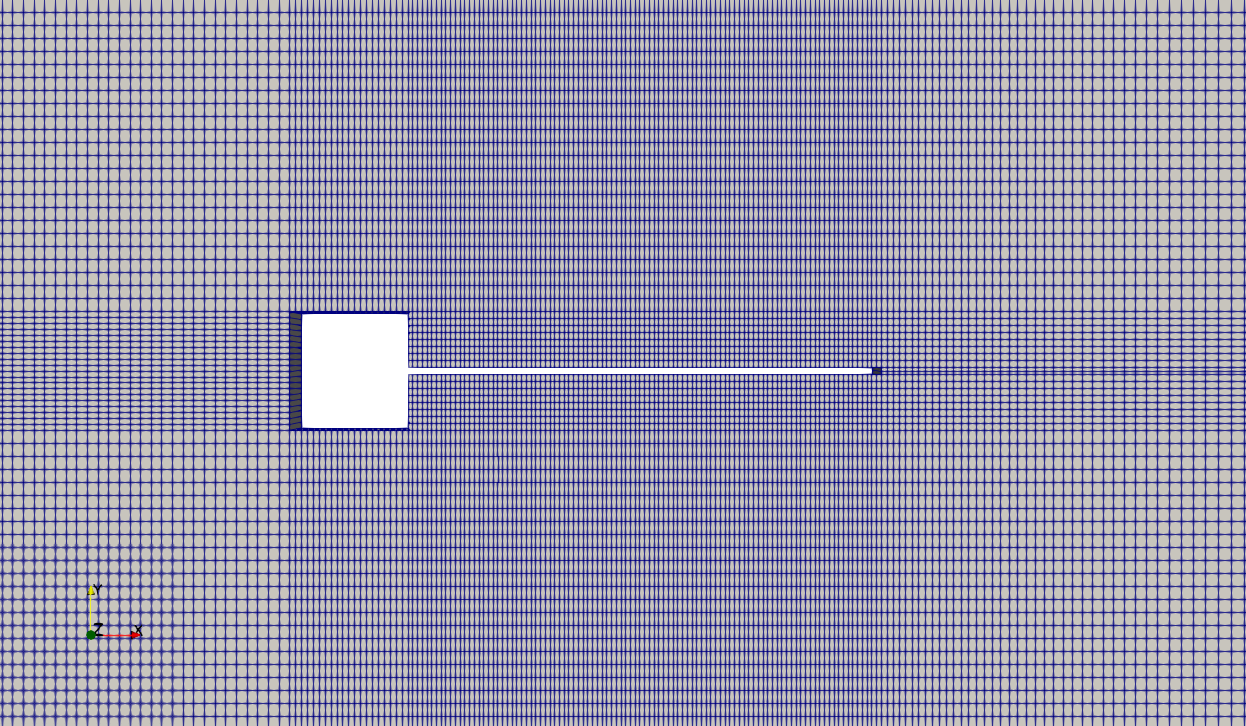
\includegraphics[width=0.9\textwidth]{images/sq-cyl/sq_mesh.png}
	\caption{square bluff body: fluid mesh}
	\label{fig:sq_mesh}
\end{figure}


\begin{table}[!htb]
	\begin{center}
		\begin{tabular}{ l c l | c } 
			parameter & & & value  \\ 
			\hline
			fluid density  & $\rho$ & \si{kg.m^{-3}} & $1.18$   \\
			dynamic viscosity & $\mu$& \si{kg.m^{-1}.s^{-1}} & $1.82 \cdot 10^{-5}$  \\
%			Reynolds length & $l_{Re}$ & $0.1$ & \si{m} \\
			Reynolds number & Re &  & $332$ \\
			flow velocity & $\vec{u}_{\infty}$ & \si{m.s^{-1}} & $0.513$ \\
			flow type & & & laminar \\
		\end{tabular}
	\end{center}
	\caption{square bluff body: fluid properties}
	\label{table:sq-fluid}
\end{table}



\begin{table}[!htb]
	\begin{center}
		\begin{tabular}{ l c | c } 
			parameter & & value   \\ 
			\hline
			number of mesh points  & $n_{dof}$ & 59096     \\
			number of cells & $n_c$ & 29040  \\
			number of interface cells  & $n_{int}$ & 202  \\			
		\end{tabular}
	\end{center}
	\caption{square bluff body: mesh properties}
	\label{table:sq-mesh}
\end{table}


\subsection{Solid domain}

The properties of the solid are reported in Table \ref{table:sq-solid}.

\begin{table}[!htb]
	\begin{center}
		\begin{tabular}{ l c  l | c } 
			parameter & & value &    \\ 
			\hline
			solid density  & $\rho$ & \si{kg.m^{-3}} & 100    \\
			Elastic modulus  & E & \si{Pa} & $2.5\cdot 10^5$    \\
			Poisson coefficient & $\nu$ & & $0.35$  \\
			%			Reynolds length & $l_{Re}$ & $0.1$ & \si{m} \\
			%			Reynolds number & Re & $\approx 1000$ & \\
		\end{tabular}
	\end{center}
	\caption{square bluff body: solid properties}
	\label{table:sq-solid}
\end{table}

The MBDyn model is composed of 10 \texttt{beam3} elements. The setup resembles the one briefly described in Section \ref{sec:dummy}. The structural damping of the beam elements (see Section \ref{sec:mbd-beam}) has been set to be proportional to stiffness matrix of the element with a coefficient of $1\cdot10^{-2}$. This value appeared to be high enough to give a smooth structural solution without being excessively damping.

The interface mesh is divided into 202 faces and is shown in Figure \ref{fig:sq_struct_mesh}. 

\begin{figure}[htbp!]
	\centering
	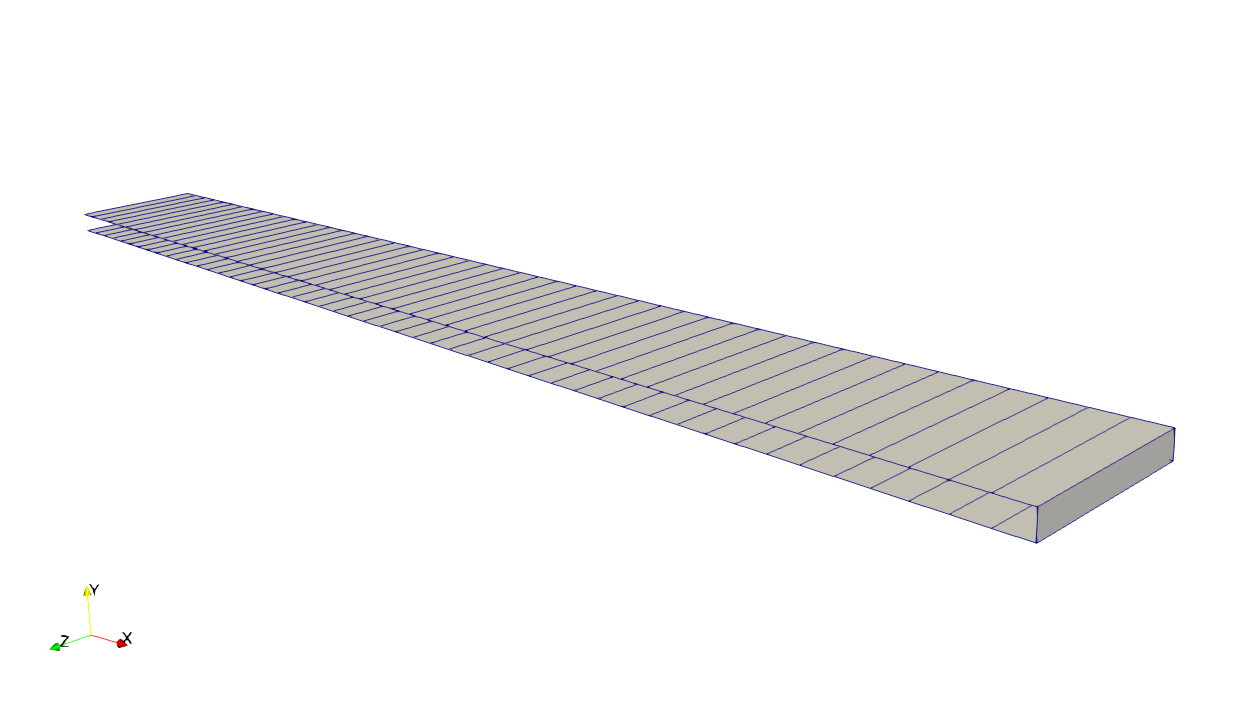
\includegraphics[width=0.9\textwidth, trim=0 50 0 200, clip]{images/sq-cyl/sq_struct_mesh.png}
	\caption{square bluff body: structural interface mesh}
	\label{fig:sq_struct_mesh}
\end{figure}


\subsection{Coupling parameters}


The main coupling data are given in Table \ref{table:sq-coupling}. The particularly short time step is required by fluid mesh movement: as it will be apparent in the results, the thin flexible flap moves quickly and with large displacement. The diffusion algorithm used by OpenFOAM to deform the fluid mesh produced inconsistent cell volumes when using higher time steps. 

\begin{table}[!htb]
	\begin{center}
		\begin{tabular}{ l c  l| c } 
			parameter & & & value   \\ 
			\hline
			simulation time  & $t$& \si{s} & 6      \\
			step size & $\Delta t$ & \si{s} & $5 \cdot 10^{-4}$   \\
			\hline
			coupling scheme & & & serial implicit  $S\rightarrow F$  \\
			coupling algorithm & & &  IQN-ILS  \\
			displacement rel. convergence limit & & & $10^{-4}$ \\
			force rel. convergence limit &&  & $10^{-3}$  \\
      		interface mesh mapping & & & RBF  \\
			
		\end{tabular}
	\end{center}
	\caption{square bluff body: coupling parameters}
	\label{table:sq-coupling}
\end{table}

Most parameters are similar to the ones used in other examples as they turned out to fit well with most of the experiments. 

\subsection{Results}

The problem considered is characterized by the adimensional parameters given in Table \ref{table:sq-adim} and its solution is represented in Figure \ref{fig:sq_sol}.

\begin{table}[!htb]
	\begin{center}
		\begin{tabular}{ l c | r } 
			parameter & & value   \\ 
			\hline
			mass number  & $M$ & $ 1.18\cdot 10^{-2}$     \\
			reduced velocity & $U_R$ & $ \approx 1\cdot 10^{-2}$  \\
			Cauchy number  & $C_Y$ & $  1.24 \cdot 10^{-6}$  \\			
		\end{tabular}
	\end{center}
	\caption{square bluff body: adimensional numbers}
	\label{table:sq-adim}
\end{table}

As in other simulations, fluid forces are applied with a ramp to ease convergence at the beginning of the simulation: during the first $100$ \si{ms} they are scaled to $10\%$ to reach $100\%$ after another $100$ \si{ms}.

Alternating vortices begin developing quite rapidly and the structure begins oscillating. After around 2 seconds reaches a vortex lock-in regime (e.g. \cite{hong2001fluid}), as shown in Figure \ref{fig:sq_displacement} (in particular the tip displacement in \textit{y} direction).



\begin{figure}[htbp!]
	\centering
	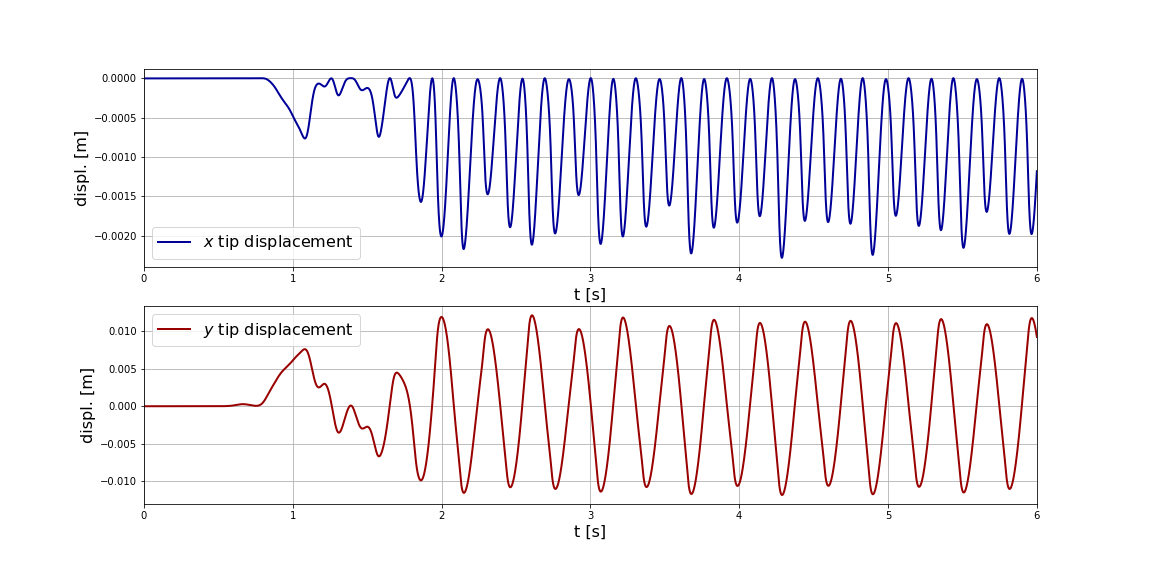
\includegraphics[width=0.98\textwidth, trim=20 20 20 50, clip]{images/sq-cyl/disp_sq.png}
	\caption{square bluff body: tip displacement}
	\label{fig:sq_displacement}
\end{figure}

Forces are measured on the whole structure on the fluid side, while are measured on the flap in the solid domain. Figure \ref{fig:sq_force} shows a detail of $0.5$ \si{s} of simulation. The difference in \textit{x}-direction represents the drag force on the cylinder. Differences in lift and moment are almost zero. 

\begin{figure}[htbp!]
	\centering
	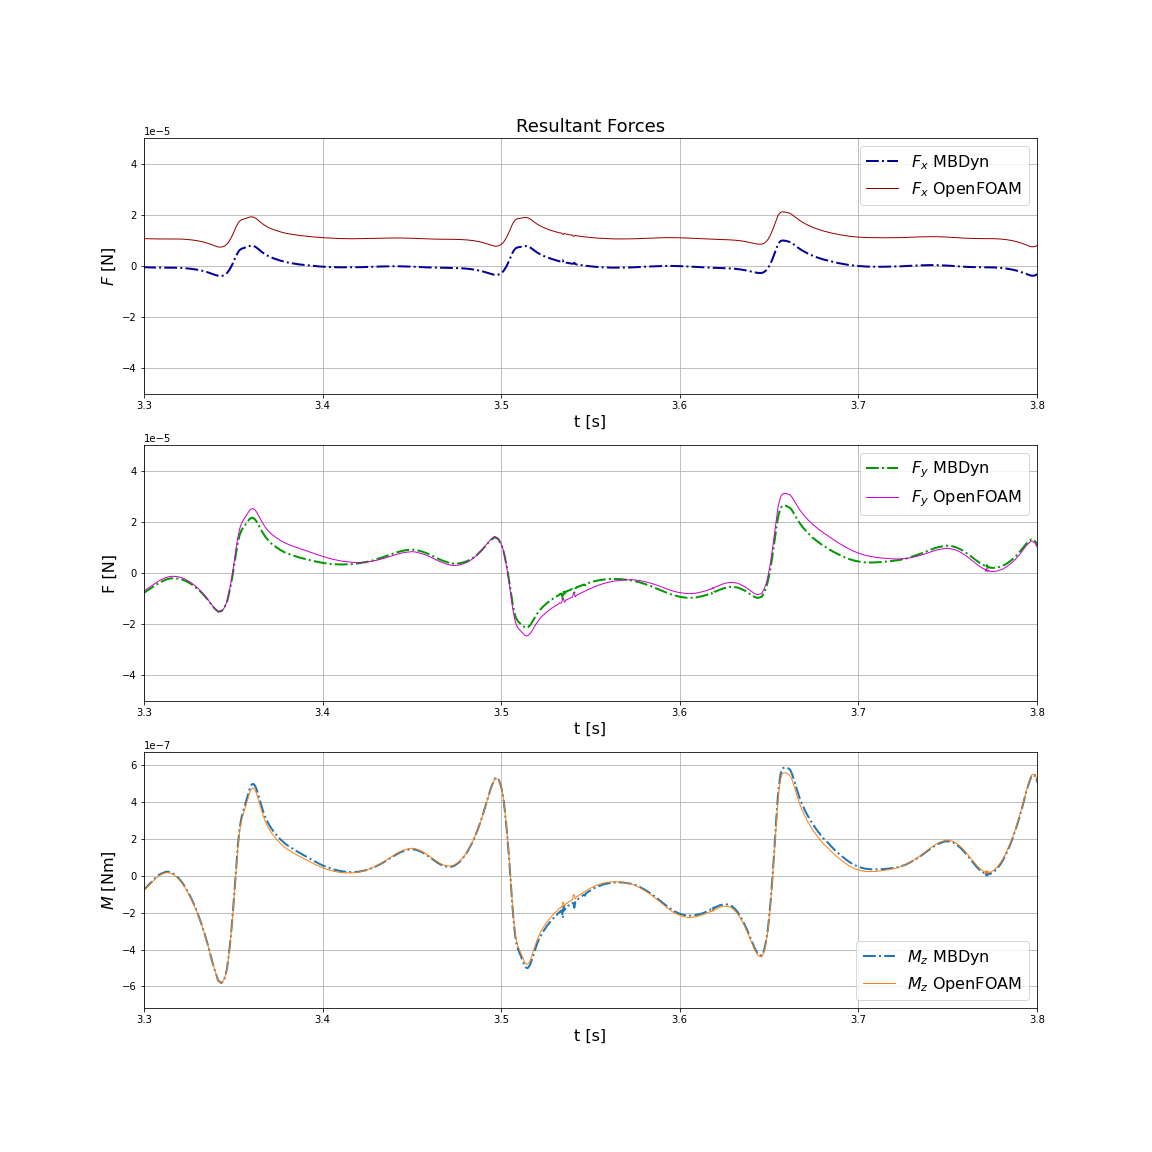
\includegraphics[width=0.98\textwidth, trim=20 100 20 100, clip]{images/sq-cyl/forces_sq.png}
	\caption{square bluff body: resultant forces (detail)}
	\label{fig:sq_force}
\end{figure}


\begin{figure}[htb]
\centering % <-- added
\begin{subfigure}{0.5\textwidth}
  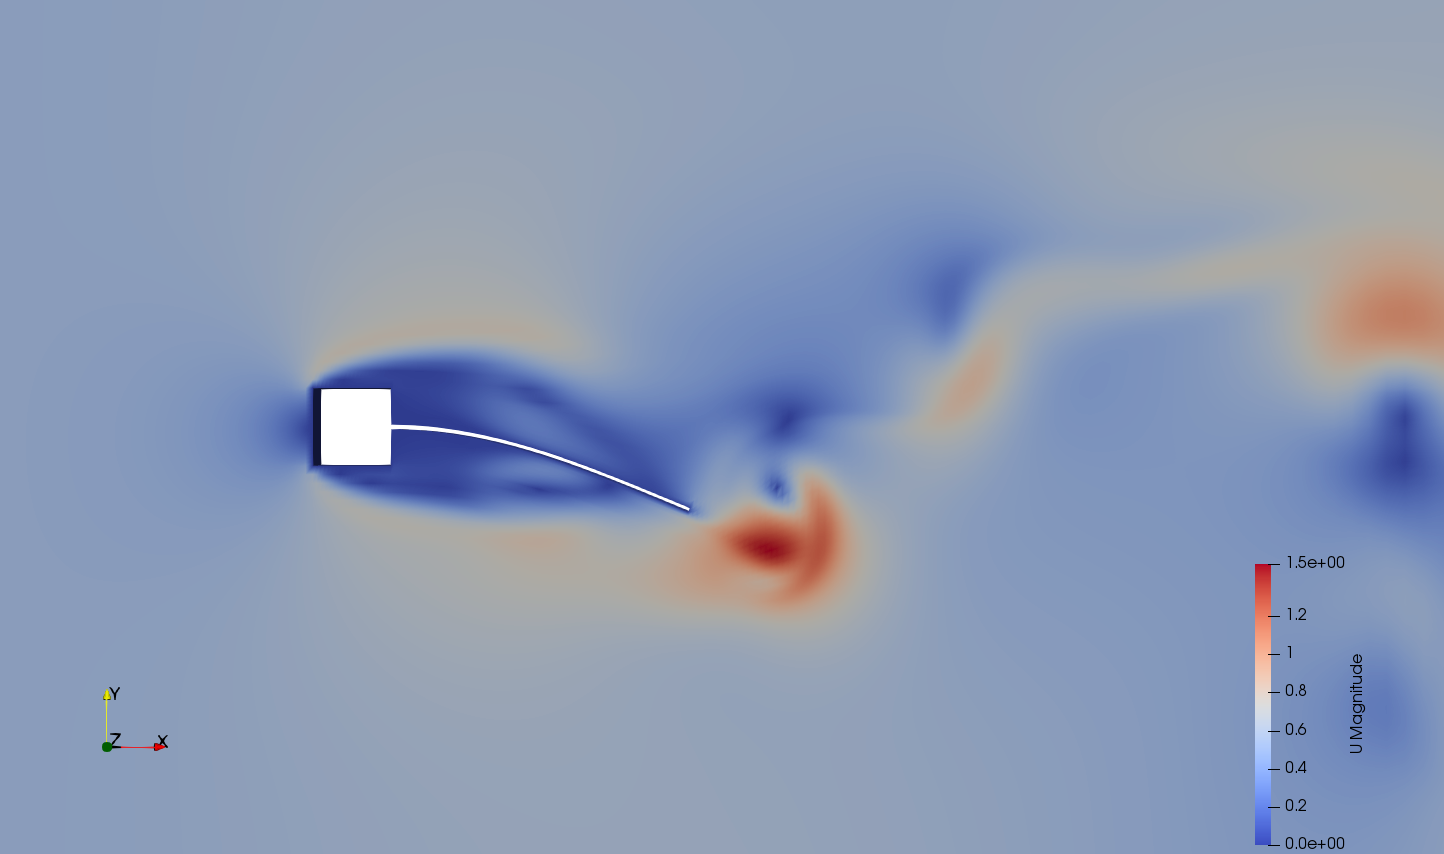
\includegraphics[width=\linewidth]{images/sq-cyl/sq_v1.png}
  \caption{t=3.37s velocity}
  \label{fig:sq_v1}
\end{subfigure}\hfil % <-- added
\begin{subfigure}{0.5\textwidth}
  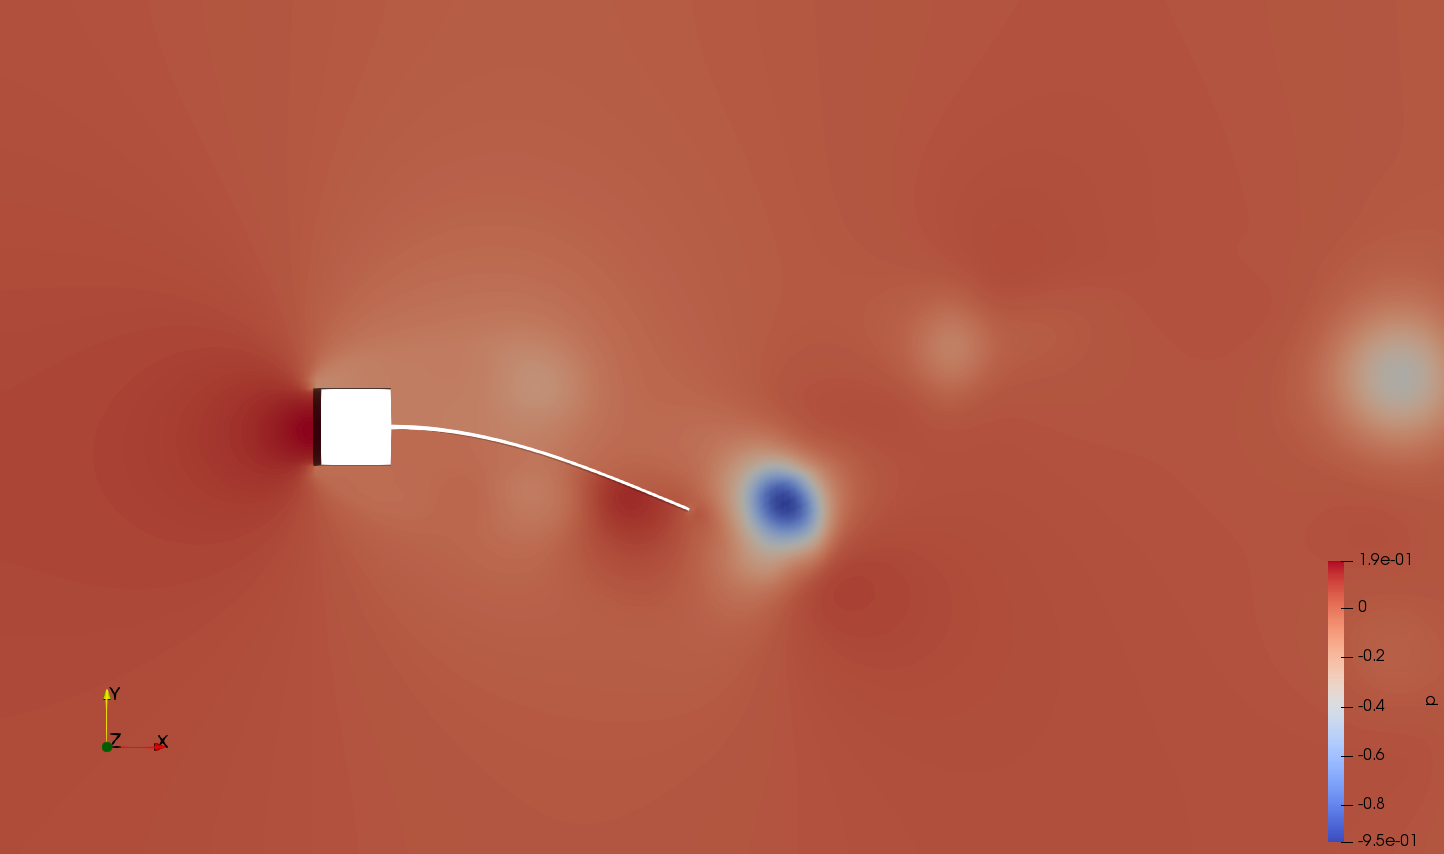
\includegraphics[width=\linewidth]{images/sq-cyl/sq_p1.png}
  \caption{t=3.37s pressure}
  \label{fig:sq_p1}
\end{subfigure}\hfil % <-- added

\medskip

\begin{subfigure}{0.5\textwidth}
  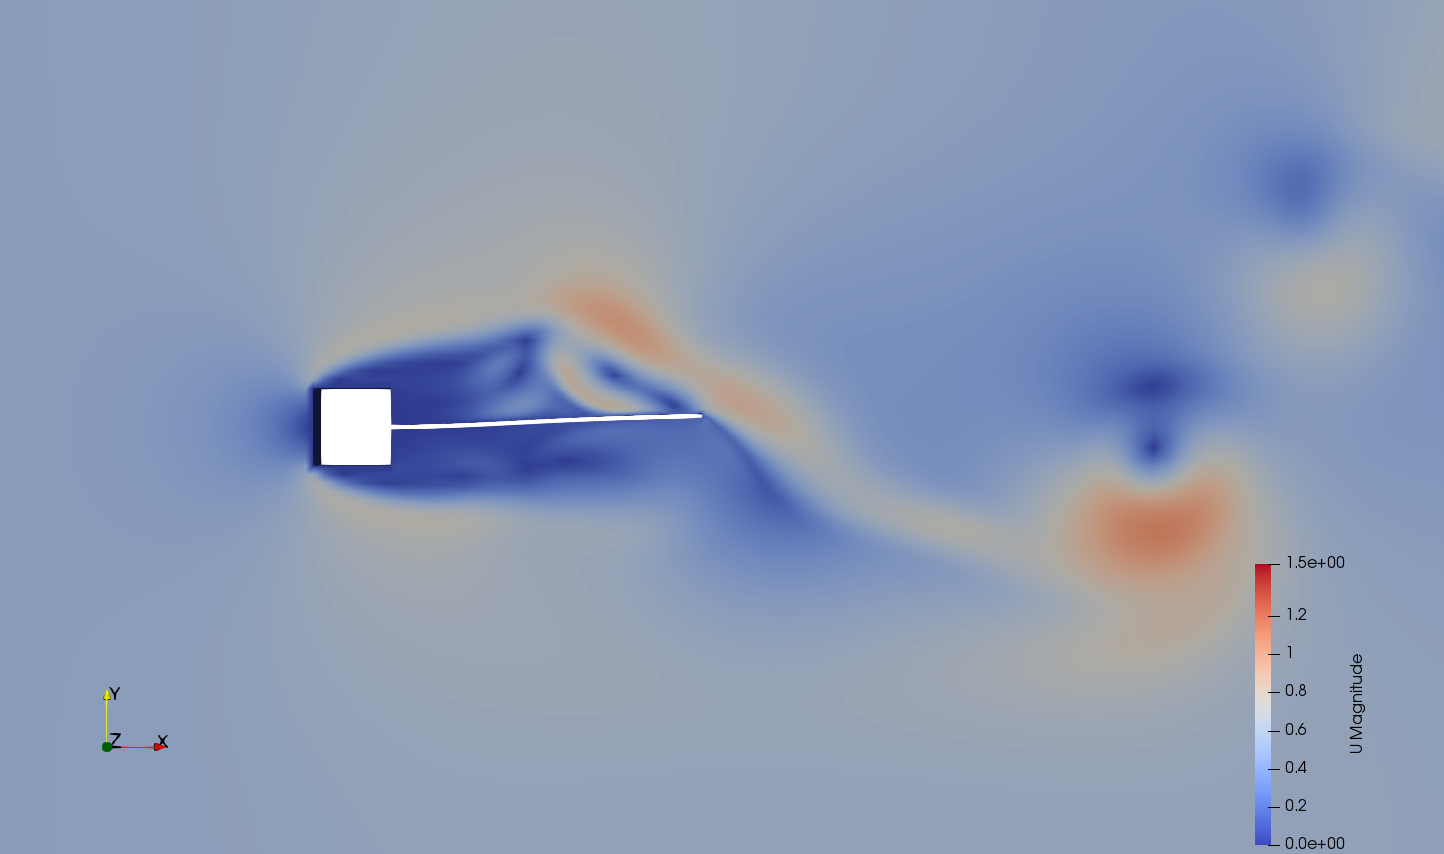
\includegraphics[width=\linewidth]{images/sq-cyl/sq_v2.png}
  \caption{t=3.47s velocity}
  \label{fig:sq_v2}
\end{subfigure}\hfil % <-- added
\begin{subfigure}{0.5\textwidth}
  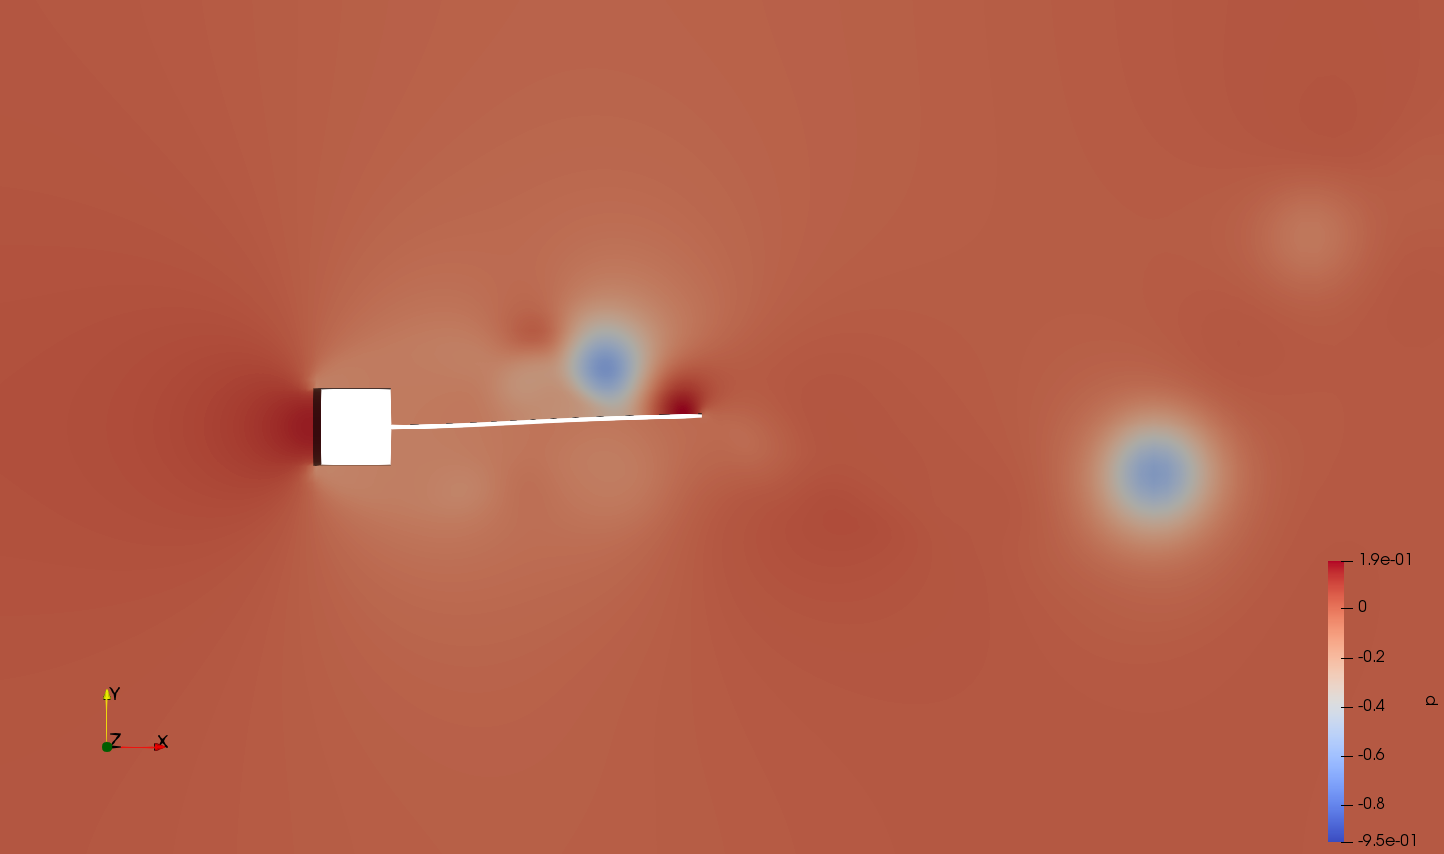
\includegraphics[width=\linewidth]{images/sq-cyl/sq_p2.png}
  \caption{t=3.47s pressure}
  \label{fig:sq_p2}
\end{subfigure}\hfil % <-- added

\medskip

\begin{subfigure}{0.5\textwidth}
  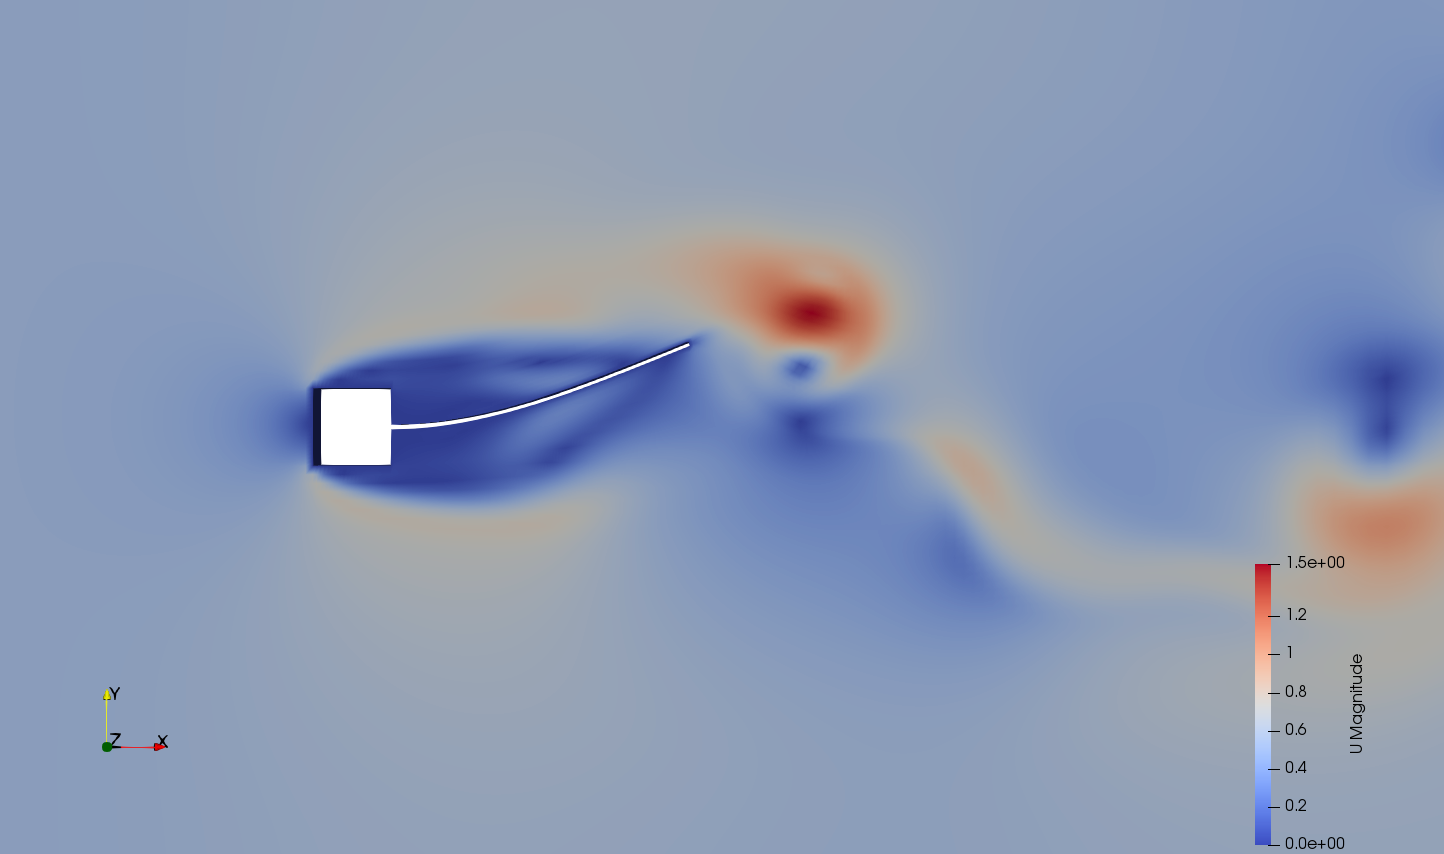
\includegraphics[width=\linewidth]{images/sq-cyl/sq_v3.png}
  \caption{t=3.53s velocity}
  \label{fig:sq_v3}
\end{subfigure}\hfil % <-- added
\begin{subfigure}{0.5\textwidth}
  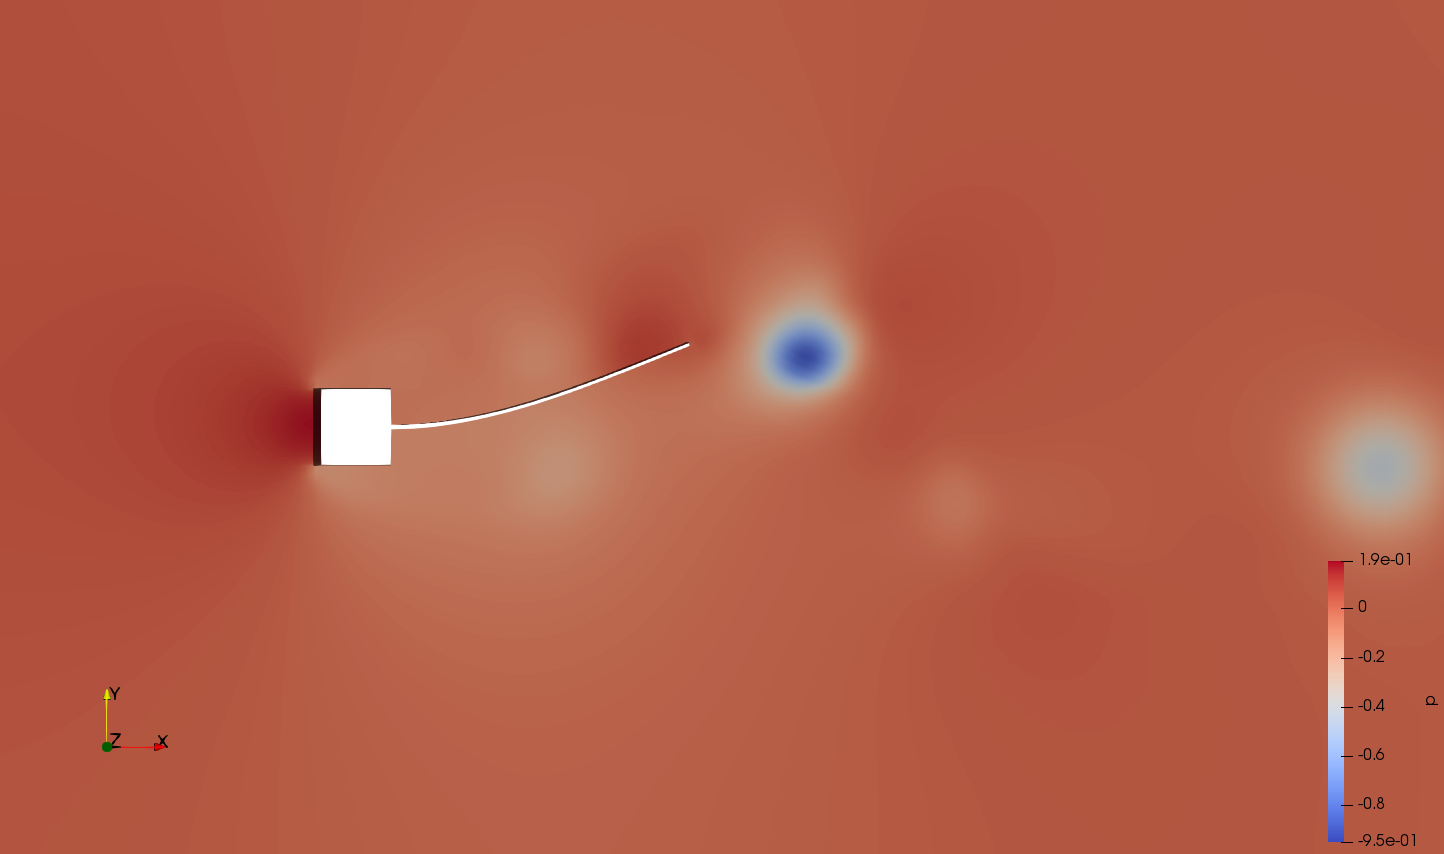
\includegraphics[width=\linewidth]{images/sq-cyl/sq_p3.png}
  \caption{t=3.53s pressure}
  \label{fig:sq_p3}
\end{subfigure}\hfil % <-- added

\caption{square bluff body: fluid solution}
\label{fig:sq_sol}
\end{figure}


Each time step converges with an average of 8 iterations, except for some situations where the coupling algorithm fails in making coupling forces converge. Those situations show a quite distorted fluid mesh that make the overall FSI problem harder to solve.

An higher average number of iterations agrees with the fact that a higher mass number, here in the order of $\mathcal{O} \left(10^{-2} \right) $, makes the problem strongly coupled.

\begin{figure}[htbp!]
	\centering
	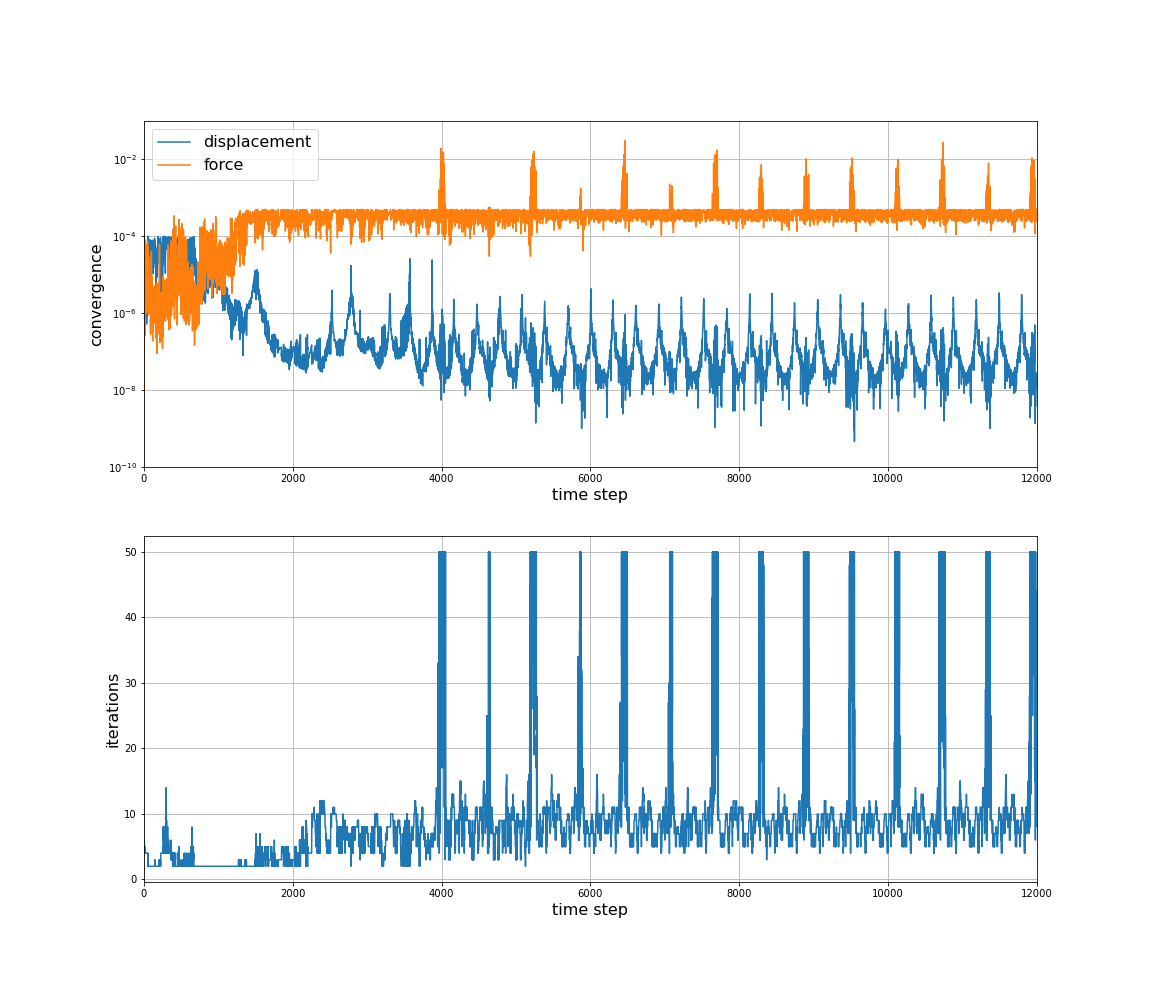
\includegraphics[width=0.95\textwidth, trim=0 80 0 100, clip]{images/sq-cyl/MBD_iterations_sq.png}
	\caption{square bluff body: convergence and iterations}
	\label{fig:sq_mbd_iter}
\end{figure}

As in the previous examples, the axial, shear and bending moment in each of the MBDyn elements are plotted in Figure \ref{fig:sq_mbd_internal}: in this case a temporal slice of $0.5s$ has been considered.

\begin{figure}[htbp!]
	\centering
	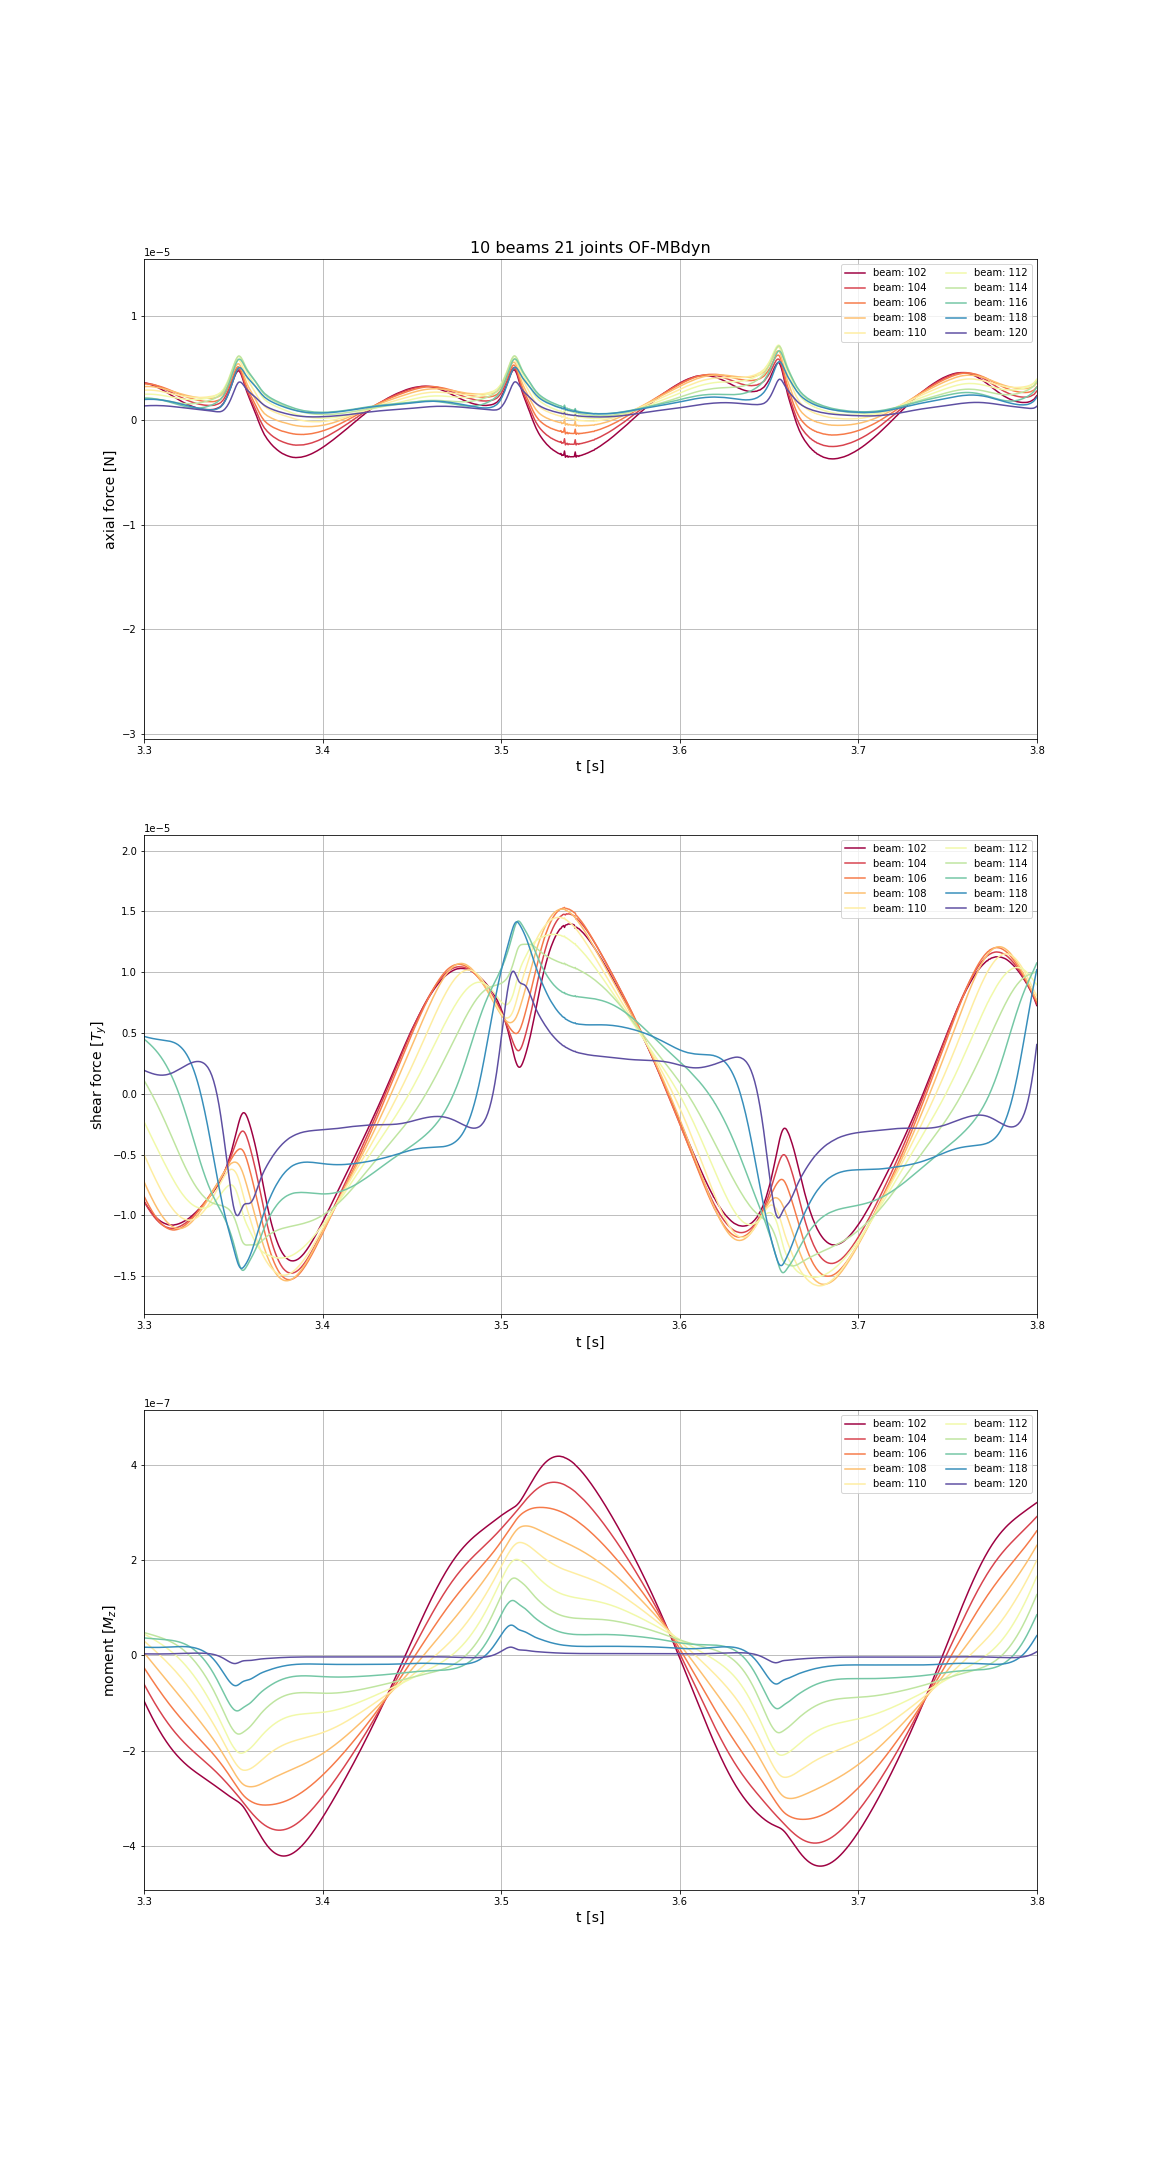
\includegraphics[width=0.92\textwidth, trim=0 230 0 230, clip]{images/sq-cyl/sq-flap_OF-MBDyn_act.png}
	\caption{square bluff body: MBDyn internal forces (detail)}
	\label{fig:sq_mbd_internal}
\end{figure}

\newpage

\subsection{Validation}

This problem has been used as a benchmark in a great number of studies in literature. The comparison between the studies is generally made on the tip displacement, in term of amplitude and frequency of oscillation. In Table \ref{table:sq-res} some results are given and compared to the present study.

\begin{table}[!ht]
	\begin{center}
		\begin{tabular}{ l | c  c } 
			Study & $f$ [\si{s^{-1}}] & $d_{y tip}$ [\si{mm}]   \\ 
			\hline
            Wall and Ramm \cite{ramm1998fluid} & $3.08$ & $13.1$ \\
            Kassiotis et al. \cite{kassiotis2011nonlinear} & $2.98$ & $10.5$ \\
            Wood et al. \cite{wood2010partitioned} & $2.94$ & $11.5$ \\
            Olivier et al. \cite{olivier2009fluid} & $3.17$ & $9.5$ \\
            Walhorn et al. \cite{walhorn2002space} & $3.14$ & $10.2$ \\
            Matthies and Steindorf \cite{matthies2003partitioned} & $3.13$ & $11.8$ \\ 
            Dettmer and Peric \cite{dettmer2006computational} & $3.03$ & $12.5$ \\
            Habchi et al. \cite{habchi2013partitioned} & $3.25$ & $10.2$ \\
            Froehle and Persson \cite{froehle2014high} & $3.18$ & $11.2$ \\
            Sanchez et al.\tablefootnote{Fluid Structure Interaction Problems using SU2. First SU2 Annual Developers Meeting. TU Delft, 6 September 2016}  & $3.15$ & $11.5$ \\
            \hline
            Present study    & $3.067$ & $11.2$ \\
            
		\end{tabular}
	\end{center}
	\caption{square bluff body: results}
	\label{table:sq-res}
\end{table}

The comparison shows a very good agreement among the studies: considering all the previous simulations, the average tip displacement is $11.2$ \si{mm} with a standard deviation of $1.06$ \si{mm} and the average frequency of oscillation is $3.1$ \si{Hz} with a standard deviation of $0.09$ \si{Hz}. 
This study, with a tip displacement of $11.2$ \si{mm} at a frequency of $3.067$ \si{Hz}, shows that the implementation of the adapter can give good results.

\newpage

\section{Turek-Hron FSI2 Benchmark}
\label{sec:FSI2}


Another well known benchmark concerning FSI simulations performed in incompressible flow regime is proposed by Turek and Hron \cite{turek2006proposal}.
A very important thing to notice about this study is that it is a proposal for a benchmark, as it is called  ``Proposal for numerical benchmarking of fluid-structure interaction between an elastic object and laminar incompressible flow''. So the paper gives a specific problem setup which others can contribute.

The fluid domain is similar to the one described in the previous chapter. The domain is again composed by a cylinder and a flap, but different flow velocities and structural properties are considered, so that 3 cases arise, commonly knonw as FSI1, FSI2 and FSI3.

For reasons that will be apparent in the next section, FSI2 is considered first. 

\subsection{Problem Description}

The structural part is composed of a round cylinder with a trailing thin flap, as described in Figure \ref{fig:fsi2_domain}. The geometrical data are given in Table \ref{table:fsi2-geom}.

\begin{table}[!htb]
	\begin{center}
		\begin{tabular}{ l c | r } 
			parameter & & value   \\ 
			\hline
			H  & [\si{m}] & $0.41$     \\
			L &  [\si{m}] & $2.5$  \\
			l  & [\si{m}] & $0.35$  \\
			h  & [\si{m}] & $0.02$  \\
			C  & [\si{m}] & $\left(0.2,0.2 \right)$  \\
			r  & [\si{m}] & $0.05$  \\
		\end{tabular}
	\end{center}
	\caption{FSI2: geometry}
	\label{table:fsi2-geom}
\end{table}

\begin{figure}[htbp!]
	\centering
	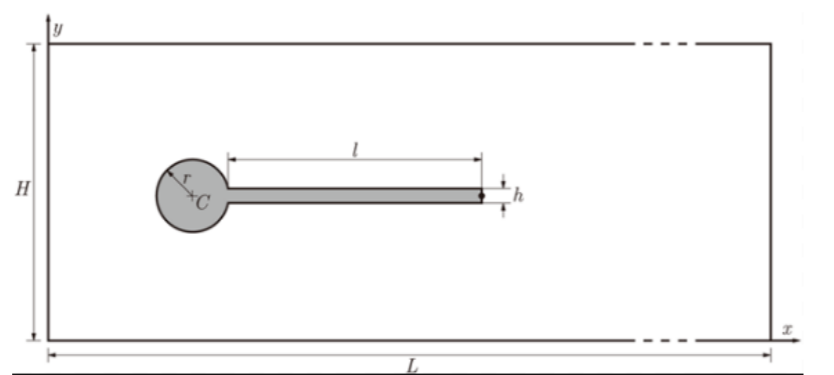
\includegraphics[width=0.92\textwidth, trim=0 0 50 0, clip]{images/FSI2/FSI2.png}
	\caption{FSI2: domain}
	\label{fig:fsi2_domain}
\end{figure}

\subsection{Fluid domain}

The fluid domain is represented in Figure \ref{fig:fsi2_domain} and has been simulated in OpenFOAM. The inlet is on the left with \textit{parabolic} flow velocity, the outlet is on the right, while all other boundaries are \textit{no-slip} walls.

The fluid domain is discretized in an structured hexaedral mesh as depicted in Figure \ref{fig:FSI2_mesh}. The main fluid and mesh values are given in Table \ref{table:FSI2-fluid} and \ref{table:FSI2-mesh}. 

\begin{figure}[htbp!]
	\centering
	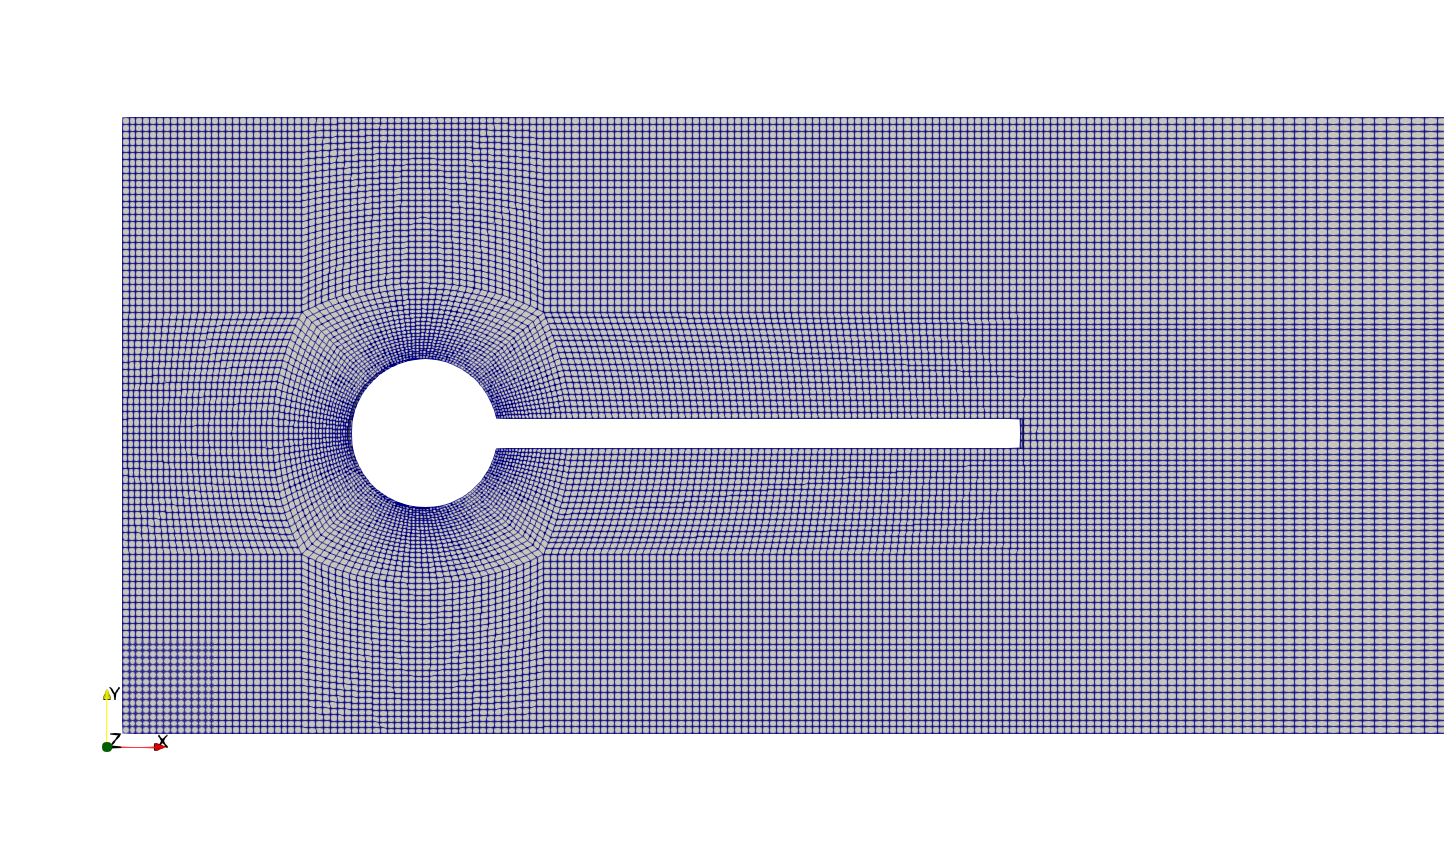
\includegraphics[width=0.9\textwidth]{images/FSI2/FSI2-mesh.png}
	\caption{FSI2: fluid mesh}
	\label{fig:FSI2_mesh}
\end{figure}


\begin{table}[!htb]
	\begin{center}
		\begin{tabular}{ l c l | c } 
			parameter & & & value  \\ 
			\hline
			fluid density  & $\rho$ & \si{kg.m^{-3}} & $1000$   \\
			kinematic viscosity & $\nu$& \si{m^{2}.s^{-1}} & $1 \cdot 10^{-3}$  \\
%			Reynolds length & $l_{Re}$ & $0.1$ & \si{m} \\
			Reynolds number & Re &  & $100$ \\
			max flow velocity & $\vec{u}_{max}$ & \si{m.s^{-1}} & $1.5$ \\
			mean flow velocity & $\vec{u}$ & \si{m.s^{-1}} & $1$ \\
			flow type & & & laminar \\
		\end{tabular}
	\end{center}
	\caption{FSI2: fluid properties}
	\label{table:FSI2-fluid}
\end{table}



\begin{table}[!htb]
	\begin{center}
		\begin{tabular}{ l c | c } 
			parameter & & value   \\ 
			\hline
			number of mesh points  & $n_{dof}$ & 51464     \\
			number of cells & $n_c$ & 25224  \\
			number of interface cells  & $n_{int}$ & 180  \\			
		\end{tabular}
	\end{center}
	\caption{FSI2: mesh properties}
	\label{table:FSI2-mesh}
\end{table}


\subsection{Solid domain}

The properties of the solid are reported in Table \ref{table:FSI2-solid}.

\begin{table}[!htb]
	\begin{center}
		\begin{tabular}{ l c  l | c } 
			parameter & & value &    \\ 
			\hline
			solid density  & $\rho$ & \si{kg.m^{-3}} & $10000$    \\
			Elastic modulus  & E & \si{Pa} & $1.4\cdot 10^6$    \\
			Poisson coefficient & $\nu$ & & $0.4$  \\
			%			Reynolds length & $l_{Re}$ & $0.1$ & \si{m} \\
			%			Reynolds number & Re & $\approx 1000$ & \\
		\end{tabular}
	\end{center}
	\caption{FSI2: solid properties}
	\label{table:FSI2-solid}
\end{table}

The MBDyn model is the same as the one used in \ref{sec:sq-cyl-bench} and is composed of 10 \texttt{beam3} elements, with a structural damping of $1\cdot10^{-2}$.

The interface mesh is divided into 90 faces and is shown in Figure \ref{fig:FSI2_struct_mesh}. 

\begin{figure}[htbp!]
	\centering
	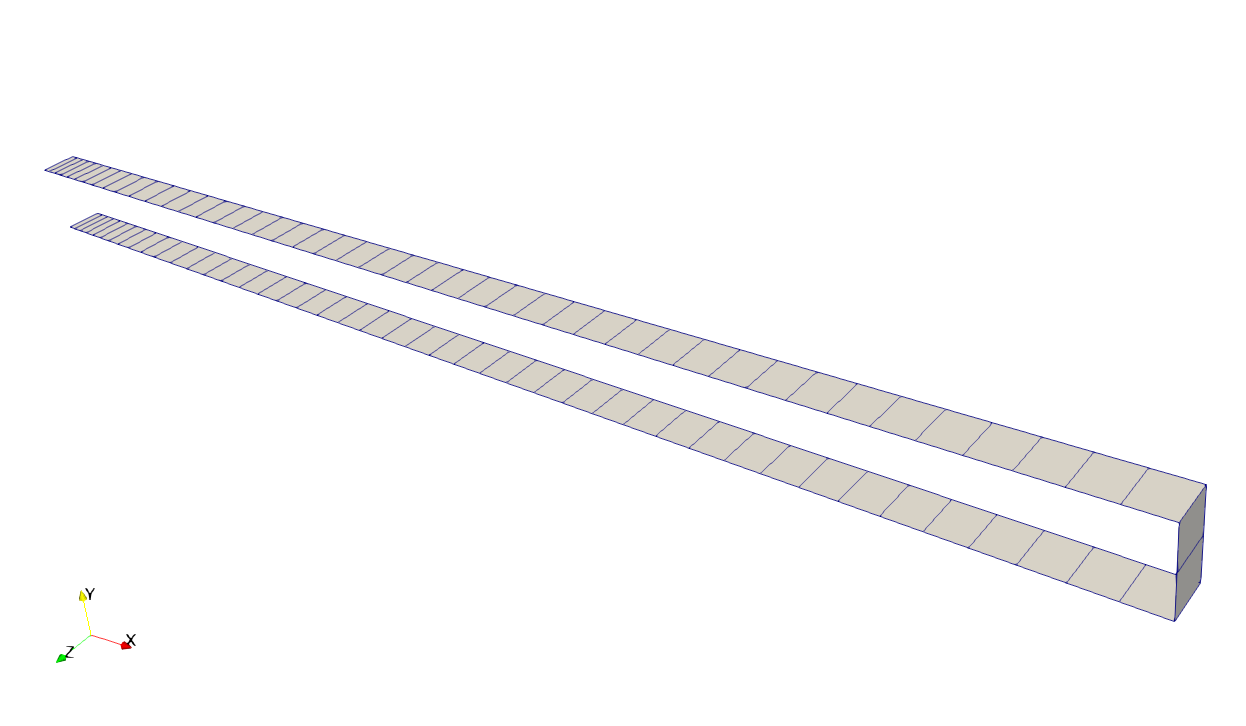
\includegraphics[width=0.9\textwidth, trim=0 50 0 150, clip]{images/FSI2/fsi2_struct_mesh.png}
	\caption{FSI2: structural interface mesh}
	\label{fig:FSI2_struct_mesh}
\end{figure}


\subsection{Coupling parameters}


The main coupling data are given in Table \ref{table:FSI2-coupling}. In this case a time step of $1ms$ is enough for the simulation.

\begin{table}[!htb]
	\begin{center}
		\begin{tabular}{ l c  l| c } 
			parameter & & & value   \\ 
			\hline
			simulation time  & $t$& \si{s} & 15      \\
			step size & $\Delta t$ & \si{s} & $1 \cdot 10^{-3}$   \\
			\hline
			coupling scheme & & & serial implicit  $S\rightarrow F$  \\
			coupling algorithm & & &  IQN-ILS  \\
			displacement rel. convergence limit & & & $10^{-4}$ \\
			force rel. convergence limit &&  & $2 \cdot 10^{-4}$  \\
      		interface mesh mapping & & & RBF  \\
			
		\end{tabular}
	\end{center}
	\caption{FSI2: coupling parameters}
	\label{table:FSI2-coupling}
\end{table}


\subsection{Results}

The problem considered is characterized by the adimensional parameters given in Table \ref{table:FSI2-adim} and its solution is represented in Figure \ref{fig:FSI2_sol}.

\begin{table}[!htb]
	\begin{center}
		\begin{tabular}{ l c | c } 
			parameter & & value   \\ 
			\hline
			mass number  & $M$ & $0.1$     \\
			reduced velocity & $U_R$ & $ 8.45\cdot 10^{-2}$  \\
			Cauchy number  & $C_Y$ & $  7.14 \cdot 10^{-4}$  \\			
		\end{tabular}
	\end{center}
	\caption{FSI2: adimensional numbers}
	\label{table:FSI2-adim}
\end{table}

In this case, the ramp applied to fluid forces at the beginning of the simulation is longer in order to make the fluid and structure settle: during the first $500$ \si{ms} forces are scaled to $10\%$ and reach $100\%$ after another $500$ \si{ms}.

Alternating vortices begin developing and the flap begins oscillating with an increasing amplitude. After around 4 seconds reaches a vortex lock-in regime, as shown in Figure \ref{fig:FSI2_displacement} (in particular the tip displacement in \textit{y} direction).


\begin{figure}[htbp!]
	\centering
	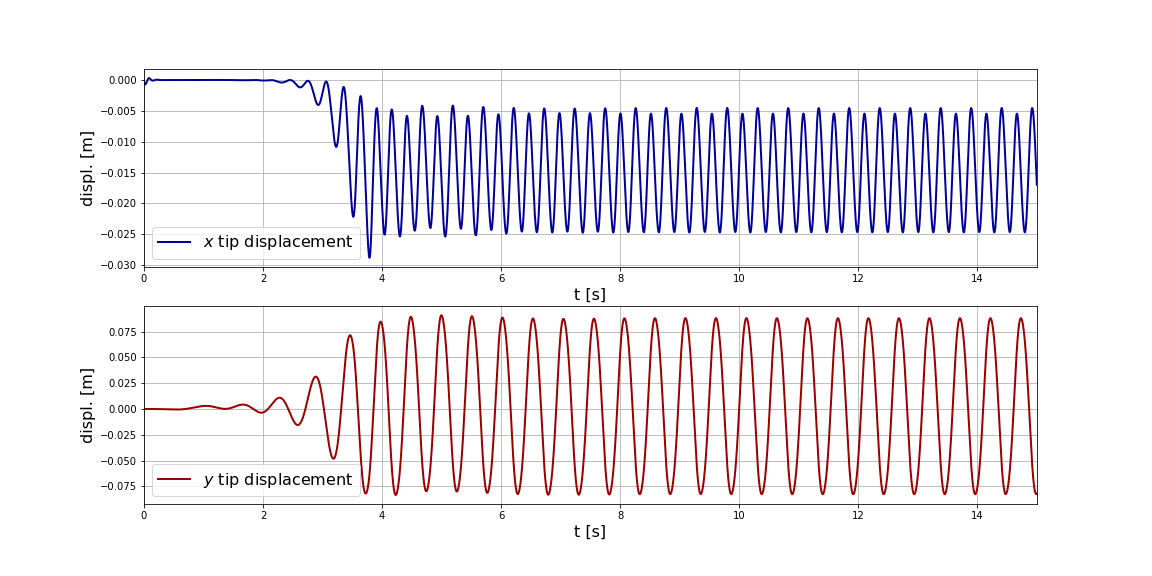
\includegraphics[width=0.98\textwidth, trim=20 20 50 50, clip]{images/FSI2/disp_fsi2.png}
	\caption{FSI2: tip displacement}
	\label{fig:FSI2_displacement}
\end{figure}

Forces are measured on the whole structure on the fluid side, while are measured on the flap in the solid domain. Figure \ref{fig:FSI2_force} shows a detail of $2$ \si{s} of simulation. The difference in \textit{x}-direction represents the drag force on the cylinder.
\begin{figure}[htbp!]
	\centering
	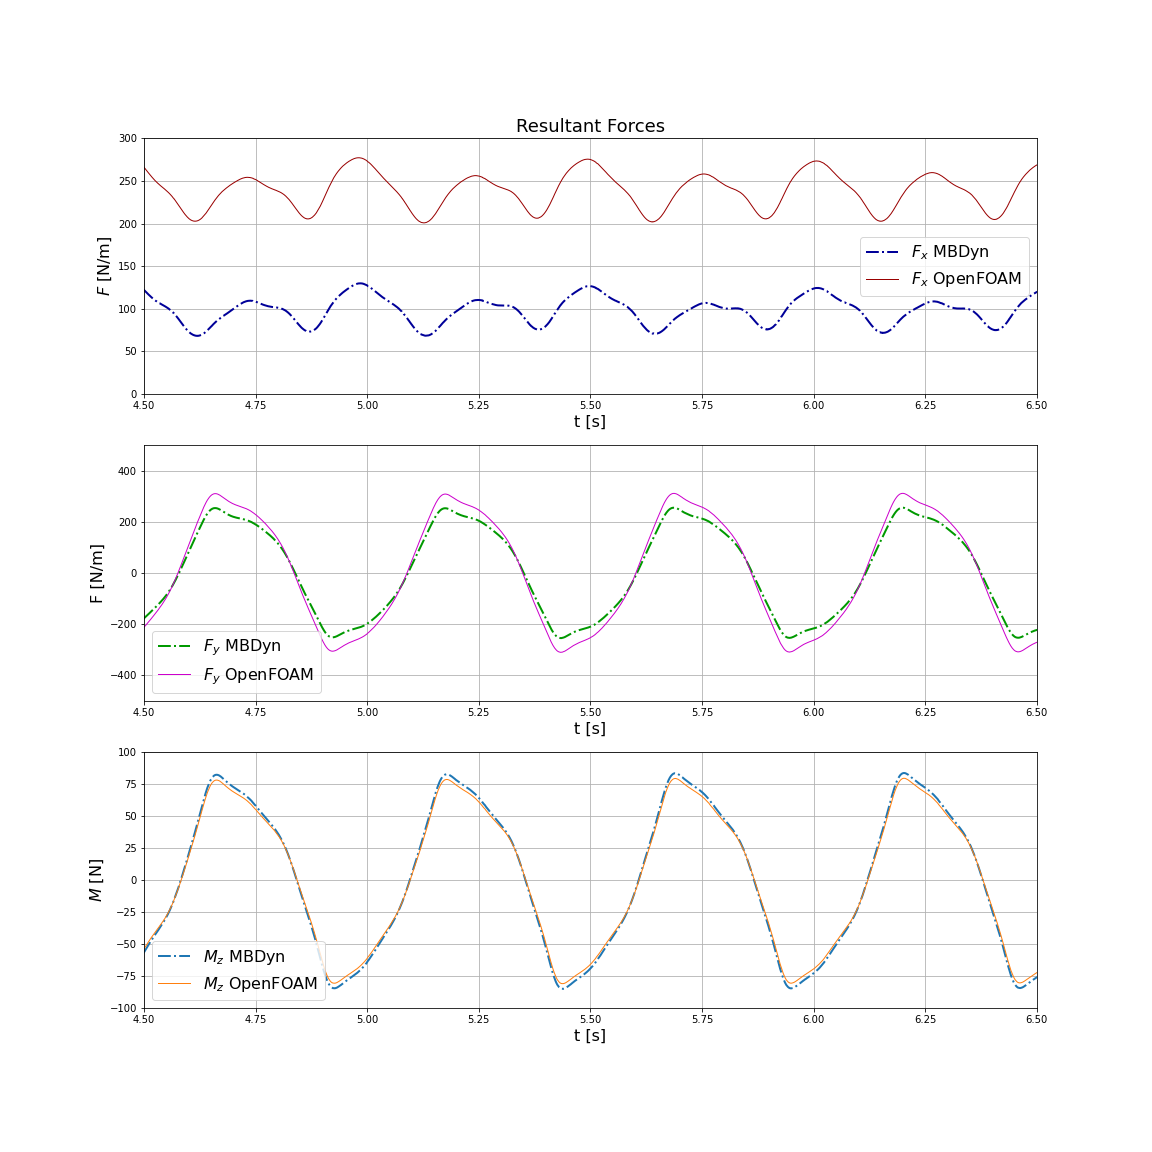
\includegraphics[width=0.98\textwidth, trim=20 100 20 100, clip]{images/FSI2/forces_fsi2.png}
	\caption{FSI2: resultant forces (detail)}
	\label{fig:FSI2_force}
\end{figure}


\begin{figure}[htb]
\centering % <-- added
\begin{subfigure}{0.5\textwidth}
  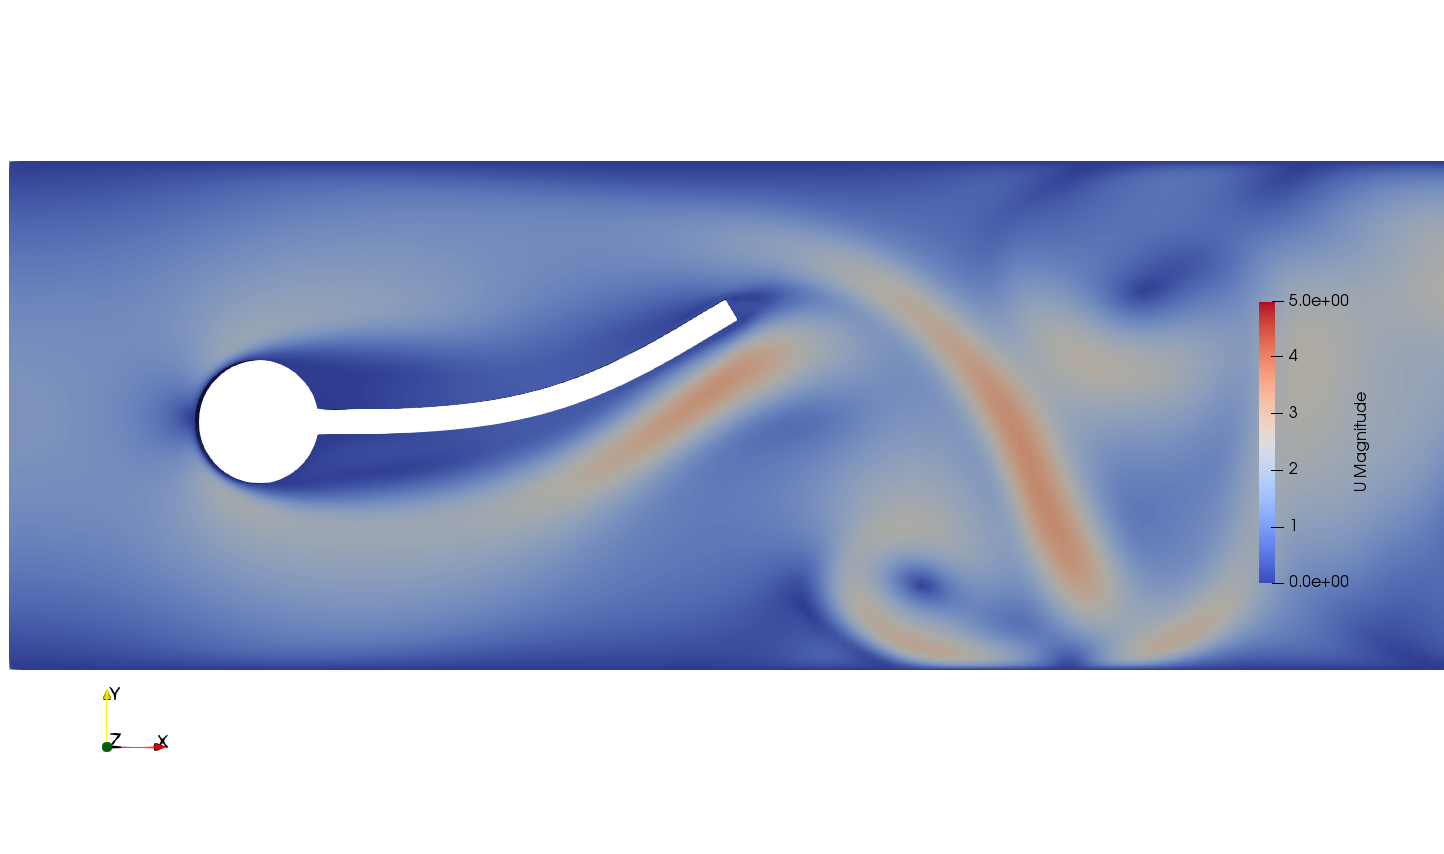
\includegraphics[width=\linewidth, trim=0 120 0 120, clip]{images/FSI2/fsi2_v1.png}
  \caption{t=5.0s velocity}
  \label{fig:fsi2_v1}
\end{subfigure}\hfil % <-- added
\begin{subfigure}{0.5\textwidth}
  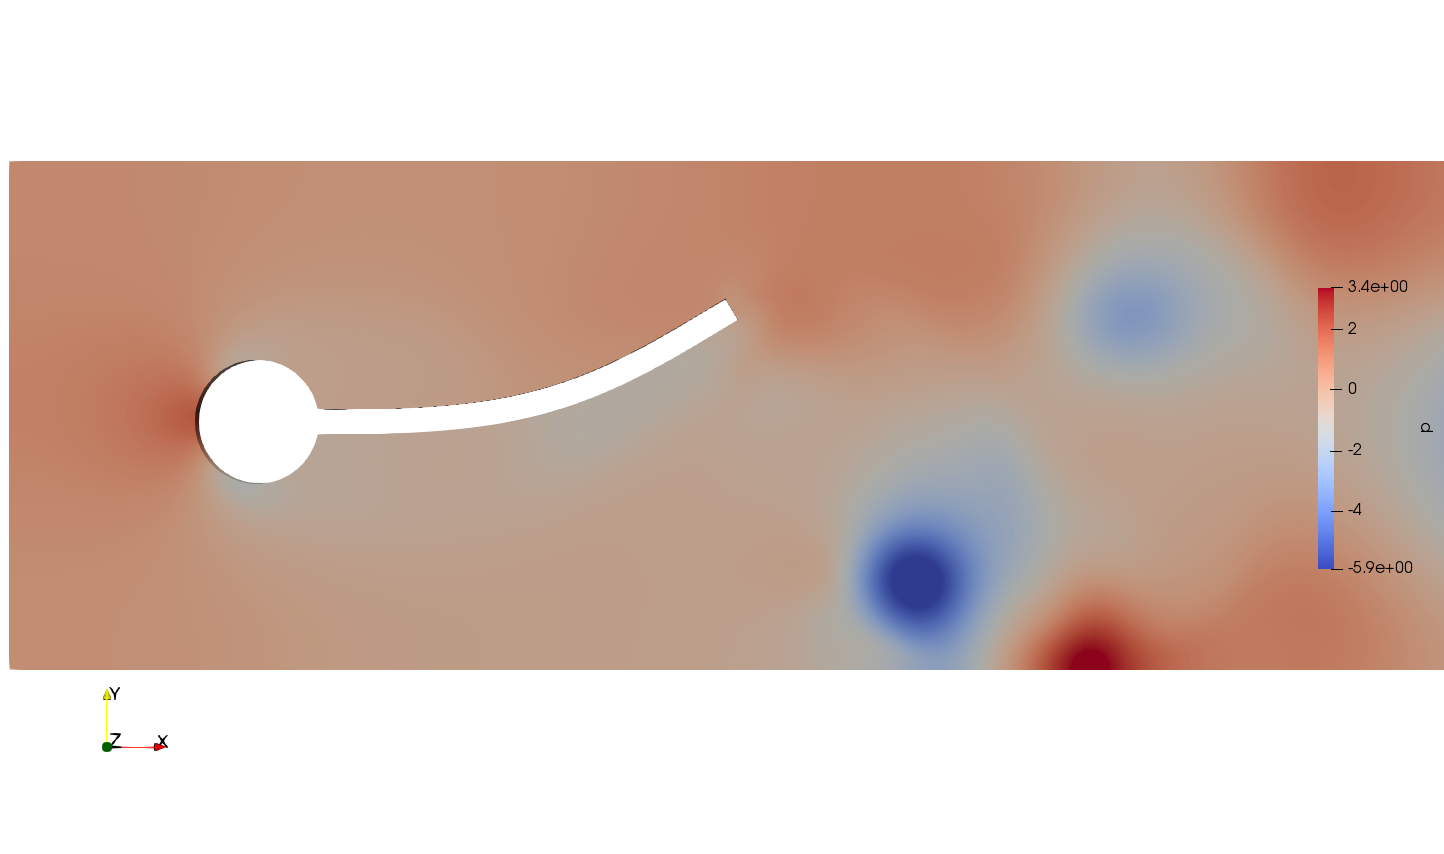
\includegraphics[width=\linewidth, trim=0 120 0 120, clip]{images/FSI2/fsi2_p1.png}
  \caption{t=5.0s pressure}
  \label{fig:fsi2_p1}
\end{subfigure}\hfil % <-- added

\medskip

\begin{subfigure}{0.5\textwidth}
  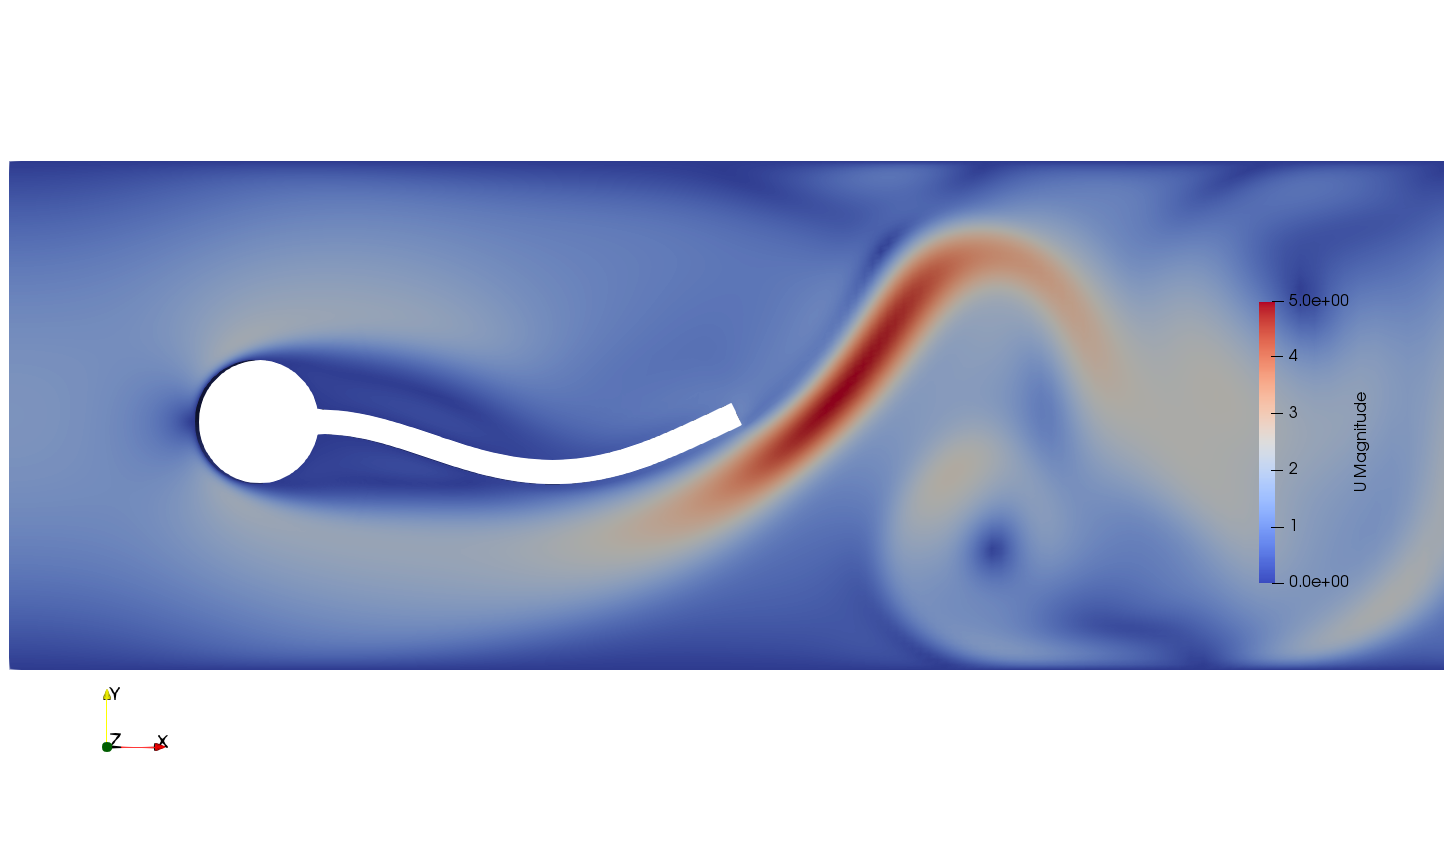
\includegraphics[width=\linewidth, trim=0 120 0 120, clip]{images/FSI2/fsi2_v2.png}
  \caption{t=5.135s velocity}
  \label{fig:fsi2_v2}
\end{subfigure}\hfil % <-- added
\begin{subfigure}{0.5\textwidth}
  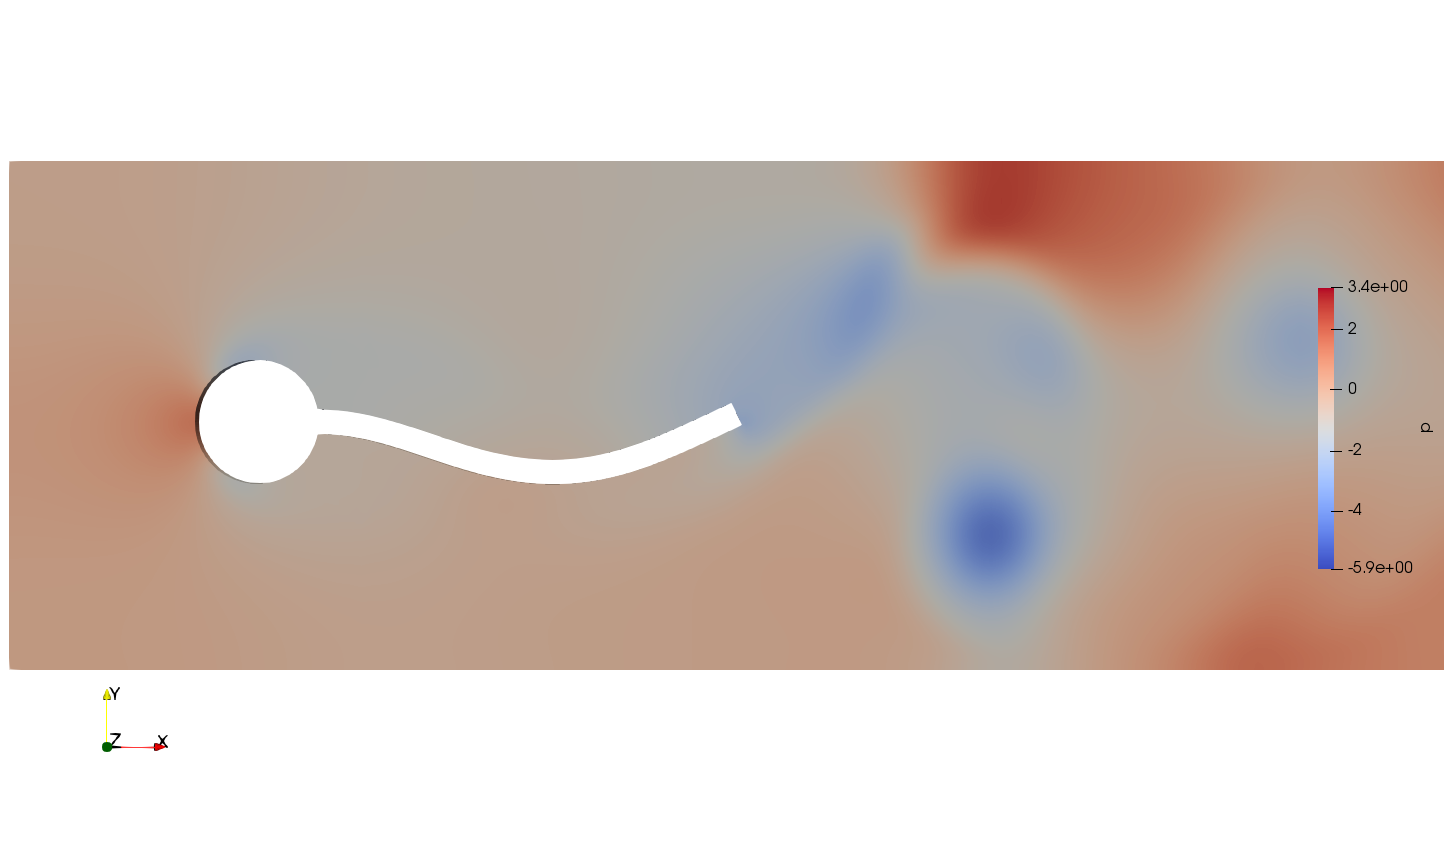
\includegraphics[width=\linewidth, trim=0 120 0 120, clip]{images/FSI2/fsi2_p2.png}
  \caption{t=5.135s pressure}
  \label{fig:fsi2_p2}
\end{subfigure}\hfil % <-- added

\medskip

\begin{subfigure}{0.5\textwidth}
  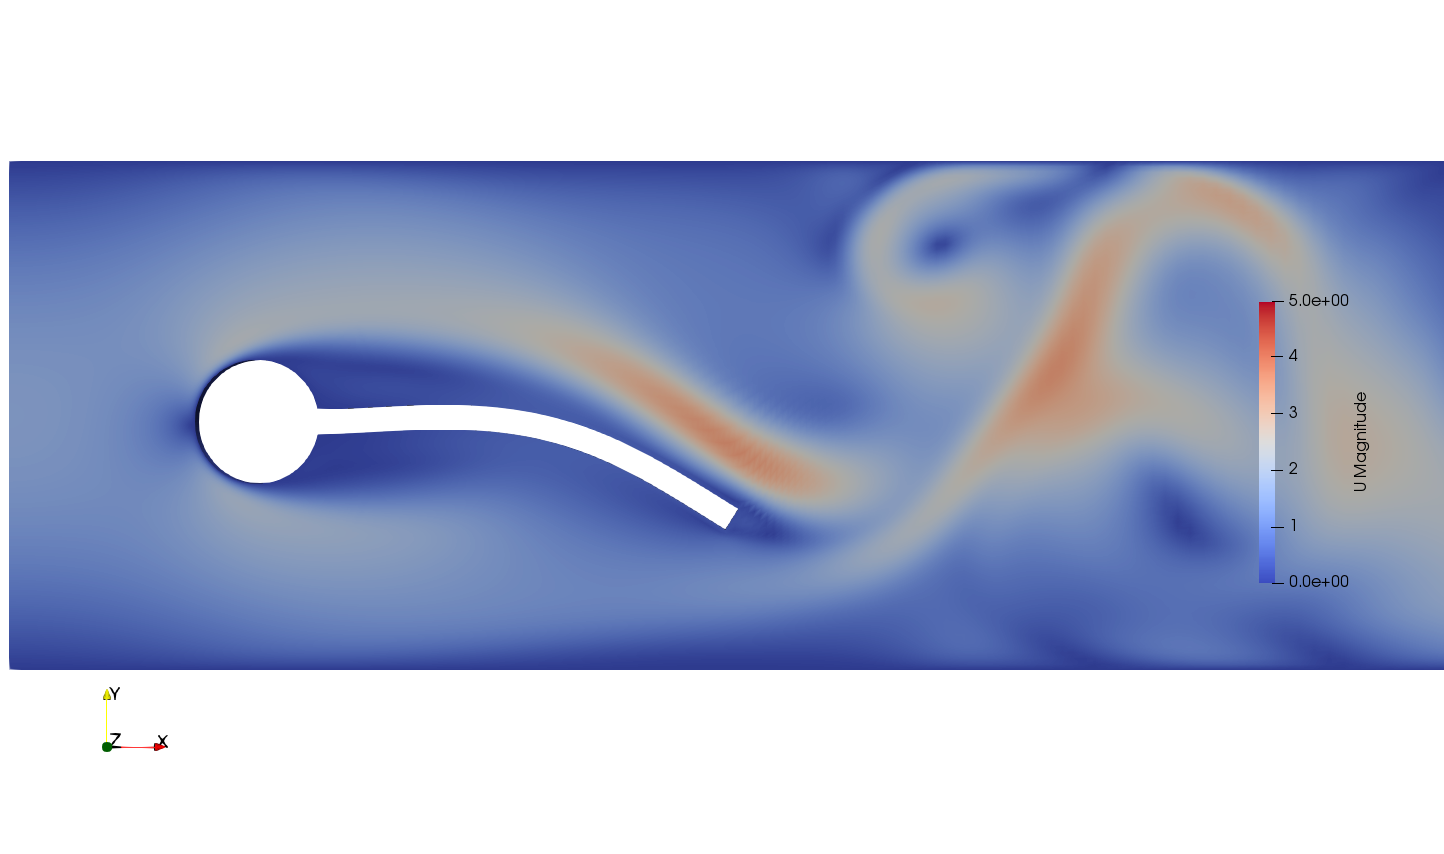
\includegraphics[width=\linewidth, trim=0 120 0 120, clip]{images/FSI2/fsi2_v3.png}
  \caption{t=5.27s velocity}
  \label{fig:fsi2_v3}
\end{subfigure}\hfil % <-- added
\begin{subfigure}{0.5\textwidth}
  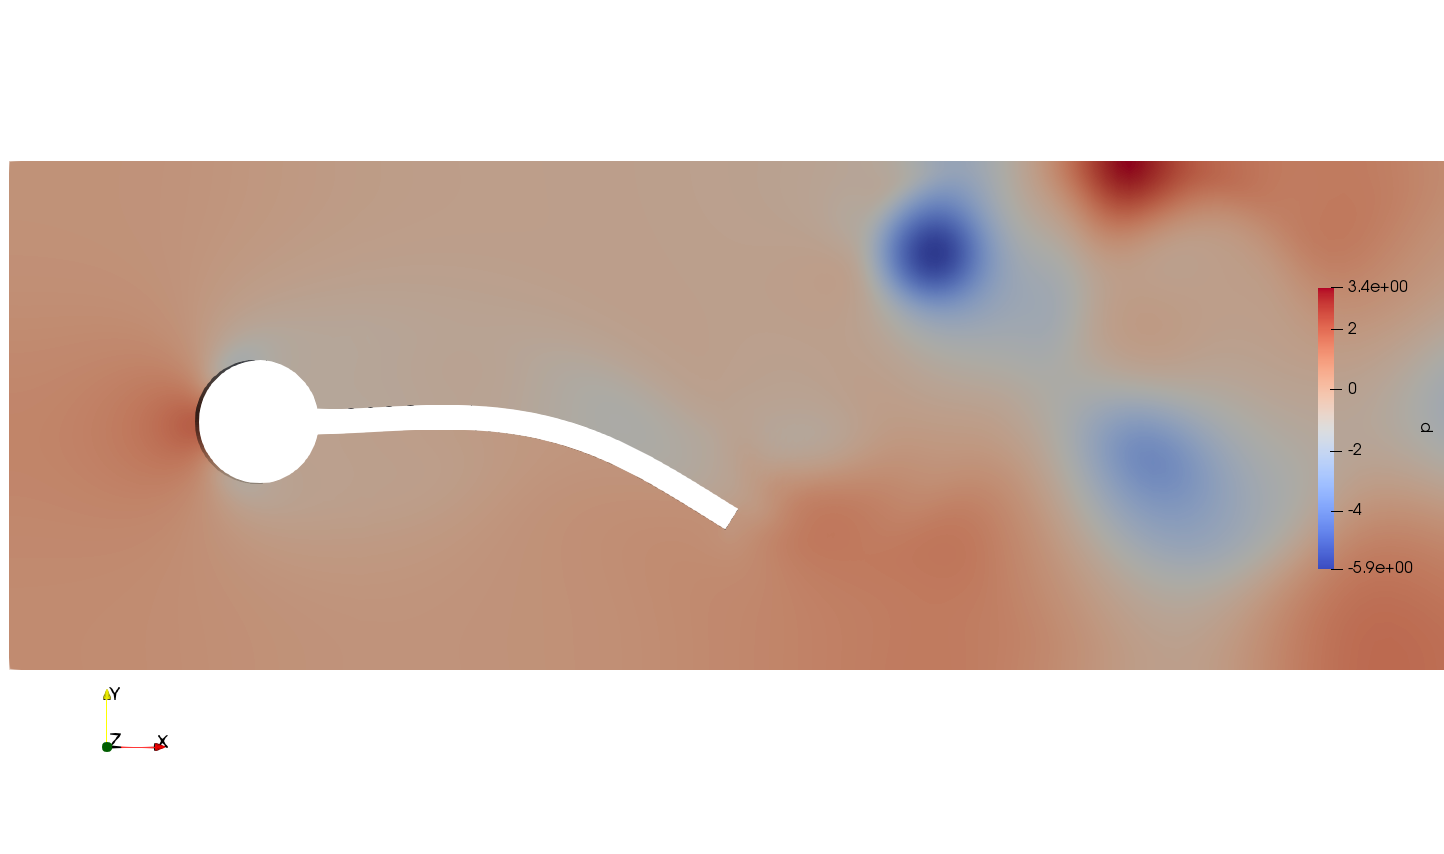
\includegraphics[width=\linewidth, trim=0 120 0 120, clip]{images/FSI2/fsi2_p3.png}
  \caption{t=5.27s pressure}
  \label{fig:fsi2_p3}
\end{subfigure}\hfil % <-- added

\caption{FSI2: fluid solution}
\label{fig:FSI2_sol}
\end{figure}


Each time step converges with an average of 14.5 iterations, which again confirms the trend of more coupling iterations as the mass number increases.

\begin{figure}[htbp!]
	\centering
	\includegraphics[width=0.95\textwidth, trim=0 80 0 100, clip]{images/FSI2/MBD_iterations_fsi2.png}
	\caption{FSI2: convergence and iterations}
	\label{fig:FSI2_mbd_iter}
\end{figure}

As in the previous examples, the axial, shear and bending moment in each of the MBDyn elements are plotted in Figure \ref{fig:sq_mbd_internal}: in this case a temporal slice of $25s$ has been considered. The values plotted here consider a beam with $2mm$ width: i.e. the thickness of the solid and fluid domains considered in this case.

\begin{figure}[htbp!]
	\centering
	\includegraphics[width=0.92\textwidth, trim=0 230 0 230, clip]{images/FSI2/FSI2_OF-MBDyn_act.png}
	\caption{FSI2: MBDyn internal forces (detail)}
	\label{fig:FSI2_mbd_internal}
\end{figure}


\subsection{Validation}

Turek and Hron benchmarks have been used as a benchmark in many studies considering strongly coupled FSI simulations. 

FSI2 is fully oscillating while the same problem, considering the structure rigid (named CFD2 in \cite{turek2006proposal}) is steady: for this reason it is considered an excellent check for interaction mechanisms \cite{turek2010numerical}.

Besides, FSI2 gives the largest deformation and in some cases it is considered the most difficult of the three benchmarks \cite{richter2015time}, as it gives deformations 2.5 times greater than the flap height.

The comparison of the results can be done in terms of tip displacement and in terms of lift and drag force applied to the whole structure. The results given in the original paper and in a review made by the same authors, together with other studies found in literature are compared to the present study in Table \ref{table:FSI2-results-d} for the data concerning tip displacement, and in Table \ref{table:FSI2-results-f} for the forces applied to the structure.


\begin{table}[!htb]
	\begin{center}
		\begin{tabular}{ l | c c | c c  |  } 
			Study & $d_{x tip}$ [\si{mm}] & f [\si{Hz}] & $d_{y tip}$ [\si{mm}] & f [\si{Hz}] \\ 
			\hline
			\hline
			Benchmark  \cite{turek2006proposal} & $-14.58\pm12.44$ & $3.8$ & $1.23\pm80.6$ & $2.0$     \\
			Turek et al. (2010) \cite{turek2010numerical} & $-14.85\pm12.70$ & $3.86$ & $1.30\pm81.7$ & $1.93$ \\
			Gjertsen \cite{gjertsen2017development} & $-14.83\pm13.11$ & & $1.24\pm81.6$ & \\
			Degroote \cite{degroote2009interface}  & $-14.07\pm12.37$ & $3.7$ & $1.18\pm76.5$ & $1.9$ \\
			\hline
			Present study & $-14.95\pm9.85$ & $3.87$ & $2.78\pm83.39$ & $1.93$ \\ 
		\end{tabular}
	\end{center}
	\caption{FSI2: comparison of results (displacements)}
	\label{table:FSI2-results-d}
\end{table}

\begin{table}[!htb]
	\begin{center}
		\begin{tabular}{ l | c c | c c  |  } 
			Study & drag [\si{N.m^{-1}}] & f [\si{Hz}] & lift [\si{N.m^{-1}}] & f [\si{Hz}]    \\ 
			\hline
			\hline
			Benchmark  \cite{turek2006proposal} & $208.83\pm73.75$ & $3.8$ & $0.88\pm234.2$ & $2.0$     \\
			Turek et al. (2010) \cite{turek2010numerical} & $215.06\pm77.63$ & $3.86$ & $0.61\pm237.8$ & $1.93$\\   
			Gjertsen \cite{gjertsen2017development} & $161.50\pm73.75$ & & $0.88\pm234.2$ & \\
			Degroote \cite{degroote2009interface}  & $217.52\pm84.65$ & $3.7$ & $-0.74\pm267.6$ & $1.9$ \\
			\hline
			Present study & $239.13\pm31.93$ & $3.87$ & $3.43\pm308.57$ & $1.93$ \\
		\end{tabular}
	\end{center}
	\caption{FSI2: comparison of results (forces)}
	\label{table:FSI2-results-f}
\end{table}


The study \cite{turek2010numerical} gives 7 different methods and results for FSI1 and FSI3 test cases. In the numerical results it is stated that ``clear differences between the different approaches with regard to accuracy are visible. Particularly for the drag and lift values, which lead to differences of up to order $50\%$, and also for the displacement values which are in the range of $10\%$ errors''.

For the FSI2 test case only the results from the initial Hron and Turek paper \cite{turek2006proposal} and a few others are available.

Comparing the results, with previous studies (Table \ref{table:FSI2-results-d}), mean displacement in x direction is very close to all other results (mainly due to mean pressure applied to the tip face), while mean oscillation is lower of about $3mm$. The displacement in y direction is about $2mm$ higher. It looks like the MBDyn structure is a bit more flexible (as also seen in Section \ref{sec:cx-mbd} for the vertical flap). This also reflects the fact that average drag and lift are higher.

The greatest difference can be seen in the oscillation of drag, which is much smaller than other studies. The data collected during the simulation allow to separate the contribution of the cylinder from the one of the flap (see first graph of Figure \ref{fig:FSI2_force}). The cylinder has an average drag of $140$ \si{N.m^{-1}} with a standard deviation of $\approx7$ \si{N.m^{-1}}. Considering that the average $C_D$ of a cylinder at $Re=100$ is around $1.35$ \cite{qin2017direct}, and an average fluid velocity around the cylinder of about $1.4$ \si{m.s^{-1}}, the contribution is as expected. The contribution of the flap seems to be much lower than expected.

As previously stated, the results for the FSI3 case differ by in some cases $50\%$ for Drag and Lift. With this in mind, in the FSI2 case it is reasonable to assume that since there were such differences in the results for different implementations for the FSI3 results, we would expect similar behavior in the FSI2 results.


\newpage


\section{Turek-Hron FSI3 Benchmark}
\label{sec:FSI1-FSI3}

Omitting for a while the test case named FSI1 as it is not oscillating, the other benchmark proposed in \cite{turek2006proposal}, named FSI3, is very similar to FSI2 with the only different properties shown in Table \ref{table:FSI3-diff}. The corresponding adimensional numbers are given in Table \ref{table:FSI3-adim}. 



\begin{table}[!htb]
	\begin{center}
		\begin{tabular}{ l c l | c | c } 
			parameter & & & FSI2 & FSI3   \\ 
			\hline
			solid density  &  $\rho$ & \si{kg.m^{-3}} & $10000$ & $1000$     \\
			Elastic modulus  & E & \si{Pa} & $1.4\cdot 10^6$ & $5.6\cdot 10^6$   \\
			max flow velocity & $\vec{u}_{max}$ & \si{m.s^{-1}} & $1.5$ & $3$ \\
			mean flow velocity & $\vec{u}$ & \si{m.s^{-1}} & $1$ & $2$  \\
		\end{tabular}
	\end{center}
	\caption{FSI2-FSI3: different parameters}
	\label{table:FSI3-diff}
\end{table}


\begin{table}[!htb]
	\begin{center}
		\begin{tabular}{ l c | c | c} 
			parameter & & FSI2 & FSI3   \\ 
			\hline
			mass number  & $M$ & $0.1$ & $1$     \\
			reduced velocity & $U_R$ &  $8.45 \cdot 10^{-2}$  & $2.67\cdot 10^{-2}$  \\
			Cauchy number  & $C_Y$ & \cellcolor{yellow!25}  $7.14\cdot 10^{-4}$  & \cellcolor{yellow!25} $7.14\cdot 10^{-4}$  \\
			Reynolds number & $Re$ & $100$ & $200$ \\	
		\end{tabular}
	\end{center}
	\caption{FSI2-FSI3: adimensional numbers}
	\label{table:FSI3-adim}
\end{table}


The simulation of FSI3 using MBDyn and OpenFOAM connected with preCICE proved to be an unfeasible task, at least at the time of writing. This same test case is known to work, giving correct results, coupling OpenFOAM and CalculiX as described in the preCICE website\footnote{\href{https://github.com/precice/precice/wiki/Tutorial-for-FSI-with-OpenFOAM-and-CalculiX}{Tutorial-for-FSI-with-OpenFOAM-and-CalculiX}}.
Nevertheless, substituting CalculiX with MBDyn, all other parameters being equal, makes the simulation diverge.

Different approaches have been experimented, acting on each part of the problem. For example:

\begin{itemize}
	\item in the fluid domain:
	\begin{enumerate}
		\item using more strict convergence criteria for the fluid solver
		\item using a linear or parabolic profile of the inlet velocity (tests on FSI2 showed very little difference)
		\item using a ramp also in the fluid velocity
		\item defining a finer ($2\times$ or $3\times$) fluid mesh
		\item considering a different thickness of the fluid and solid domain (which showed that having thicker domain produces a negative impact on the convergence)
	\end{enumerate}
	\item in the solid domain:
	\begin{enumerate}
		\item considering more or fewer MBDyn nodes (from 5 to 20 nodes)
		\item changing solver (\texttt{naive}, \texttt{umfpack}, \texttt{klu}, $\ldots$)
		\item using different damping coefficients
	\end{enumerate}
	\item in the adapter:
	\begin{enumerate}
		\item using different ramp profiles and times
	\end{enumerate}
	\item in the coupling parameters:
	\begin{enumerate}
		\item changing coupling strategies (serial, parallel)
		\item using more strict convergence criteria
		\item turning the \textit{extrapolation} parameter on  or off (\textit{on} gets a better initial guess for the next time step)
		\item changing acceleration algorithm and parameters
	\end{enumerate}
\end{itemize}

None of the simulations carried on allowed to simulate the system correctly. In general every simulation diverged at some point of the ramp phase.

For this reason a sensitivity analysis has been carried out in order to understand better the limits of the current coupling, as described in the following Section.


\section{Sensitivity analysis of FSI1-FSI3 Benchmarks}
\label{sec:FSI3-sensitivity}

It can be interesting to understand what combination of simulation parameters influence most the convergence or divergence of the model. We decided to focus on the FSI3 benchmark and perturb some of the input parameters.






\subsection{FSI3 sensitivity Analysis}

 (Re=200)

\subsection{FSI1 sensitivity Analysis}

 (Re=20)



\subsection{Sensitivity Analysis at higher velocity}

 (Re=20)

\subsection{Conclusions}


% Conclusioni
\chapter{Conclusions}
\label{cha:conclusions}
%\markboth{Conclusions}{}
%\addcontentsline{toc}{chapter}{Conclusions}


pippo




% Appendici
\renewcommand{\chaptermark}[1]{\markboth{\appendixname\ \thechapter.\ #1}{}} % modifica l'intestazione con il nome/lettera dell'appendice
\fancyhead[LE,RO]{\leftmark}

\appendix % trasforma i numeri in lettere per fare l'appendice
\chapter{First Appendix}
\label{cha:first_appendix}
Lorem ipsum dolor sit amet, consectetur adipisci elit, sed eiusmod tempor incidunt ut labore et dolore magna aliqua. Ut enim ad minim veniam, quis nostrum exercitationem ullam corporis suscipit laboriosam, nisi ut aliquid ex ea commodi consequatur. Quis aute iure reprehenderit in voluptate velit esse cillum dolore eu fugiat nulla pariatur. Excepteur sint obcaecat cupiditat non proident, sunt in culpa qui officia deserunt mollit anim id est laborum. Lorem ipsum dolor sit amet, consectetur adipisci elit, sed eiusmod tempor incidunt ut labore et dolore magna aliqua. Ut enim ad minim veniam, quis nostrum exercitationem ullam corporis suscipit laboriosam, nisi ut aliquid ex ea commodi consequatur. Quis aute iure reprehenderit in voluptate velit esse cillum dolore eu fugiat nulla pariatur. Excepteur sint obcaecat cupiditat non proident, sunt in culpa qui officia deserunt mollit anim id est laborum. Lorem ipsum dolor sit amet, consectetur adipisci elit, sed eiusmod tempor incidunt ut labore et dolore magna aliqua. Ut enim ad minim veniam, quis nostrum exercitationem ullam corporis suscipit laboriosam, nisi ut aliquid ex ea commodi consequatur. Quis aute iure reprehenderit in voluptate velit esse cillum dolore eu fugiat nulla pariatur. Excepteur sint obcaecat cupiditat non proident, sunt in culpa qui officia deserunt mollit anim id est laborum. Lorem ipsum dolor sit amet, consectetur adipisci elit, sed eiusmod tempor incidunt ut labore et dolore magna aliqua. Ut enim ad minim veniam, quis nostrum exercitationem ullam corporis suscipit laboriosam, nisi ut aliquid ex ea commodi consequatur. Quis aute iure reprehenderit in voluptate velit esse cillum dolore eu fugiat nulla pariatur. Excepteur sint obcaecat cupiditat non proident, sunt in culpa qui officia deserunt mollit anim id est laborum. Lorem ipsum dolor sit amet, consectetur adipisci elit, sed eiusmod tempor incidunt ut labore et dolore magna aliqua. Ut enim ad minim veniam, quis nostrum exercitationem ullam corporis suscipit laboriosam, nisi ut aliquid ex ea commodi consequatur. Quis aute iure reprehenderit in voluptate velit esse cillum dolore eu fugiat nulla pariatur. Excepteur sint obcaecat cupiditat non proident, sunt in culpa qui officia deserunt mollit anim id est laborum. Lorem ipsum dolor sit amet, consectetur adipisci elit, sed eiusmod tempor incidunt ut labore et dolore magna aliqua. Ut enim ad minim veniam, quis nostrum exercitationem ullam corporis suscipit laboriosam, nisi ut aliquid ex ea commodi consequatur. Quis aute iure reprehenderit in voluptate velit esse cillum dolore eu fugiat nulla pariatur. Excepteur sint obcaecat cupiditat non proident, sunt in culpa qui officia deserunt mollit anim id est laborum. Lorem ipsum dolor sit amet, consectetur adipisci elit, sed eiusmod tempor incidunt ut labore et dolore magna aliqua. Ut enim ad minim veniam, quis nostrum exercitationem ullam corporis suscipit laboriosam, nisi ut aliquid ex ea commodi consequatur. Quis aute iure reprehenderit in voluptate velit esse cillum dolore eu fugiat nulla pariatur. Excepteur sint obcaecat cupiditat non proident, sunt in culpa qui officia deserunt mollit anim id est laborum. Lorem ipsum dolor sit amet, consectetur adipisci elit, sed eiusmod tempor incidunt ut labore et dolore magna aliqua. Ut enim ad minim veniam, quis nostrum exercitationem ullam corporis suscipit laboriosam, nisi ut aliquid ex ea commodi consequatur. Quis aute iure reprehenderit in voluptate velit esse cillum dolore eu fugiat nulla pariatur. Excepteur sint obcaecat cupiditat non proident, sunt in culpa qui officia deserunt mollit anim id est laborum. Lorem ipsum dolor sit amet, consectetur adipisci elit, sed eiusmod tempor incidunt ut labore et dolore magna aliqua. Ut enim ad minim veniam, quis nostrum exercitationem ullam corporis suscipit laboriosam, nisi ut aliquid ex ea commodi consequatur. Quis aute iure reprehenderit in voluptate velit esse cillum dolore eu fugiat nulla pariatur. Excepteur sint obcaecat cupiditat non proident, sunt in culpa qui officia deserunt mollit anim id est laborum. Lorem ipsum dolor sit amet, consectetur adipisci elit, sed eiusmod tempor incidunt ut labore et dolore magna aliqua. Ut enim ad minim veniam, quis nostrum exercitationem ullam corporis suscipit laboriosam, nisi ut aliquid ex ea commodi consequatur. Quis aute iure reprehenderit in voluptate velit esse cillum dolore eu fugiat nulla pariatur. Excepteur sint obcaecat cupiditat non proident, sunt in culpa qui officia deserunt mollit anim id est laborum. Lorem ipsum dolor sit amet, consectetur adipisci elit, sed eiusmod tempor incidunt ut labore et dolore magna aliqua. Ut enim ad minim veniam, quis nostrum exercitationem ullam corporis suscipit laboriosam, nisi ut aliquid ex ea commodi consequatur. Quis aute iure reprehenderit in voluptate velit esse cillum dolore eu fugiat nulla pariatur. Excepteur sint obcaecat cupiditat non proident, sunt in culpa qui officia deserunt mollit anim id est laborum. Lorem ipsum dolor sit amet, consectetur adipisci elit, sed eiusmod tempor incidunt ut labore et dolore magna aliqua. Ut enim ad minim veniam, quis nostrum exercitationem ullam corporis suscipit laboriosam, nisi ut aliquid ex ea commodi consequatur. Quis aute iure reprehenderit in voluptate velit esse cillum dolore eu fugiat nulla pariatur. Excepteur sint obcaecat cupiditat non proident, sunt in culpa qui officia deserunt mollit anim id est laborum. Lorem ipsum dolor sit amet, consectetur adipisci elit, sed eiusmod tempor incidunt ut labore et dolore magna aliqua. Ut enim ad minim veniam, quis nostrum exercitationem ullam corporis suscipit laboriosam, nisi ut aliquid ex ea commodi consequatur. Quis aute iure reprehenderit in voluptate velit esse cillum dolore eu fugiat nulla pariatur. Excepteur sint obcaecat cupiditat non proident, sunt in culpa qui officia deserunt mollit anim id est laborum. Lorem ipsum dolor sit amet, consectetur adipisci elit, sed eiusmod tempor incidunt ut labore et dolore magna aliqua. Ut enim ad minim veniam, quis nostrum exercitationem ullam corporis suscipit laboriosam, nisi ut aliquid ex ea commodi consequatur. Quis aute iure reprehenderit in voluptate velit esse cillum dolore eu fugiat nulla pariatur. Excepteur sint obcaecat cupiditat non proident, sunt in culpa qui officia deserunt mollit anim id est laborum. Lorem ipsum dolor sit amet, consectetur adipisci elit, sed eiusmod tempor incidunt ut labore et dolore magna aliqua. Ut enim ad minim veniam, quis nostrum exercitationem ullam corporis suscipit laboriosam, nisi ut aliquid ex ea commodi consequatur. Quis aute iure reprehenderit in voluptate velit esse cillum dolore eu fugiat nulla pariatur. Excepteur sint obcaecat cupiditat non proident, sunt in culpa qui officia deserunt mollit anim id est laborum. Lorem ipsum dolor sit amet, consectetur adipisci elit, sed eiusmod tempor incidunt ut labore et dolore magna aliqua. Ut enim ad minim veniam, quis nostrum exercitationem ullam corporis suscipit laboriosam, nisi ut aliquid ex ea commodi consequatur. Quis aute iure reprehenderit in voluptate velit esse cillum dolore eu fugiat nulla pariatur. Excepteur sint obcaecat cupiditat non proident, sunt in culpa qui officia deserunt mollit anim id est laborum. Lorem ipsum dolor sit amet, consectetur adipisci elit, sed eiusmod tempor incidunt ut labore et dolore magna aliqua. Ut enim ad minim veniam, quis nostrum exercitationem ullam corporis suscipit laboriosam, nisi ut aliquid ex ea commodi consequatur. Quis aute iure reprehenderit in voluptate velit esse cillum dolore eu fugiat nulla pariatur. Excepteur sint obcaecat cupiditat non proident, sunt in culpa qui officia deserunt mollit anim id est laborum. Lorem ipsum dolor sit amet, consectetur adipisci elit, sed eiusmod tempor incidunt ut labore et dolore magna aliqua. Ut enim ad minim veniam, quis nostrum exercitationem ullam corporis suscipit laboriosam, nisi ut aliquid ex ea commodi consequatur. Quis aute iure reprehenderit in voluptate velit esse cillum dolore eu fugiat nulla pariatur. Excepteur sint obcaecat cupiditat non proident, sunt in culpa qui officia deserunt mollit anim id est laborum. Lorem ipsum dolor sit amet, consectetur adipisci elit, sed eiusmod tempor incidunt ut labore et dolore magna aliqua. Ut enim ad minim veniam, quis nostrum exercitationem ullam corporis suscipit laboriosam, nisi ut aliquid ex ea commodi consequatur. Quis aute iure reprehenderit in voluptate velit esse cillum dolore eu fugiat nulla pariatur. Excepteur sint obcaecat cupiditat non proident, sunt in culpa qui officia deserunt mollit anim id est laborum. Lorem ipsum dolor sit amet, consectetur adipisci elit, sed eiusmod tempor incidunt ut labore et dolore magna aliqua. Ut enim ad minim veniam, quis nostrum exercitationem ullam corporis suscipit laboriosam, nisi ut aliquid ex ea commodi consequatur. Quis aute iure reprehenderit in voluptate velit esse cillum dolore eu fugiat nulla pariatur. Excepteur sint obcaecat cupiditat non proident, sunt in culpa qui officia deserunt mollit anim id est laborum. Lorem ipsum dolor sit amet, consectetur adipisci elit, sed eiusmod tempor incidunt ut labore et dolore magna aliqua. Ut enim ad minim veniam, quis nostrum exercitationem ullam corporis suscipit laboriosam, nisi ut aliquid ex ea commodi consequatur. Quis aute iure reprehenderit in voluptate velit esse cillum dolore eu fugiat nulla pariatur. Excepteur sint obcaecat cupiditat non proident, sunt in culpa qui officia deserunt mollit anim id est laborum. Lorem ipsum dolor sit amet, consectetur adipisci elit, sed eiusmod tempor incidunt ut labore et dolore magna aliqua. Ut enim ad minim veniam, quis nostrum exercitationem ullam corporis suscipit laboriosam, nisi ut aliquid ex ea commodi consequatur. Quis aute iure reprehenderit in voluptate velit esse cillum dolore eu fugiat nulla pariatur. Excepteur sint obcaecat cupiditat non proident, sunt in culpa qui officia deserunt mollit anim id est laborum. Lorem ipsum dolor sit amet, consectetur adipisci elit, sed eiusmod tempor incidunt ut labore et dolore magna aliqua. Ut enim ad minim veniam, quis nostrum exercitationem ullam corporis suscipit laboriosam, nisi ut aliquid ex ea commodi consequatur. Quis aute iure reprehenderit in voluptate velit esse cillum dolore eu fugiat nulla pariatur. Excepteur sint obcaecat cupiditat non proident, sunt in culpa qui officia deserunt mollit anim id est laborum. Lorem ipsum dolor sit amet, consectetur adipisci elit, sed eiusmod tempor incidunt ut labore et dolore magna aliqua. Ut enim ad minim veniam, quis nostrum exercitationem ullam corporis suscipit laboriosam, nisi ut aliquid ex ea commodi consequatur. Quis aute iure reprehenderit in voluptate velit esse cillum dolore eu fugiat nulla pariatur. Excepteur sint obcaecat cupiditat non proident, sunt in culpa qui officia deserunt mollit anim id est laborum. Lorem ipsum dolor sit amet, consectetur adipisci elit, sed eiusmod tempor incidunt ut labore et dolore magna aliqua. Ut enim ad minim veniam, quis nostrum exercitationem ullam corporis suscipit laboriosam, nisi ut aliquid ex ea commodi consequatur. Quis aute iure reprehenderit in voluptate velit esse cillum dolore eu fugiat nulla pariatur. Excepteur sint obcaecat cupiditat non proident, sunt in culpa qui officia deserunt mollit anim id est laborum. Lorem ipsum dolor sit amet, consectetur adipisci elit, sed eiusmod tempor incidunt ut labore et dolore magna aliqua. Ut enim ad minim veniam, quis nostrum exercitationem ullam corporis suscipit laboriosam, nisi ut aliquid ex ea commodi consequatur. Quis aute iure reprehenderit in voluptate velit esse cillum dolore eu fugiat nulla pariatur. Excepteur sint obcaecat cupiditat non proident, sunt in culpa qui officia deserunt mollit anim id est laborum. Lorem ipsum dolor sit amet, consectetur adipisci elit, sed eiusmod tempor incidunt ut labore et dolore magna aliqua. Ut enim ad minim veniam, quis nostrum exercitationem ullam corporis suscipit laboriosam, nisi ut aliquid ex ea commodi consequatur. Quis aute iure reprehenderit in voluptate velit esse cillum dolore eu fugiat nulla pariatur. Excepteur sint obcaecat cupiditat non proident, sunt in culpa qui officia deserunt mollit anim id est laborum. Lorem ipsum dolor sit amet, consectetur adipisci elit, sed eiusmod tempor incidunt ut labore et dolore magna aliqua. Ut enim ad minim veniam, quis nostrum exercitationem ullam corporis suscipit laboriosam, nisi ut aliquid ex ea commodi consequatur. Quis aute iure reprehenderit in voluptate velit esse cillum dolore eu fugiat nulla pariatur. Excepteur sint obcaecat cupiditat non proident, sunt in culpa qui officia deserunt mollit anim id est laborum. Lorem ipsum dolor sit amet, consectetur adipisci elit, sed eiusmod tempor incidunt ut labore et dolore magna aliqua. Ut enim ad minim veniam, quis nostrum exercitationem ullam corporis suscipit laboriosam, nisi ut aliquid ex ea commodi consequatur. Quis aute iure reprehenderit in voluptate velit esse cillum dolore eu fugiat nulla pariatur. Excepteur sint obcaecat cupiditat non proident, sunt in culpa qui officia deserunt mollit anim id est laborum. Lorem ipsum dolor sit amet, consectetur adipisci elit, sed eiusmod tempor incidunt ut labore et dolore magna aliqua. Ut enim ad minim veniam, quis nostrum exercitationem ullam corporis suscipit laboriosam, nisi ut aliquid ex ea commodi consequatur. Quis aute iure reprehenderit in voluptate velit esse cillum dolore eu fugiat nulla pariatur. Excepteur sint obcaecat cupiditat non proident, sunt in culpa qui officia deserunt mollit anim id est laborum. Lorem ipsum dolor sit amet, consectetur adipisci elit, sed eiusmod tempor incidunt ut labore et dolore magna aliqua. Ut enim ad minim veniam, quis nostrum exercitationem ullam corporis suscipit laboriosam, nisi ut aliquid ex ea commodi consequatur. Quis aute iure reprehenderit in voluptate velit esse cillum dolore eu fugiat nulla pariatur. Excepteur sint obcaecat cupiditat non proident, sunt in culpa qui officia deserunt mollit anim id est laborum. Lorem ipsum dolor sit amet, consectetur adipisci elit, sed eiusmod tempor incidunt ut labore et dolore magna aliqua. Ut enim ad minim veniam, quis nostrum exercitationem ullam corporis suscipit laboriosam, nisi ut aliquid ex ea commodi consequatur. Quis aute iure reprehenderit in voluptate velit esse cillum dolore eu fugiat nulla pariatur. Excepteur sint obcaecat cupiditat non proident, sunt in culpa qui officia deserunt mollit anim id est laborum. Lorem ipsum dolor sit amet, consectetur adipisci elit, sed eiusmod tempor incidunt ut labore et dolore magna aliqua. Ut enim ad minim veniam, quis nostrum exercitationem ullam corporis suscipit laboriosam, nisi ut aliquid ex ea commodi consequatur. Quis aute iure reprehenderit in voluptate velit esse cillum dolore eu fugiat nulla pariatur. Excepteur sint obcaecat cupiditat non proident, sunt in culpa qui officia deserunt mollit anim id est laborum. Lorem ipsum dolor sit amet, consectetur adipisci elit, sed eiusmod tempor incidunt ut labore et dolore magna aliqua. Ut enim ad minim veniam, quis nostrum exercitationem ullam corporis suscipit laboriosam, nisi ut aliquid ex ea commodi consequatur. Quis aute iure reprehenderit in voluptate velit esse cillum dolore eu fugiat nulla pariatur. Excepteur sint obcaecat cupiditat non proident, sunt in culpa qui officia deserunt mollit anim id est laborum. Lorem ipsum dolor sit amet, consectetur adipisci elit, sed eiusmod tempor incidunt ut labore et dolore magna aliqua. Ut enim ad minim veniam, quis nostrum exercitationem ullam corporis suscipit laboriosam, nisi ut aliquid ex ea commodi consequatur. Quis aute iure reprehenderit in voluptate velit esse cillum dolore eu fugiat nulla pariatur. Excepteur sint obcaecat cupiditat non proident, sunt in culpa qui officia deserunt mollit anim id est laborum. Lorem ipsum dolor sit amet, consectetur adipisci elit, sed eiusmod tempor incidunt ut labore et dolore magna aliqua. Ut enim ad minim veniam, quis nostrum exercitationem ullam corporis suscipit laboriosam, nisi ut aliquid ex ea commodi consequatur. Quis aute iure reprehenderit in voluptate velit esse cillum dolore eu fugiat nulla pariatur. Excepteur sint obcaecat cupiditat non proident, sunt in culpa qui officia deserunt mollit anim id est laborum. Lorem ipsum dolor sit amet, consectetur adipisci elit, sed eiusmod tempor incidunt ut labore et dolore magna aliqua. Ut enim ad minim veniam, quis nostrum exercitationem ullam corporis suscipit laboriosam, nisi ut aliquid ex ea commodi consequatur. Quis aute iure reprehenderit in voluptate velit esse cillum dolore eu fugiat nulla pariatur. Excepteur sint obcaecat cupiditat non proident, sunt in culpa qui officia deserunt mollit anim id est laborum. Lorem ipsum dolor sit amet, consectetur adipisci elit, sed eiusmod tempor incidunt ut labore et dolore magna aliqua. Ut enim ad minim veniam, quis nostrum exercitationem ullam corporis suscipit laboriosam, nisi ut aliquid ex ea commodi consequatur. Quis aute iure reprehenderit in voluptate velit esse cillum dolore eu fugiat nulla pariatur. Excepteur sint obcaecat cupiditat non proident, sunt in culpa qui officia deserunt mollit anim id est laborum. Lorem ipsum dolor sit amet, consectetur adipisci elit, sed eiusmod tempor incidunt ut labore et dolore magna aliqua. Ut enim ad minim veniam, quis nostrum exercitationem ullam corporis suscipit laboriosam, nisi ut aliquid ex ea commodi consequatur. Quis aute iure reprehenderit in voluptate velit esse cillum dolore eu fugiat nulla pariatur. Excepteur sint obcaecat cupiditat non proident, sunt in culpa qui officia deserunt mollit anim id est laborum. Lorem ipsum dolor sit amet, consectetur adipisci elit, sed eiusmod tempor incidunt ut labore et dolore magna aliqua. Ut enim ad minim veniam, quis nostrum exercitationem ullam corporis suscipit laboriosam, nisi ut aliquid ex ea commodi consequatur. Quis aute iure reprehenderit in voluptate velit esse cillum dolore eu fugiat nulla pariatur. Excepteur sint obcaecat cupiditat non proident, sunt in culpa qui officia deserunt mollit anim id est laborum.obcaecat cupiditat non proident, sunt in culpa qui officia deserunt mollit anim id est laborum. Lorem ipsum dolor sit amet, consectetur adipisci elit, sed eiusmod tempor incidunt ut labore et dolore magna aliqua. Ut enim ad minim veniam, quis nostrum exercitationem ullam corporis suscipit laboriosam, nisi ut aliquid ex ea commodi consequatur.
\chapter{MBDyn adapter configuration file}
\label{app:mbd-config-file}

\lstset{language=json}
\begin{lstlisting}[caption=MBDyn adapter configuration file example, label=adapter-config]
{
	"precice-config": "../precice-config.xml",
	"readDataName": "Displacements0",
	"writeDataName" : "Forces0",
	"participantName" : "Solid",
	"meshName": "Solid-Mesh",
	"mesh": "./mesh/root0f.dat",
	"mbdyn-input": "./map_10n_3x_21j.mbd",
	"node-socket": "/tmp/mbdyn.node.sock",
	"mbdyn-output": "./out_mbd",
	"displacement-delta": false,
	"iterstart": 500,
	"coeff0": 0.05,
	"period": 2000,
	"ramp-type": "linear",
	"write-interval": 10,
	"resultant-file": "./output/resultant.txt",
	"root-coords": [0.0, 0.0, 0.0],
	"vtk-output": "./output/MBDyn-OF_",
	"pre-iteration": 5,
	"read-coords": true,
	"every-iteration": false
}
\end{lstlisting}
\chapter{preCICE API}
\label{app:pc-api}

\section{preCICE API calls}
\label{sec:api-code}

Each participating solver needs to be modified to link to the preCICE library and call
methods from its application programming interface. Usually, the calls to the API are
grouped together in a preCICE adapter. While preCICE is written in C++, it provides an
API also for C, Fortran and Python. An excerpt from the C++ API is shown in Listing 2.1.,
as drawn from the preCICE source code documentation


\lstset{language=C++}
\begin{lstlisting}[caption=preCICE API methods]
class SolverInterface
{
public:
SolverInterface(
%const std::string& solverName,
int solverProcessIndex,
int solverProcessSize);

%void configure(const std::string& configurationFileName);

double initialize();
void initializeData();
double advance(double computedTimestepLength);
void finalize();

%int getMeshID(const std::string& meshName);
int setMeshVertex(int meshID, const double* position);
void setMeshVertices(int meshID, int size, double* positions, int* ids);

void writeScalarData(int dataID, int valueIndex, double value);
void writeVectorData(int dataID, int valueIndex, const double* value);
void writeBlockScalarData(
int dataID,
int size,
int* valueIndices,
double* values);

bool isCouplingOngoing();
bool isReadDataAvailable();
bool isWriteDataRequired(double computedTimestepLength);
bool isTimestepComplete();

%bool isActionRequired(const std::string& action);
%void fulfilledAction(const std::string& action);

// ...
};
\end{lstlisting}


\section{preCICE adapter structure}
\label{sec:adapter-code}

First, a SolverInterface object needs to be created.
The constructor expects the rank of the process and the size of the communicator in the
parallel execution environment. The configure() method sets the name of the preCICE
configuration file, reads and validates it and sets up the communication inside the solver.
The methods that follow in Listing 2.1. are called “steering methods”. The initialize()
method sets up the data structures and communication channels to other participants. Here
the first communication happens, as the participants exchange meshes and, if necessary,
re-partition them. It returns the maximum time step size that the solver is allowed to
execute next. It is followed by the initializeData(), which is optional and transfers any
initial non-zero coupling data values among participants. The equation coupling, the data
mapping and the communication are all hidden inside the advance() method. This method
also returns the maximum time step size allowed. The last method to call is finalize(),
which destroys the data structures and closes the communication channels.
The solvers need to define their interface meshes. Only some of the methods for mesh
definition are listed in Listing 2.1.. Each mesh and each node on the mesh are assigned an
integer ID. The getMeshID() gets the ID of the mesh over which the coupling data of the
specific kind are exchanged. The setMeshVertex() creates a vertex on the specified mesh
and position and returns the id of the vertex. For performance reasons, multiple vertices
can be defined at once with setMeshVertices(). Additionally, topological information,
such as edges or triangles can be passed to preCICE with additional methods which are not
listed here.
After defining the meshes, they need to be assigned data values. This is done by methods
with names write*Data(), which fill the “buffers” with data from the solver’s mesh or
with methods read*Data(), which read data from the buffers into the solver’s mesh. Since
preCICE distinguishes between scalar and vector data, both kinds of methods are available.
Again, for performance reasons, blocks of data can be processed together using the
respective writeBlock*Data() and readBlock*Data(). Please note that these data are
not communicated among participants before the next advance() (or initializeData()).
A number of auxiliary methods allow to access information important for the coupling,
such as whether the coupled simulation is still running, if writing or reading data is expected
or if the current coupling time step has finished successfully. The solver can also inquire if
it is required to execute a specific action (e.g. to write or to read a checkpoint) and it can
inform preCICE that it fulfilled these tasks [16.].
An example of an adapted solver is shown in Listing 2.2., as published in the presentation
article of preCICE [6.]. A more detailed example is presented in the wiki of preCICE6
..




..




\lstset{language=C++}
\begin{lstlisting}[caption=preCICE adapter structure]
turnOnSolver(); //e.g. setup and partition mesh 

precice::SolverInterface precice("FluidSolver","precice-config.xml",rank,size); // constructor

%const std::string& coric = precice::constants::actionReadIterationCheckpoint(); 
%const std::string& cowic = precice::constants::actionWriteIterationCheckpoint();

int dim = precice.getDimension();
int meshID = precice.getMeshID("FluidMesh");
int vertexSize; // number of vertices at wet surface 
// determine vertexSize
double* coords = new double[vertexSize*dim]; // coords of vertices at wet surface 
// determine coordinates
int* vertexIDs = new int[vertexSize];
precice.setMeshVertices(meshID, vertexSize, coords, vertexIDs); 
delete[] coords;

int displID = precice.getDataID("Displacements", meshID); 
int forceID = precice.getDataID("Forces", meshID); 
double* forces = new double[vertexSize*dim];
double* displacements = new double[vertexSize*dim];

double dt; // solver timestep size
double precice_dt; // maximum precice timestep size

precice_dt = precice.initialize();
while (precice.isCouplingOngoing()){
	if(precice.isActionRequired(cowic)){
		saveOldState(); // save checkpoint
		precice.markActionFulfilled(cowic);
	}
	precice.readBlockVectorData(displID, vertexSize, vertexIDs, displacements);
	setDisplacements(displacements);
	dt = beginTimeStep(); // e.g. compute adaptive dt 
	dt = min(precice_dt, dt);
	computeTimeStep(dt);
	computeForces(forces);
	precice.writeBlockVectorData(forceID, vertexSize, vertexIDs, forces);
	precice_dt = precice.advance(dt);
	if(precice.isActionRequired(coric)){ // timestep not converged
		reloadOldState(); // set variables back to checkpoint
		precice.markActionFulfilled(coric);
	}
	else{ // timestep converged
		endTimeStep(); // e.g. update variables, increment time
	}
}
precice.finalize(); // frees data structures and closes communication channels
delete[] vertexIDs, forces, displacements;
turnOffSolver();
\end{lstlisting}

\chapter{MBDyn input/output file example}
\label{app:mbdyn-file}

\section{MBDyn input file}
\label{sec:mbdyn-input-file}

\subsubsection{Main File}

The main file used for the \acrshort{fsi} simulations follows the structure described in Section~\ref{sec:mbd-syntax}.

\lstinputlisting[language=mbdyn, caption=MBDyn input file example, label=map10]{listings/map_10n_3x_21j.mbd}

\subsubsection{Beam nodes}

The position of the nodes (see Section \ref{sec:mbd-node}) is defined with the following included file.

\lstinputlisting[language=mbdyn, caption=MBDyn beam nodes, label=mbd-nodes]{listings/beam.nod}

\subsubsection{Beam elements and Bodies}

\text{beam} elements (see Section \ref{sec:mbd-beam}) and \texttt{body} elements (see Section \ref{sec:mbd-body}) are defined in the following input file.

\lstinputlisting[language=mbdyn, caption=MBDyn beam elements, label=mbd-elems]{listings/beam.elm}

\newpage

\subsubsection{Joints}

In order to keep a simulation bidimensional, some \texttt{joint} elements (see Section \ref{sec:mbd-joint}) are applied to nodes as a constraint.

\lstinputlisting[language=mbdyn, caption=MBDyn joints, label=mbd-joints]{listings/joint.elm}

\newpage

\section{MBDyn output file structure}
\label{sec:mbdyn-output-file}

\subsubsection{\texttt{.mov} file}

For each time step the file contains one row for each node whose output is required. The rows contain the following columns:
\begin{itemize}
    \item 1: the label of the node
    \item 2–4: the three components of the position of the node
    \item 5–7: the three Euler angles that define the orientation of the node
    \item 8–10: the three components of the velocity of the node
    \item 11–13: the three components of the angular velocity of the node
    \item 14–16: the three components of the linear acceleration of the dynamic and modal nodes (optional)
    \item 17–19: the three components of the angular acceleration of the dynamic and modal nodes (optional)
\end{itemize}

All the quantities are expressed in the global frame, except for the relative frame type of dummy node, whose quantities are, by definition, in the relative frame.

\subsubsection{\texttt{.ine} file}

This output file refers only to dynamic nodes, and contains their inertia. For each time step, it contains information about the inertia of all the nodes whose output is required. Notice that more than one inertia body can be attached to one node; the information in this file refers to the sum of all the inertia related to the node.
The rows contain the following columns:

\begin{itemize}
    \item 1: the label of the node
    \item 2–4: item the three components of the momentum in the absolute reference frame
    \item 5–7: item the three components of the momenta moment in the absolute reference frame, with respect to the coordinates of the node, thus to a moving frame
    \item 8–10: the three components of the derivative of the momentum
    \item 11–13: the three components of the derivative of the momentum moment
\end{itemize}
 
\subsubsection{\texttt{.frc} file}

An external structural element writes one line for each connected node at each time step in this file. Each line contains the following columns:

\begin{itemize}
    \item 1: the label of the element and that of the corresponding node; the format of this field is \texttt{element\_label@node\_label}
    \item 2–4: the three components of the force
    \item 5–7: the three components of the moment
\end{itemize}

If a reference node is defined, a special line is output for the reference node, containing the following columns:

\begin{itemize}
    \item 1: the label of the element and that of the corresponding node; the format of this field is \texttt{element\_label\#node\_label}
    \item 2–4: the three components of the force applied to the reference node, as received from the peer
    \item 5–7: the three components of the moment applied to the reference node, as received from the peer
    \item 8–10: the three components of the force that are actually applied to the reference node, in the global reference frame
    \item 11–13: the three components of the moment with respect to the reference node that are actually applied to the reference node, in the global reference frame
    \item  14–16: the three components of the force resulting from the combination of all nodal forces, in the global reference frame
    \item 17–19: the three components of the moment with respect to the reference node resulting from the combination of all nodal forces and moments, in the global reference frame
    
\end{itemize}


\subsubsection{\texttt{.act} file}

This type of file  contains the output related to beam elements. The internal forces and couples are computed from the interpolated strains along the beam by means of the constitutive law, at the two evaluation points. For each time step and for each element, the format of the columns is:

\begin{itemize}
    \item 1: the label of the beam
    \item 2–4: the three components of the force at the first evaluation point
    \item 5–7: the three components of the couple at the first evaluation point
    \item 8–10: the three components of the force at the second evaluation point
    \item 11–13: the three components of the couple at the second evaluation point
\end{itemize}


\subsubsection{\texttt{.jnt} file}

The output concerning joint elements is generally made of a standard part, plus some extra information depending on the type of joint, which, when available, is described along with the joint description. Here the standard part is described:

\begin{itemize}
    \item 1: the label of the joint
    \item 2–4: the three components of the reaction force in a local reference
    \item 5–7: the three components of the reaction couple in a local frame
    \item 8–10: the three components of the reaction force in the global frame
    \item 11–13: the three components of the reaction couple, rotated into the global frame
\end{itemize}

for total joints:

\begin{itemize}
    \item 14–16: the three components of the relative displacement in the reference frame of the element
    \item 17–19: the three components of the relative rotation vector in the reference frame of the element
    \item 20–22: the three components of the relative velocity in the reference frame of the element
    \item 23–25: the three components of the relative angular velocity in the reference frame of the element
\end{itemize}



% Acronimi
\cleardoublepage
\chapter*{Acronyms}
\label{cha:acronyms}
\addcontentsline{toc}{chapter}{Acronyms}

\begin{acronym}[\qquad \qquad \qquad \quad]
\acro{FSI}{Fluid-Structure Interaction}
\acro{MBDyn}{MultiBody Dynamics analysis software}
\acro{preCICE}{precise Code Interaction Coupling Environment}
\acro{SA}{Second Acronym}
\acro{NUA}{Not Used Acronym}
\acro{ALE}{arbitrary Lagrangian-Eulerian}
\acro{CFD}{Computational Fluid Dynamics}
\acro{CSM}{Computational Solid Mechanics}
\acro{NSE}{Navier Stokes Equations}
\acro{PDE}{Partial Differential Equations}
\acro{VWP}{Virtual Work Principle}
\acro{FEM}{Finite Element Method}
\acro{FVM}{Finite Volume Method}
\acro{AME}{added mass effect}
\acro{FPI}{fixed point iteration}
\acro{IQN-ILS}{interface quasi Newton with inverse Jacobian from a least squares model}
\acro{RBF}{Radial Basis Function}
\end{acronym}


% modifica intestazione della bibliografia
\fancyhead[LE,RO]{\nouppercase{\leftmark}} % cancella il tutto maiuscolo


% Bibliografia
\cleardoublepage
\bibliographystyle{IEEEtran}
\bibliography{bibliography/thesis}
\addcontentsline{toc}{chapter}{Bibliography}

\end{document}